% Template for seminar reports
% Computer Vision Group, Visual Computing Institute, RWTH Aachen University
\documentclass[twoside,a4paper]{article}
\usepackage[utf8]{inputenc}
\usepackage{a4}
\usepackage{fancyhdr}   
%\usepackage{german}    % Uncomment this iff you're writing the report in German
\usepackage{makeidx}
\usepackage{color}
\usepackage{t1enc}		% German letters in the "\hyphenation" - command
\usepackage{latexsym}	% math symbols
\usepackage{amssymb}    % AMS symbol fonts for LaTeX.
\usepackage{amsthm}
\usepackage{graphicx}
\usepackage{pslatex}
\usepackage{ifthen}
\usepackage{booktabs}
\usepackage[T1]{fontenc}
\usepackage{pslatex}
\usepackage{psfrag}
\usepackage{subfigure}
\usepackage{url}
\usepackage{amsmath}
\usepackage{datetime}
\usepackage{xspace}
\usepackage{multirow}
\usepackage[bb=boondox]{mathalfa}
\usepackage{biblatex}
\addbibresource{abbrev.bib}
\usepackage{float}
\restylefloat{table}
\usepackage{hyperref} 
\usepackage{acronym}
\usepackage{caption}
\captionsetup[table]{position=above}
\usepackage{subcaption}
\usepackage{todonotes}
\usepackage{makecell}
\usepackage{chngcntr}
\usepackage{algorithm}
\usepackage{algpseudocode}
\usepackage{titlesec}
\counterwithin{figure}{subsection}
\usepackage[symbols,nogroupskip,record]{glossaries-extra}
\usepackage{tikz}
\usetikzlibrary{shapes.geometric, arrows}
% \GlsXtrLoadResources[
%  src={symbols.bib},
%  type=symbols,% put these entries in the 'symbols' glossary
% ]


\newdateformat{monthyeardate}{\monthname[\THEMONTH] \THEYEAR}

% Do not change these sizes and do not add superfluous 
% pagebreaks to increase the page count.
\setlength{\oddsidemargin}{3.6pt}
\setlength{\evensidemargin}{22.6pt}
\setlength{\textwidth}{426.8pt}
\setlength{\textheight}{654.4pt}
\setlength{\headsep}{18pt}
\setlength{\headheight}{15pt}
\setlength{\topmargin}{-41.7pt}
\setlength{\topskip}{10pt}
\setlength{\footskip}{42pt}
\setlength{\parindent}{0pt}

\makeatletter
\DeclareRobustCommand\onedot{\futurelet\@let@token\@onedot}
\def\@onedot{\ifx\@let@token.\else.\null\fi\xspace}
\def\eg{\emph{e.g}\onedot} \def\Eg{\emph{E.g}\onedot}
\def\ie{\emph{i.e}\onedot} \def\Ie{\emph{I.e}\onedot}
\def\cf{\emph{c.f}\onedot} \def\Cf{\emph{C.f}\onedot}
\def\etc{\emph{etc}\onedot} \def\vs{\emph{vs}\onedot}
\def\wrt{w.r.t\onedot} \def\dof{d.o.f\onedot}
\def\etal{\emph{et al}\onedot}
\makeatother

% =========================================================================
\graphicspath{{pictures/}}
\setcounter{secnumdepth}{3}
\setcounter{tocdepth}{3}

\tikzstyle{Autoencoder} = [rectangle, rounded corners, minimum width=3cm, minimum height=1cm,text centered, draw=black, fill=red!30]
\tikzstyle{Feat_Rep} = [ellipse, x radius=2cm, y radius=1cm, text centered, draw=black, fill=green!30]
\tikzstyle{arrow} = [thick,->,>=stealth]
\tikzstyle{Clustering_algorithm} = [trapezium, trapezium left angle=70, trapezium right angle=110, minimum width=1cm, minimum height=1cm, text centered, draw=black, fill=blue!30]
\tikzstyle{arrow} = [thick,->,>=stealth]
\tikzstyle{Rep_Objs} = [circle, x radius=1cm, y radius=1cm, text centered, draw=black, fill=orange!30]
\tikzstyle{arrow} = [thick,->,>=stealth]
% =========================================================================
\pagestyle{fancy}
\fancyhf{} % clear header and footer
\fancyhead[C]{\nouppercase{\leftmark}} % section name in the center of header
\fancyfoot[C]{\thepage} % page number in the center of footer
\renewcommand{\headrulewidth}{0pt} % optional: add a horizontal line under the header 

\begin{document}
\pagenumbering{Roman}
\begin{titlepage}
\begin{center}
\ 
\vspace{3.5cm}

\textsf{
RWTH Aachen University \\
Faculty of Mathematics, Computer Science and Natural Sciences\\
Media Informatics
}

\rule{\linewidth}{1pt}

\vspace{1.75cm}
\LARGE
\textbf{Master's Thesis}

\vspace{1.7cm}
\huge
Development of a Source Library for Transfer Learning: Leveraging Clustering and Contrastive Learning Techniques

\vspace{3.0cm}
\Large
\textbf{Sneha Banerjee}\\
\large
Matriculation Number: \textbf{430069}

\vspace{0.5cm}
\today

\vspace{1.05cm}
\rule{\linewidth}{1pt}

\vspace{0.5cm}
\textsf{
\normalsize
\begin{tabular}{ll}
1\textsuperscript{st} Examiner: & Prof. Dr. Christian Bauckhage, University of Bonn\\
2\textsuperscript{nd} Examiner:  & Prof. Dr.-Ing. Alexander Verl, ISW, University of Stuttgart\\
Supervisor:  & Daniel Schiller, Fraunhofer IPA\\
\end{tabular}
}
\end{center}

\end{titlepage}

\begin{abstract}
\addcontentsline{toc}{section}{Abstract}
% +++++++++++++++++++++++++

This master's thesis aims at training a deep neural network for the selection of "good" objects which collectively represent a very large dataset. It is essential to choose some objects as the representative members of the dataset which can act as a source library. This source library is then utilized to evaluate the performance of the transfer learning approaches in bin picking applications. The goal of this thesis is to train a deep neural network that is complex enough to accurately learn the necessary features of an object to be able to classify them later on into cluster and evaluate different clustering algorithm for this purpose. During the course of the thesis, the challenges and motivation of this work is discussed. Existing work in the literature has been reviewed thereafter. The fundamental concepts that are essential for the development of this whole pipeline of training a neural network to get the latent space representations of the objects in the dataset and then clustering them have been discussed next. Then comes an elaborate documentation of the neural network used for this purpose and the different clustering algorithms prevalent in the domain. Subsequently, the idea of a new clustering algorithm has been proposed keeping in mind the constraints and limitations in this particular use-case. The performance of the different clustering algorithms has been evaluated in detail. An extension study on fine-tuning the model hyperparameters has been performed to improve the performance of the deep neural network and the clustering algorithms. The existing deep neural network at \ac{IPA} has been used as a baseline to compare the performance of the proposed method. Finally, a critical analysis of the results has been performed keeping in mind the goals, limitations and the scope for further development. 

\vspace{20mm}

\textbf{Keywords}: Feature representations, deep neural network, autoencoder, clustering algorithms, bin picking
% +++++++++++++++++++++++++
\end{abstract}

\tableofcontents
% =========================================================================

% +++++++++++++++++++++++++
% Insert your Text here
% +++++++++++++++++++++++++
\section{Introduction}
\pagenumbering{arabic}
\subsection{Motivation}
Robot-based bin picking process automation offers enormous potential to completely transform bin picking tasks by boosting productivity, efficiency and cost-effectiveness. However, robot's capacity to adapt and learn from a variety of dynamic situations is the deciding factor in the success of bin picking applications. Transfer learning is a potent machine learning technique that could help with this problem by allowing robots to swiftly adapt to new tasks and situations by using the knowledge from pre-trained models \cite{danielthesis}. Transfer learning seeks to use information from one domain or task to enhance performance on a related domain or task. Conventional machine learning paradigms involve training models on a given dataset for a certain problem, starting from scratch. This involves a huge computational overhead and time and cost associated with it. But with transfer learning, even when the datasets or domains are distinct, the information obtained from one task can be helpful for completing a related task.

\vspace{5mm}

As the demand for efficient and cost effective machine learning solutions are on a rise in multiple sectors like robotic, computer vision, natural language processing and healthcare, more and more is the call for a source library in transfer learning. A handful number of reasons why a source library is necessary for transfer learning is elaborated below.
\begin{enumerate}
    \item \textbf{Faster Research and development} The entire pipeline for developing and testing a deep neural network from scratch can be intensely difficult and time-consuming. The process of research and development are sped up by the pool of tested models, datasets and algorithms that a source library provides.
    \item \textbf{Scalability to Diverse Domains} Transfer learning is used in numerous fields like robotics, time series analysis, image recognition and natural language processing. A source library provides frameworks that are adaptable to different tasks and datasets, as well as modular components that can be integrated with existing networks to be used in different applications.
    \item \textbf{Reproducibility and Accessibility} A collection of models, dataset and algorithms are available on using a source library in the transfer learning paradigm. Hence it facilitates cooperation, repeatability and transparency for researchers, developers and other stakeholders.
    \item \textbf{Minimization of Redundant Efforts} When developing similar algorithms or models, researchers frequently have to start from scratch in order to provide transfer learning solutions. A source library can reduce the effort in duplication of work and free up developers to work on new ideas and applications by offering pre-built components and reference implementations. Researchers can more efficiently compare results, assess performance and build upon each other's work by embracing standard frameworks, interfaces and evaluation criteria.
\end{enumerate}
Overall, a transfer learning source library fosters new research, increases access to state-of-the-art techniques and expedites the development of practical applications across a range of disciplines. Academics and researches are made possible by a centralized information repository and an ecology of collaboration using artificial intelligence and machine learning to tackle difficult challenges and find new opportunities for progress.

\subsection{Task and Goal}
Bin picking is fundamentally a pose estimation problem, which makes it a computer vision task. The solution to the bin picking problem is greatly influenced by the advancements in deep learning techniques for computer vision in recent years. At the moment, there are two available methods: model-free solutions and model-based ones. The model free methods rely on an image to find appropriate grasp poses, whereas the model-based solutions use \ac{CAD} models of items to detect them in a scene\cite{spenrath2022heuristic}. The bin picking application at \ac{IPA} utilizes an advanced model-based method initially based on PQ-Net++ from \cite{kleeberger2021precise}. The dataset used for this task is the ABC dataset\cite{Koch_2019_CVPR} which is a collection of one million \ac{CAD} models without any ground truth labels. It contains a large variety of objects, a handful of which are shown in Fig. \ref{fig:abc}.
\begin{figure}[t]
    \centering
    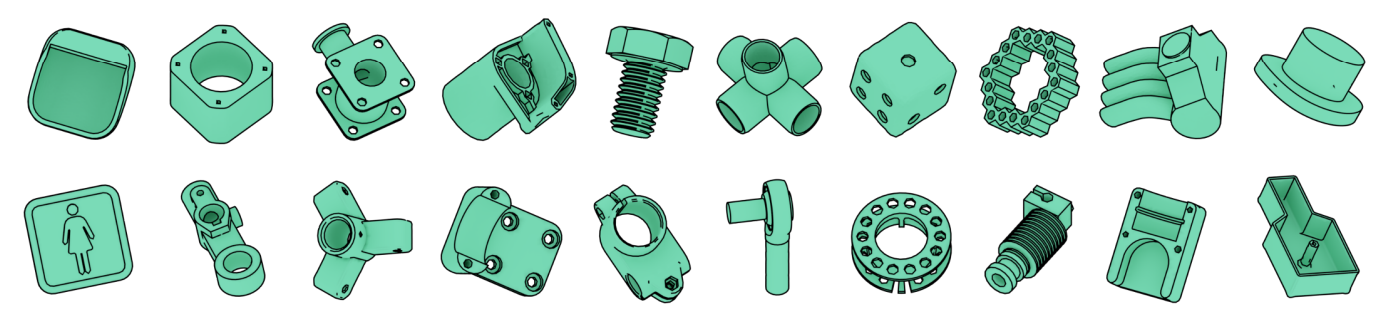
\includegraphics[width=350pt,height=150pt]{pictures/ABC.PNG}
    \caption{Some random objects from the ABC dataset.\cite{Koch_2019_CVPR}}
    \label{fig:abc}
  \end{figure}
\vspace{5mm}

The goal of this work is to develop a source library consisting of "good" source data which can be used as the data from the source domain in the further steps in a transfer learning pipeline. Therefore, the focus is to identify which features prevalent in an object makes it a "good" source data. A diverse collection of source data would be the objects that approximately captures the overall variance of the entire 1 million ABC dataset. Thus, it is trivial to think that more objects in the source library could better capture the overall variance of the dataset. But since the bin application is a model-based approach, it would be required to formulate the \ac{CAD} models of all these objects. Thus, having a large number of objects in the source library would entail high computational time for the generation of all the object models. Therefore, it is crucial to determine a permissible number of objects in the source library to facilitate its usage down the pipeline.  To further elaborate on this, if two objects are very similar to one-another than in spite of having a large similarity which just one other object, it loses the generalization capability of being nearly similar to a lot of other objects in the dataset. Hence, it would require a large amount of objects in the source library to capture the entire variance in the dataset. Thus, there is a trade-off between being very similar to a very small subset of objects and being approximately similar to a larger subset of objects in the dataset. Moreover, it is not universally defined which features in an object qualify as an important features and how it contributes in deciding whether an object is capable of becoming a viable source data. 
\subsection{Approach}
An end-to-end autoencoder proposed by \cite{mei2022unsupervised} is used to get the feature representations of the objects in the dataset\cite{Koch_2019_CVPR}. The autoencoder learns both the local and the global features of an object. Once the feature representation of the objects are obtained, they are grouped into clusters utilizing multiple clustering algorithm. A suitable clustering algorithm is utilized to get the representing members of the clusters. A high level overview of the entire method is shown in Fig. \ref{fig:overview}.
\begin{figure}[t]
  \centering
  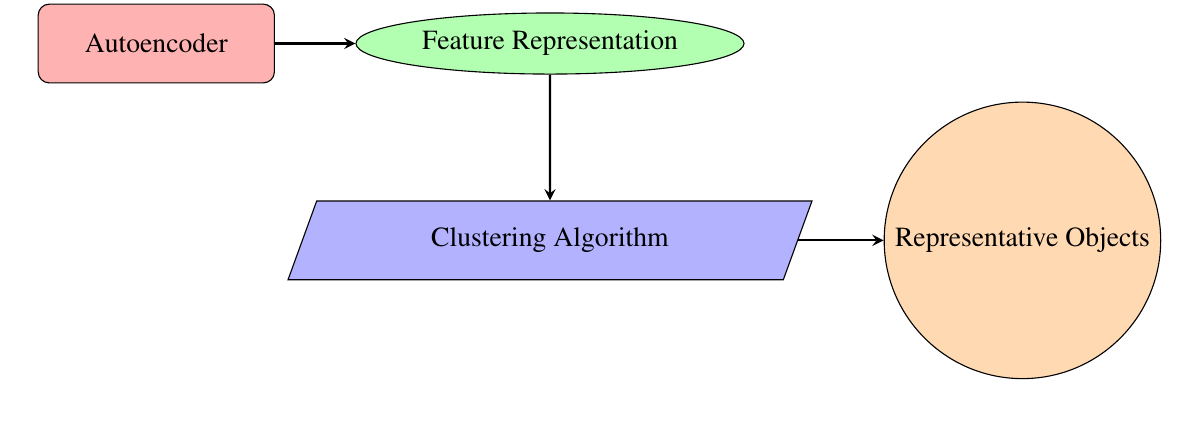
\begin{tikzpicture}[node distance=2cm]        
      \node (autoencoder) [Autoencoder] {Autoencoder};
      \node (feat_rep) [Feat_Rep, right of=autoencoder, xshift=3cm] {Feature Representation};
      \node (clustering_algorithm) [Clustering_algorithm, below of=feat_rep, yshift=-0.5cm] {Clustering Algorithm};
      \node (rep_objs) [Rep_Objs, right of=clustering_algorithm, xshift=4cm] {Representative Objects};
      \draw [arrow] (autoencoder) -- (feat_rep);
      \draw [arrow] (feat_rep) -- (clustering_algorithm);  
      \draw [arrow] (clustering_algorithm) -- (rep_objs);       
  \end{tikzpicture}
  \caption{Overview of the entire pipeline for development of source library.}
  \label{fig:overview}
\end{figure}
 The clustering algorithm would not just consider the Euclidean distance between the datapoints but also other intrinsic features of the dataset such as the density because real world datasets are not necessarily globular in structure. A suitable evaluation metric such as \ac{DBCV}\cite{moulavi2014density} is used to compare the quality of the clustering algorithms which is robust to the size and shape of individual clusters as well as the outliers and noise of the dataset. Since, computing the \ac{DBCV} index on the entire dataset is extremely computationally expensive, the evaluation is performed on random batches of the subset. Moreover, the \ac{DBCV} is sensitive to the number of features in the dataset and fails to provide any tangible result in the presence of a large number of features (e.g. over 150). Thus, a dimensionality reduction is necessary for the evaluation of the clustering algorithm. Once, the clustering algorithm with best results in the evaluation metrics is achieved the entire dataset is categorized into a number of clusters, where the medoid of the cluster is chosen as the representative member of the cluster. The similarity of the test dataset with the representative members of the datasets shows the generalization quality of the source library. The approximate time for each step of the work is shown in Tab. \ref{tab:overview_time}.

\begin{table}[ht]
  \caption{Overview of the approximate time taken for the creation of the source library}
  \label{tab:overview_time}
  \centering
  \begin{tabular}{|l|l|}
    \toprule
    Step & Time \\
    \midrule
    Training the model & 28 hours\\
    Dimensionality reduction & 4 hours \\        
    Clustering Algorithm & 3 hours \\
    Similarity evaluation & 11 minutes\\
    \bottomrule
  \end{tabular}
\end{table}
\subsection{Contribution}
Although density-based clustering algorithm like \ac{DBSCAN} and \ac{HDBSCAN} shows promising results when the clusters in real-world datasets aren't globular in nature, yet the current existing implementations in the literature doesn't put any restrictions on the number of clusters returned by the clusters. In case of very large datasets like the ABC dataset\cite{Koch_2019_CVPR}, these algorithms return a large number of clusters (over multiple thousands). The model generation of such thousands of objects aren't feasible or efficient in business situations such as in \ac{IPA}. Thus, novel contribution in this work is stated as follows:
\begin{itemize}
  \item The idea of multi-level \ac{HDBSCAN} algorithm is proposed in this work to limit the number of clusters to a feasible number but also retain the properties of a density based clustering algorithm.
  \item An extensive experimentation on the optimal hyperparameter values during model training has been carried on for the development of a high performing network used for the generation of feature representations of the objects in the dataset.
\end{itemize}
\cleardoublepage


\section{Related Work}
\label{sec:related_works}
This chapter provides a quick overview of the literature on unsupervised learning approaches for point clouds as well as variety of local feature extraction techniques on point clouds.

\vspace{5mm}


Since deep learning methods can directly process point clouds, feature learning for 3D objects has advanced significantly in the recent years. By independently learning every point in the point cloud and combining point characteristics with permutation invariant operations, PointNet \cite{qi2017pointnet} and Deep Sets \cite{zaheer2017deep} were the pioneers in the field to handle unordered and unstructured 3D points. Both \cite{qi2017pointnet} and \cite{zaheer2017deep} were important developments in deep learning for handling unordered data. \cite{qi2017pointnet} was designed particularly for 3D point cloud analysis, while \cite{zaheer2017deep} provides a broader framework for feature learning that is permutation invariant and could be extrapolated to graphs and sequences. These methods were capable to generate promising results. But it had limitations in learning the local features and hence needs further improvement to make them more scalable across different applications. PointNet++ \cite{qi2017pointnet++} enhances \cite{qi2017pointnet} by introducing a hierarchical feature learning technique that functions directly in a metric space. It has the ability to acquire knowledge at varying levels, the hierarchical arrangement of point clouds into nested partitions and combining sampling techniques that capture complex spatial relationships while maintaining permutation invariance. 


\vspace{5mm}

\cite{wang2019dynamic}  designed a \ac{DGCNN} architecture specifically for point cloud data. Its main contribution is to enable more efficient feature learning by dynamically building graph structures from point clouds based on local geometric correlations. But on the other hand, dynamic graph creation adds more computational complexity and might necessitate precise hyperparameter tuning. Although PointCNN \cite{li2018pointcnn} demonstrated state-of-the-art performance on a range of point cloud applications, the x-transformation adds to computational overhead and may restrict scalability, particularly when working with large-scale datasets.  But it provided a  permutation-invariant procedure that changes the orientation of point clouds to a canonical orientation enabling the use of standard convolutional operations. A deep learning architecture that directly operates on three-dimensional point clouds was introduced in \cite{wu2019deep}. 

\vspace{5mm}

The development of techniques for unsupervised representation learning on point clouds has been the focus of several works in the literature. These methods can be broadly classified as discriminative \cite{grill2020bootstrap} or generative \cite{sarmad2019rl}. The majority of techniques include autoencoding \cite{yang2018foldingnet} or \ac{GAN}s \cite{sarmad2019rl}.  Their primary method of operation is using an encoder to convert an input point cloud into a global latent representation \cite{rao2020global}, \cite{shi2020unsupervised}, or a latent distribution in the variational case \cite{hassani2019unsupervised}, \cite{han2019multi}, after which a decoder tries to reconstruct the input. High-level structural features can be effectively modeled by generative models. Nevertheless, a lot of these methods often work under the premise that every 3D item in a category has the same pose \cite{sanghi2020info3d}. Because of this assumption, these methods are sensitive to translation and rotation operations. Discriminative models, unlike generative methods, are trained to distinguish between data augmentations. It is seen that these methods produce good quality latent representations. Contrastive methods \cite{rao2020global}, \cite{sanghi2020info3d} have demonstrated impressive outcomes in recent unsupervised point cloud representation learning approaches, among discriminative models. Through data augmentation and comparison, contrastive approaches also enable the generation of rotation invariant representations \cite{poursaeed2020self}. Predicting a representation that is distant from the negative examples and closer to the positive ones is a crucial concept in contrastive learning \cite{chen2020simple}. But in order to perform better, these algorithms need a large number of negative examples to compare and rely largely on the selection of the negative samples and how they are paired alongside the positives \cite{grill2020bootstrap}, \cite{chen2021exploring}. Such an unsupervised method is typically computationally expensive and requires careful handling of the negative pairs, which can be achieved by relying on memory banks, huge batch sizes, or tailored mining strategies.\cite{grill2020bootstrap}

\vspace{5mm}

\cite{liu2019relation} presented a \ac{CNN} that incorporates relation-aware convolutional procedures which capture both local and global geometric relationships inside point clouds. Position-adaptive feature learning was the primary innovation of PAConv\cite{xu2021paconv}, which is the dynamic assembly of convolutional kernels based on local geometric structures. By using this method, the network performed better in segmentation and classification tasks by improving its capacity to detect intricate geometric patterns and variances within point clouds. The main contribution of AdaptConv \cite{zhou2021adaptive} was the inclusion of adaptive graph convolutional operations, which dynamically modify convolutional kernels receptive fields according to the point clouds local geometric characteristics. Because of the flexibility, the network can better execute tasks like segmentation and classification by capturing local and global geometric data. Convolutional operations adaptive nature might add more computational complexity. Moreover, the quality of local geometric information and intricacy of the point cloud may have a significant influence on the adaptive graph convolutional approach's efficacy, which may affect how well it performs in various datasets and applications. 

\vspace{5mm}

In \cite{sun2021quadratic}, a novel approach to encoding point clouds in three-dimensional (3D) space was presented. This method makes use of quadratic terms to more accurately describe local surface geometry. The capacity of the model to identify surface curvature and shape fluctuations is enhanced by the addition of quadratic components. As a result of including higher-order geometric information in the feature representations the discriminative ability of deep learning models were improved for point cloud segmentation and object classification tasks.  \cite{ding2021point} described how perturbation learning can improve the resolution of point cloud data. Its ability to generate high-resolution point clouds with improved geometric details is useful for 3D reconstruction and object detection applications. By using perturbation learning, the method can effectively capture fine-grained features and surface details, improving the overall quality of the unsampled point clouds. Also, the method can be applied to a variety of point cloud datasets because it is flexible and does not require any particular surface representations.  A new technique for geometric feature preservation in \ac{LiDAR} point cloud compression was reported by \cite{song2021layer}. This framework uses a layer-wise geometry aggregation approach to achieve lossless compression, which ensures that no information is lost across multiple layers of the point cloud.  The computational complexity of combining and evaluating geometric data across multiple levels could be a drawback. As more input point cloud data becomes available, this complexity might increase. \cite{zhao2021transformer3d} provided an innovative technique for improving the performance of 3D object detection by using transformer networks to refine votes. It combines and refines votes from different parts of the point cloud to enhance object recognition. This method increased accuracy and robustness in 3D object identification tasks. While these approaches were remarkably successful, in order to do feature learning, they need supervised data. Point cloud models are difficult to implement in novel real-world scenarios where labelled data is hard to come by due to their reliance on annotation. Therefore, its critical to devise strategies for lowering the quality of annotated samples needed to complete deep learning-based point cloud interpretation tasks with the necessary performance\cite{mei2022unsupervised}.
\cleardoublepage

\section{Fundamentals}
\subsection{Bin Picking}
\subsubsection{Definition and Application}
Bin picking is a robotics and automation technique used in manufacturing and logistics, automotive industry, particularly in warehouses and assembly lines. It involves locating, grabbing and manipulating objects from a bin or container utilizing robotic devices equipped with sensors, cameras and algorithms. Thus, it is a crucial area of interest for research in computer vision and robotics. There are usually multiple steps in the process: sensing and perception, planning and path calculation, grasping and manipulation, ultimately transportation and placement which will be further elaborated in the following passages.\cite{bin_picking}

\vspace{5mm}

\textbf{Sensing and Perception} To determine the kind position orientation and the kind of objects inside a bin or container, the robot uses its sensors and cameras to scan it. For the purpose of identifying the items, especially ones that are partially occluded or organized randomly or have entanglement in between them, advanced computer vision algorithms are used for the purpose.\cite{bin_picking}

\vspace{5mm}

\textbf{Planning and Path Calculation} Following the identification of the items in the bin, the robots control system determines the best course for the arm or gripper to take in order to reach and retrieve the intended item in the bin. Avoiding collision with other objects in the bin and calculating the most efficient path for carrying the objects from one point to another are the two crucial parts in this stage. \cite{bin_picking}
\vspace{5mm}

\textbf{Grasping and Manipulation} The robot can places its arm in a suitable location and employs its gripper to firmly hold the object of interest. Firm and control over the grippers is crucial for this stage to prevent damage and unwanted slippage.\cite{bin_picking}

\vspace{5mm}

\textbf{Transportation and Placement} Once the robot has a firm grip on the object it moves the item to the intended spot, like a shipping container, assembly line or conveyor belt. Before settings the object down, the robot occasionally needs to realign or orient it.\cite{bin_picking}

There are numerous benefits of bin picking in manufacturing and logistics.
\begin{itemize}
  \item \textbf{Enhanced Efficiency} Businesses can greatly boost productivity and throughput, particularly in high-volume operations, by automating the process of selecting goods from bins.
  \item \textbf{Flexibility} Bin picking applications are appropriate for a variety of manufacturing situations because they can handle a wide range of items based on their shapes, size and materials.
  \item \textbf{Savings} Automating manual labor-intensive jobs, such as bin picking, can save labor costs and lower the chance of accidents that come with physical handling.
  \item \textbf{Health of Employees} Picking heavy objects for a longer period of time can often be detrimental for the worker's health. Thus, using automated bin picking solutions can be extremely helpful in such cases.
\end{itemize}
Keeping everything in mind, bin picking applications are essential to contemporary manufacturing and logistic operations, helping businesses to increase productivity and streamline workflows.
\subsubsection{Gripper Types}
Grippers are crucial parts of robotic systems used in bin picking applications that allow them to grab and move objects out of the bins or containers. There are different kinds of grippers and each is appropriate for a particular purpose depending on the shape, size, weight and substance of the objects being handled. The following are a few typical gripper kinds used for bin picking.

\vspace{5mm}

\textbf{Vacuum Grippers} These grippers cling to smooth or flat  surfaces using suction as shown in Fig. \ref{fig:vacuum_gripper}.
\begin{figure}
  \centering
  \begin{minipage}[t]{.45\textwidth}
    \centering
    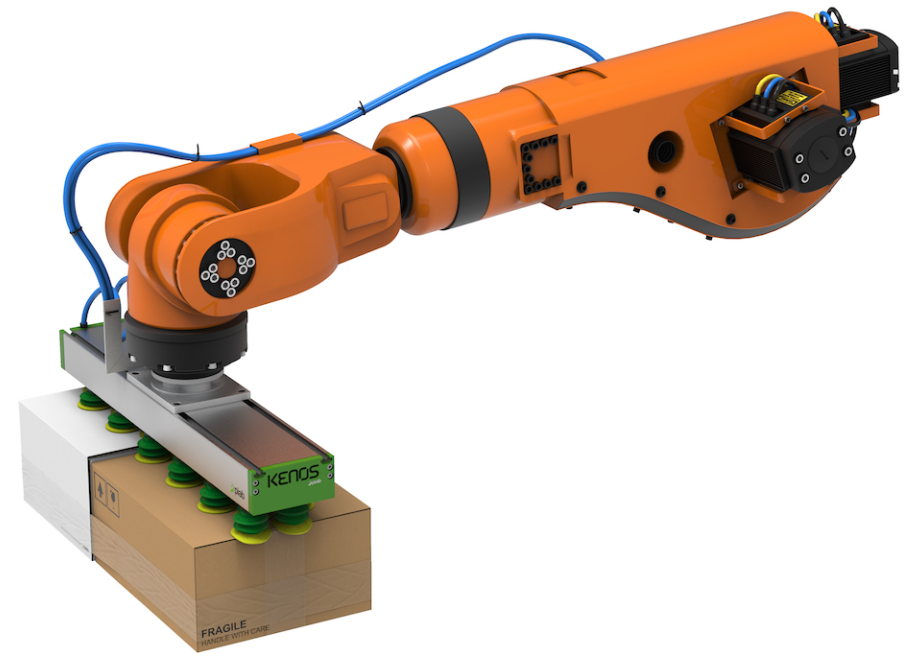
\includegraphics[width=150pt,height=150pt]{pictures/vacuum_gripper.png}
    \captionof{figure}{Vacuum Grippers\cite{vacuum_gripper}}
    \label{fig:vacuum_gripper}
  \end{minipage}%
  \hspace{1cm}
  \begin{minipage}[t]{.45\textwidth}
    \centering
    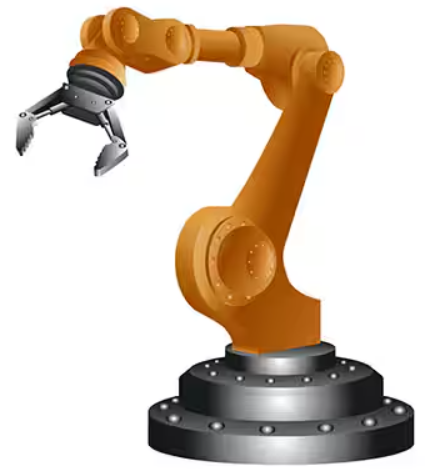
\includegraphics[width=150pt,height=150pt]{pictures/mechanical_gripper.png}
    \captionof{figure}{Mechanical Grippers\cite{mechanical_gripper}}
    \label{fig:mechanical_gripper}
  \end{minipage}
\end{figure}
When handling huge, flat good like sheets of plastic, glass or metal, they are especially useful. By using interchangeable suction cups or pads, vacuum grippers can be made to handle objects of various sizes and shapes. The primary advantage of these type of grippers is the need for one-surface accessibility. This makes handling cluttered bins easier. The drawback however is that a vacuum gripper can still generate traction even if the intended grasping position is not met. This results in a possibly erroneous placement and an imprecise position of the gripper.\cite{spenrath2022heuristic}

\vspace{5mm}

\textbf{Mechanical Grippers} To grasp objects, mechanical grippers use mechanical jaws, fingers or claws. They may be tailored with various jaw configurations to meet particular object geometries and are appropriate for a broad variety of shapes and sizes. Mechanical grippers are useful for picking up objects with uneven shapes, such as bottles, crates and components, as they offer a solid hold as shown in Fig. \ref{fig:mechanical_gripper}. But because of the tough and rigid mechanical nature of the gripper, it might cause damage while handling delicate and sensitive objects.\cite{fager2020gripper}

\vspace{5mm}

\textbf{Magnetic Grippers} These devices draw in and hold onto ferromagnetic materials like steel using electromagnetic forces as shown in Fig. \ref{fig:magnetic_gripper}.
\begin{figure}
  \centering
  \begin{minipage}[t]{.45\textwidth}
    \centering
    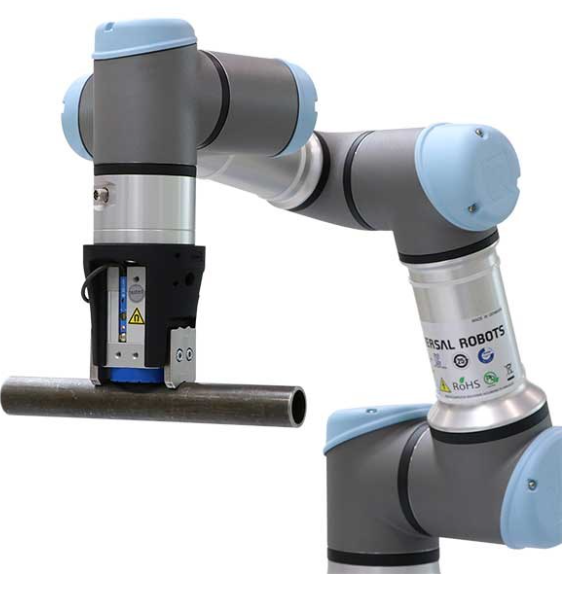
\includegraphics[width=150pt,height=150pt]{pictures/magnetic_gripper.PNG}
    \captionof{figure}{Magnetic Grippers\cite{magnetic_gripper}}
    \label{fig:magnetic_gripper}
  \end{minipage}%
  \hspace{1cm}
  \begin{minipage}[t]{.45\textwidth}
    \centering
    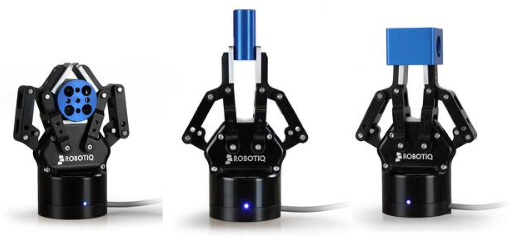
\includegraphics[width=200pt,height=100pt]{pictures/adaptive_gripper.PNG}
    \captionof{figure}{Adaptive Grippers\cite{adaptive_gripper}}
    \label{fig:adaptive_gripper}
  \end{minipage}
\end{figure}
As such, the benefits and drawbacks are similar to those of vacuum grippers. They are appropriate for applications where cleanliness or delicate surfaces are a concern since they are perfect for handling metallic objects without the need for direct contact. Because of its magnetic properties, it can induce magnetic behavior to the objects being handled which is not desirable and can have serious implication in certain applications\cite{spenrath2022heuristic}. Furthermore, it is possible that the gripper might grab multiple objects at a time instead of a single object which is not desirable.\cite{spenrath2022heuristic} 

\vspace{5mm}

\textbf{Adaptive Grippers} These grippers can handle a broad range of sizes and forms without the need for exact placement since they are made to conform to the shape of the object being held as shown in Fig. \ref{fig:adaptive_gripper}. These grippers frequently modify their shape to fit the curves of the object by using inflated bladders or flexible  polymers. However, to facilitate its adaptive property, it demands for complex control algorithms for precise grasping.\cite{park2018hybrid}

\vspace{5mm}

\textbf{Soft Grippers} Designed to softly grab delicate or unusually shaped objects without causing damage, soft grippers are created from responsive materials like silicone or rubber as shown in Fig. \ref{fig:soft_gripper}. 
\begin{figure}
  \centering
  \begin{minipage}[t]{.45\textwidth}
    \centering
    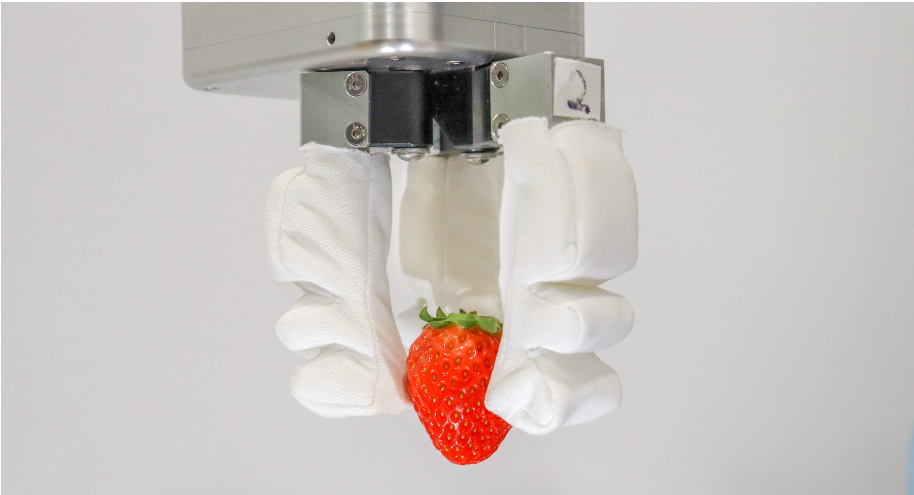
\includegraphics[width=170pt,height=120pt]{pictures/soft_gripper.PNG}
    \captionof{figure}{Soft Grippers\cite{soft_gripper}}
    \label{fig:soft_gripper}
  \end{minipage}%
  \hspace{1cm}
  \begin{minipage}[t]{.45\textwidth}
    \centering
    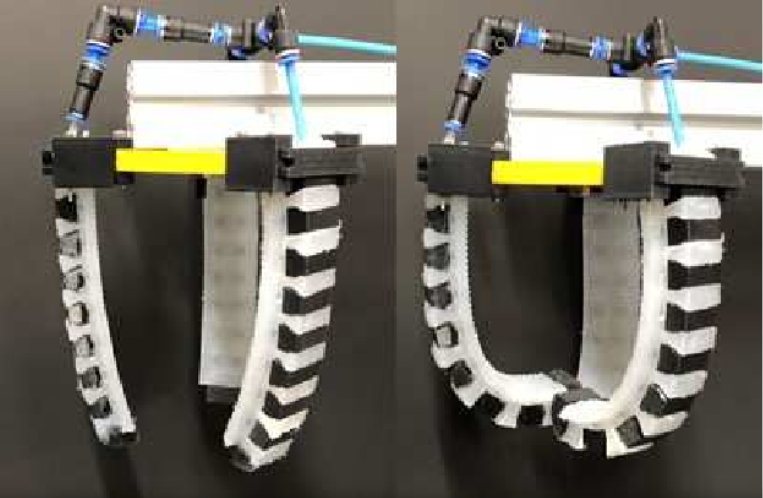
\includegraphics[width=170pt,height=120pt]{pictures/hybrid_grippers.PNG}
    \captionof{figure}{Hybrid Grippers with soft and rigid structures\cite{park2018hybrid}}
    \label{fig:hybrid_gripper}
  \end{minipage}
\end{figure}
They are frequently employed in tasks like picking up food or electrical components, where dexterity and delicate handling are crucial. However, they have lower gripping force as compared rigid grippers, thus, limiting suitability for heavier objects.\cite{park2018hybrid} 

\vspace{5mm}

\textbf{Hybrid Grippers} To improve performance and versatility, hybrid grippers integrate many grasping techniques such as vacuum suctions and mechanical clamping. These grippers are frequently employed in intricate bin picking scenarios where a solitary gripping technique would not be adequate. It also requires more calibration and maintenance due to the integration of multiple systems. It also leads to greater power consumption and computational overhead for executing hybrid gripping mechanism. Thus, the characteristics of the objects being handled, the capabilities of the robotic system and the particular requirements of the application all play a role in the gripper selection. Stakeholders can maximize the effectiveness, dependability and precision of their bin picking processes by choosing the right kind of gripper.\cite{park2018hybrid} 

\subsubsection{Model-Based Approaches}
Model-based  bin picking approaches use a digital model or representation, of the items in the bin as a guide for organizing and carrying out the bin picking procedure. To enable accurate perception and manipulation, these methods make use of \ac{CAD} data or 3-D models of the items. Fig. \ref{fig:model_based} 
\begin{figure}[t]
  \centering
  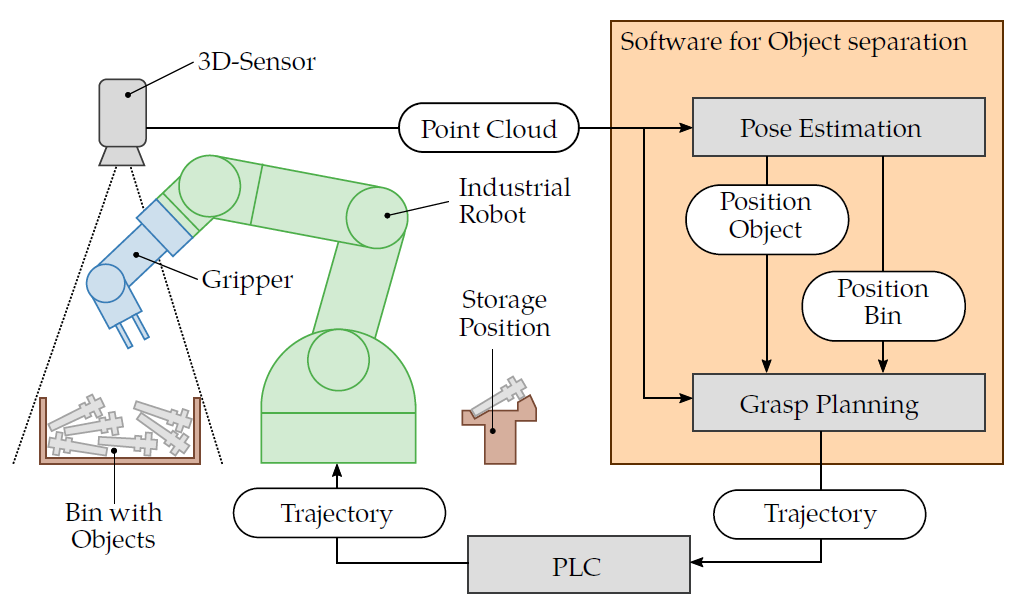
\includegraphics[width=400pt,height=250pt]{pictures/model_based.PNG}
  \caption{Overview of model-based bin picking approach.\cite{spenrath2022heuristic}}
  \label{fig:model_based}
\end{figure}
gives an overview of model-based bin picking approach, an elaboration of which is provided below.

\vspace{5mm}

\textbf{Object Modelling} Creating precise digital models of the objects to be picked is the first stage in a model-based bin-picking strategy. \ac{CAD} software or 3D point cloud generated from real objects through scanning methods like laser scanning or photogrammetry can be used for this. The model ought to be accurately represent the objects surface features, size and geometry.\cite{lin2020robotic}

\vspace{5mm}

\textbf{Bin Perception} The robots sensors, including depth cameras or laser scanners, record information about the contents of the bin once the object models are accessible. Based on the shape, size and orientation of each object in the bin, this data is processed to identify and segment each of them. In order to match and align the perceived objects with their corresponding models, the digital models are used as reference templates.\cite{lin2020robotic}

\vspace{5mm}

\textbf{Pose Estimation} It is the process of figuring out each recognized object's exact location and orientation with respect to the gripper or end effector of the robot. Planning precise gripping trajectories and guaranteeing successful object manipulation depend on this phase. Pose estimation methods include geometric fitting algorithms, point cloud registration and feature mapping.\cite{lin2020robotic}

\vspace{5mm}

\textbf{Grasping Planning} Once the posture of the object is determined, the robot arranges its arm to grasp the object from the bin. In order for the robot's arm or gripper to approach, grasp and safely lift each object, collision-free motion path needs to be calculated. To enable successful gripping, planning algorithms take into account variables including gripper kinematics, object geometry and workspace limitations.\cite{lin2020robotic}

\vspace{5mm}

\textbf{Feedback Control} To monitor and modify the robot's movements in real-time while it is grasping, feedbacks from the sensors such as force/torque sensors or vision systems is utilized. By using feedback control approaches, the robot may adjust its grip in response to unforeseen disruptions or changes in the surroundings, guaranteeing dependable and durable picking performance.\cite{lin2020robotic}

\vspace{5mm}

\textbf{Validation and Verification} The system compares the actual results with the predicted result based on model-based planning to determine whether the grasp was successful after selecting each object. Verifying grasp stability, item alignment and adherence to quality standards are a few examples of validation tasks. The robot can rectify any mistakes by trying to pick the object again or modifying its approach.\cite{lin2020robotic}

\subsubsection{Model-Free Approaches}
The goal of model-free bin picking approach is to pick objects from a bin without using \ac{CAD} data or predefined object models. To identify and handle objects based solely on sensor data, these methods use advanced machine learning algorithms and complex perception techniques. Model-free approaches can be broadly categorized into two groups: deep-learning based approach\cite{bousmalis2018using}, reinforcement learning based approach\cite{levine2018learning} and hybrid perception-based approach\cite{jang2018grasp2vec}. 

\vspace{5mm}

\textbf{Deep Learning-Based Approach} Without explicitly modelling the objects, deep learning techniques like \ac{CNN}s are trained on massive amount of sensor data to learn object recognition and grasping policies on their own. Labelled object instances and corresponding grasping actions are collected from large datasets of sensor data (e.g. \ac{RGB} images, depth maps). Using end-to-end optimization, \ac{CNN}s are trained on those data to acquire grasping policies and object representations. Based on sensor input, robotic systems with trained models are able to grasp objects and identify them in real-time. To enhance grip execution and boost performance, feedback from sensors (such as force/torque sensors) are employed.\cite{bousmalis2018using}

\vspace{5mm}

\textbf{Reinforcement Learning-Based Approach} Without explicit object models, robots can acquire grasping policies through trial and error interactions with the environment by using \ac{RL} techniques. By performing grasping movements and getting feedback (like reward signals) when a task is completed successfully, the robot interacts with its surroundings(e.g. a bin). \ac{RL} algorithms learn grasping policies by optimizing the total rewards earned from the accomplished grasps and interactions with the surroundings. In order to maximize the performance, \ac{RL} agents strike a balance between exploring novel grasping tactics and utilizing previously learnt rules. Robotic systems are equipped with capability to perform bin-picking tasks in real-time.\cite{levine2018learning}

\vspace{5mm}

\textbf{Hybrid Perception-Based Approach} Robots can learn grasping rules from data by combining perception and action primitives in hybrid techniques, which also incorporate domain knowledge or limitations. Using deep learning models or conventional computer vision approaches, sensor data (e.g. \ac{RGB} images) is processed to extract object representation or features. A combination of  imitation learning and reinforcement learning is used to learn grasping policies. Using the learnt policies and the sensor data, perception and action modules work together to optimize the grasping performance. The learnt policies are improved over time by adjusting the grip execution based real-time data from sensors.\cite{jang2018grasp2vec} 

\subsubsection{Robot System}
For pick and place tasks, delta robots and parallel kinematics are the usual system. For bin-picking applications, however, serial kinematics and articulated robots are the more popular options. The advantages include, a much bigger workspace, more degrees of freedom for the end-effector or gripper, allowing a wider range of gripping poses and less limitations sue to internal collisions. The robot system's main task is to match various positions. The following are the three crucial ones for bin picking systems.\cite{spenrath2022heuristic}
\begin{itemize}
  \item The position of the object $\mathbf{W_{P_O}}$ characterizes the object's position in relation to the world coordinates.
  \item The position of the gripper $\mathbf{W_{P_G}}$ characterizes the end-effector's position in relation to the world coordinates.
  \item The grasping position $\mathbf{G_{P_O}}$ characterizes the position of the object in relation to the position of the gripper. This is particularly crucial foe the object's precise placement. 
\end{itemize}
These three positions constitute the closed transformation chain. In other words, the computation of the third pose is easy if the first two are known. These three poses are shown in Fig. \ref{fig:robot_workspace}
\begin{figure}[t]
  \centering
  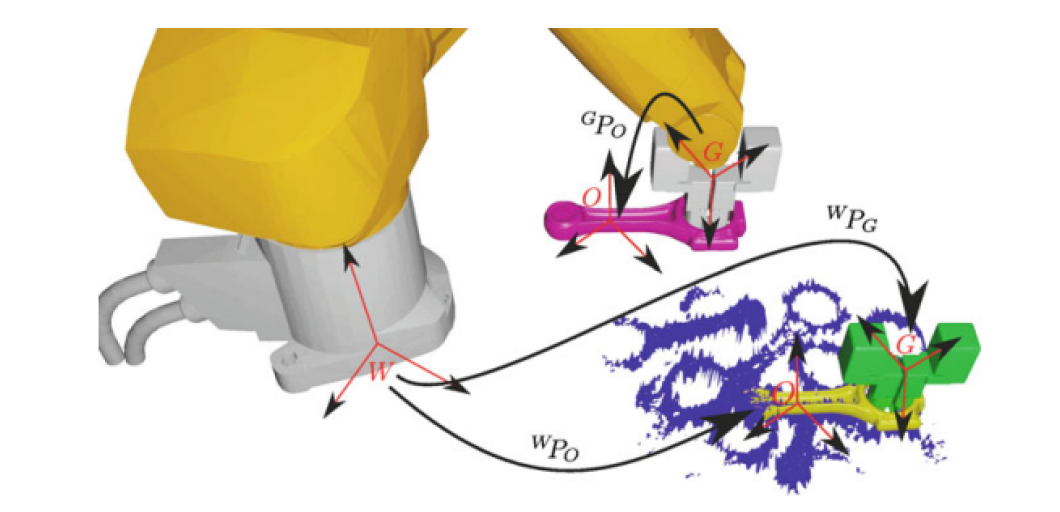
\includegraphics[width=400pt,height=250pt]{pictures/robot_pose.PNG}
  \caption{Important positions of the workspace in a  bin-picking application. $W$ is the world coordinate system with its origin at the centre of the base of the robot. $O$ is the object coordinate system with its origin at the center of the object. $G$ is the gripper coordinate system with its origin at the center of the gripper.\cite{buchholz2015bin}}
  \label{fig:robot_workspace}
\end{figure}
A robot can place its end-effector using one of the two movement techniques: \ac{LIN} motion and \ac{PTP} motion. Every robot motor moves synchronously when in \ac{PTP} motion. Generally speaking, figuring out the trajectory of the \ac{TCP} is difficult when in this mode. The benefit of this motion, however, is its potential to achieve maximum speed. Because of this, this mode is employed to travel great distances between certain poses. The \ac{TCP} is a crucial point in the \ac{LIN} motion. In this motion, the \ac{TCP} travels linearly from one place to another in Cartesian space. Its speed is much slower than in \ac{PTP}, which is a drawback for confined workspaces. Inverse kinematics calculation and singularity avoidance are the two components of the \ac{LIN} mode operation. These configurations are typically detected by robot controller, which will stop the robot.\cite{spenrath2022heuristic}

\subsection{Deep learning-based 3D Image processing}
\subsubsection{Convolution Neural Network}
Inspired from the visual cortex of humans, (\ac{CNN} or ConvNet) is a type of deep neural network designed for processing data which appear in a grid like manner like images, videos, etc.  It was introduced by LeCun et. al in \cite{lecun1998gradient} in 1998.  It gets its name because of the usage of a special kind of linear mathematical operation called the convolution instead of using matrix multiplication as prevalent in the pre-existing neural networks. The key components of a \ac{CNN} are - Convolution layer, activation function, pooling layer, loss function, output layer. The principle building block of a CNN is the convolution layer. It consists of a number of learnable filters (kernels) which can be visualized like a cubic block. The success of \ac{CNN}s can be attributed to three major concepts: sparse interactions, parameter sharing and equivariant representations.\cite{Goodfellow-et-al-2016}
\paragraph{Sparse interactions}
In traditional fully connected network, matrix multiplication is performed which involves a parameter matrix. The interaction between input and output units are captured by a distinct parameter in the parameter matrix. But \ac{CNN}s have sparse interactions, i.e. only a subset of units or neurons in a layer is connected to a local region in the preceding layer. This is done by using kernels that are significantly smaller than the input. This implies, less number of parameters need to be stored which reduces the memory consumption and also it is computationally efficient because it has to perform fewer operations. For example, if there are $m$ inputs and $n$ outputs, the fully connected network would need to store \textit{m} x \textit{n} parameters and have a runtime of \textit{O}(\textit{m} x \textit{n}) time complexity per input. On the other hand, if the number of connections for each unit is restricted to be $k$, then there would be \textit{k} x \textit{n} parameters and have a runtime of \textit{O}(\textit{k} x \textit{n}) time complexity per input, where $k$ is quite some fold lesser in magnitude as compared to $m$. Moreover, since convolution layers are stacked upon one another in a deep convolution network, units in the deeper layers have a larger receptive field, because of its indirect interaction with a larger region in the input.
\paragraph{Parameter sharing}
Another important focus behind using the convolution layer was to reduce the number of parameters in a \ac{FCN}. For example in a 1024*1024 image, a \ac{FCN} would have over 1 million hidden units, which means it would have over 1 trillion trainable parameters. But the pixels in an image are only locally correlated. So, \ac{CNN}s make use of the kernels to limit the focus on smaller regions on the image at a time known as the receptive field. This significantly reduces the number of trainable parameters, thus, reducing the memory consumption \cite{ConvNet}. These layers perform a convolution operation between the input (eg. image) \textit{I} and the kernel \textit{K} to produce an output \textit{S} known as the feature map as in Eq. \ref{eq:conv}.\cite{Goodfellow-et-al-2016}
\paragraph{Equivariant Representations} 
A function is said to be equivariant if the input to a function is changed, then the output changes in the similar way. Because of the parameter sharing mechanism, convolutions operations are translation equivariant. When the kernels are applied on an input image, the convolution layers generate a 2D map of where the particular feature occurs in the particular image. Furthermore, a pixel is related to its neighboring pixels to form a meaningful context(create a feature e.g. an edge in an image) but it is not limited to where it can occur throughout the image. Thus, it creates multiple filters each of which look for the same feature throughout the image. But it is also to be kept in mind that convolution is not equivariant to other geometric and affine transformations like rotation, scaling, etc. 
 Since convolution operations are commutative in nature, Eq. \ref{eq:conv} can also be written as Eq. \ref{eq:conv_com}. Typically, Eq. \ref{eq:conv_com} is easier to incorporate into a machine learning library since values for both $'m'$ and $'n'$ varies within a small range.\cite{Goodfellow-et-al-2016}
\begin{equation}
    \label{eq:conv}
    \mathit{S(i,j)}= \mathit{(I*K)(i,j)} = \sum_{m}\sum_{n}\mathit{I(m,n)K(i-m,j-n)}.
\end{equation}
\begin{equation}
    \label{eq:conv_com}
    \mathit{S(i,j)}= \mathit{(I*K)(i,j)} = \sum_{m}\sum_{n}\mathit{I(i-m,j-n)K(m,n)}.
\end{equation}
\paragraph{Activation function}
The next step in a \ac{CNN} is to apply an activation function. the purpose of using a non linear activation function is to capture the non-linearity in the data. Moreover if non-linearity is not used in between the multiple layers of a neural network, the network is effectively only one layer deep which is not capable even to capture the non-linearity in real world datasets. \ac{ReLU} is the most commonly used non-linear activation function used in \ac{CNN}s because unlike sigmoid function or tanh function it does not penalise "too correct" data points. Another remarkable benefit of using \ac{ReLU} is its ability to propagate gradient through deep networks with a constant factor. Also it is more memory efficient to use \ac{ReLU} as it doesn't require to store the \ac{ReLU} outputs separately as compared to tanh outputs.\cite{Goodfellow-et-al-2016}
\paragraph{Pooling}

\begin{figure}[t]
  \centering
  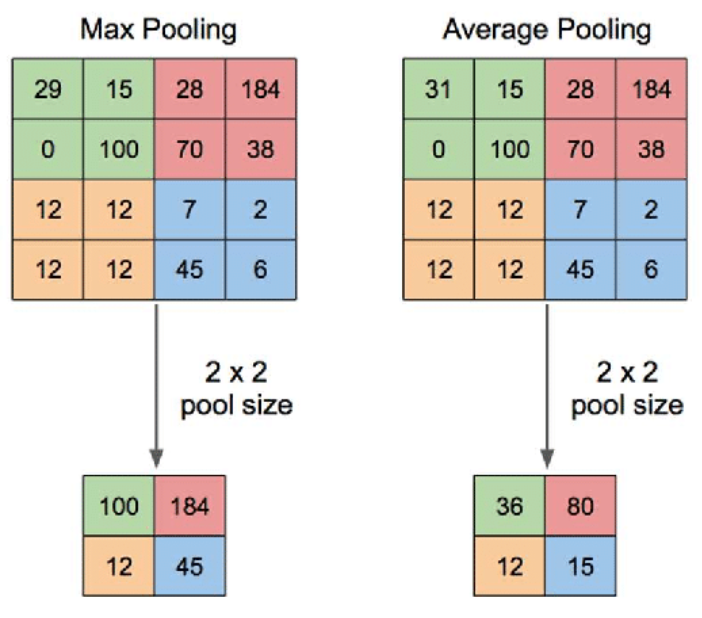
\includegraphics[width=400pt,height=250pt]{pictures/pooling.PNG}
  \caption{Max pooling operation on the left and average pooling operation on the right.\cite{pooling}}
  \label{fig:pooling}
\end{figure} 

The third step of a \ac{CNN} is to use the pooling layer. The main purpose of this operation is to make the detection of the features robust to the exact location of the eye (i.e. invariant to small translations). The different types of pooling operations are - max pooling and average pooling. It also helps in reducing the dimensionality of the input without losing too much information. This is done to make the computations faster down the deeper layers of the network. If the pooling operations are performed after every k pixels, then the next layer processes inputs that are k times lesser as shown in Fig. \ref{fig:pooling}. As the name suggest, the maximum value within the kernel is taken during max-pooling and the average value during average pooling. Since the number of parameters in a layer are dependent on the size of the input to the layer, it significantly reduces the computational overhead on using pooling operations.

\paragraph{Batch Normalization}
Another very important aspect in \ac{CNN} is batch normalization. In this step, it takes the output of the convolution layer and reassigns the pictures in the feature maps to a new mean and standard deviation. At first, the pixels values are normalized by calculating the z-score of all the pixels. It is then multiplied by a learnable parameter commonly referred as alpha which denotes the range and is then added to another learnable parameter beta which controls the offset value as shown in Eq. \ref{eq:batch_norm}. 
\begin{equation}
  \label{eq:batch_norm}
  x'= (\frac{(x-mean)}{standard \, deviation} \times alpha) + beta,
\end{equation}
where $x'$ is the normalized value after each batch, $x$ is the value of the pixel in the feature map. Batch normalization method is crucial because it handles the exploring gradient problem. 

\subsubsection{Autoencoders}
\begin{figure}
  \centering
  \begin{minipage}[t]{.45\textwidth}
    \centering
    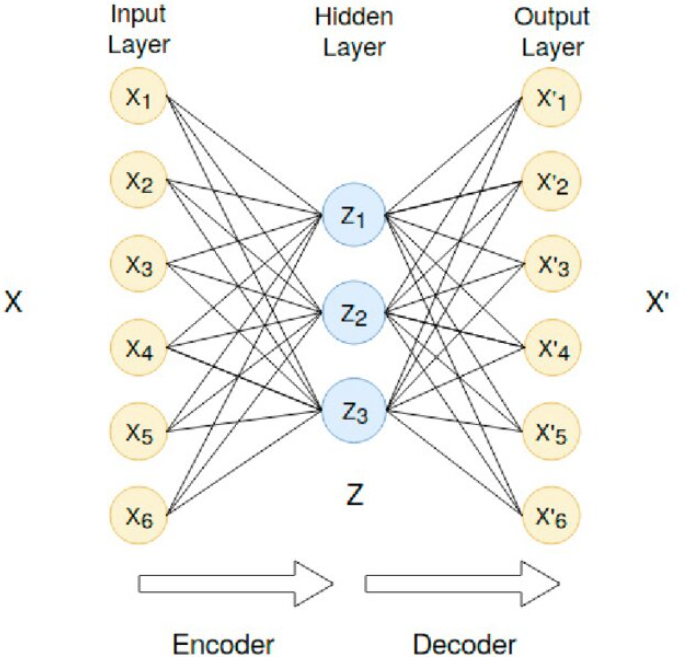
\includegraphics[width=200pt,height=150pt]{pictures/undercomplete_autoencoder.png}
    \captionof{figure}{Architecture of an undercomplete autoencoder.\cite{undercompleteautoencoder}}
    \label{fig:undercompleteautoencoder}
  \end{minipage}%
  \hspace{1cm}
  \begin{minipage}[t]{.45\textwidth}
    \centering
    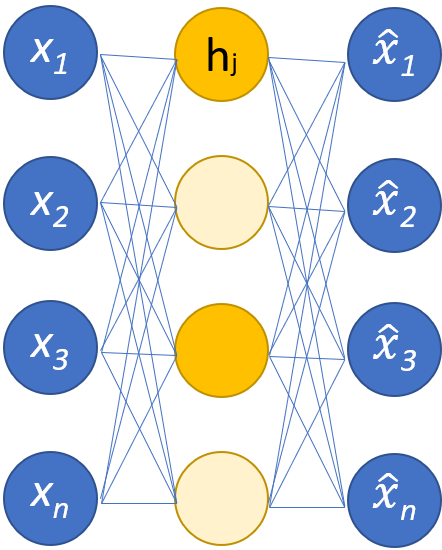
\includegraphics[width=200pt,height=150pt]{pictures/sparse_autoencoder.png}
    \captionof{figure}{Architecture of a single layer sparse encoder. The hidden nodes in bright yellow are active, while the ones in light yellow are set to zero, hence inactive\cite{autoencoder}}
    \label{fig:sparse_autoencoder}
  \end{minipage}
\end{figure}
Autoencoders are a special type of feedforward neural network in which the output tries to reconstruct the input. It is predominantly used in unsupervised learning for the tasks if dimensionality reduction, learning feature representations and for data compression. It tries the encode the input data into a more compact representation with lower dimensions called the "code"\cite{Goodfellow-et-al-2016} or "latent space". The idea is that this latent space representation should capture the most vital aspects of the input data. This is done by the first part of the network called the encoder. The second part of the network, the decoder then tries to decode this compressed representation of the input data to reconstruct the original input data as accurately as possible. During the training of an autoencoder, the goal is to minimize this reconstruction loss, i.e. the difference between the original input data and the output of the decoder. There are different types of autoencoders - undercomplete autoencoders, convolutional autoencoders, regularized autoencoders and variational autoencoders.

\vspace{5mm}


Undercomplete autoencoders ensure that the dimension of the latent space representation is less than the dimension of the original input data as show in Fig.\ref{fig:undercompleteautoencoder}. The output of the decoder to be the exact copy of the input is of no use. Rather, if the dimension of the code is less than that of the input, then it ensures that the autoencoder learns those representative features of the input data which are most salient\cite{Goodfellow-et-al-2016}. Convolutional autoencoders are an extension of traditional autoencoders where convolution layers are used as building blocks in both the encoder and the decoder part of the autoencoder. After training the network, the encoder part is used for extracting the features of the data and the decoder part is used for the reconstruction of the input data.

\vspace{5mm}

\begin{figure}[t]
  \centering
  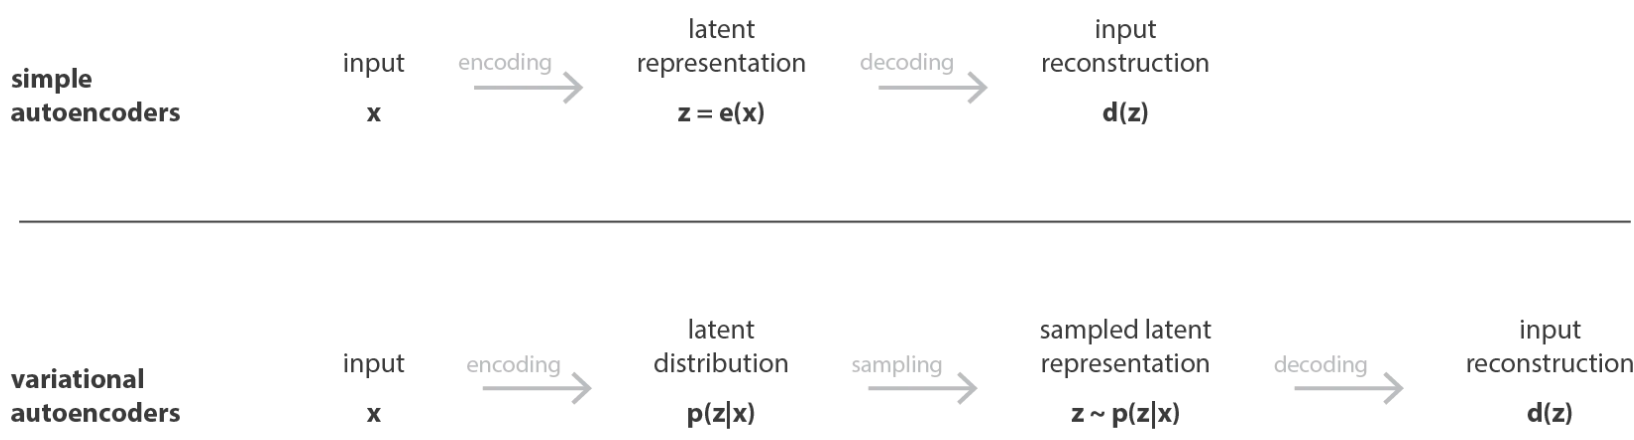
\includegraphics[width=400pt,height=150pt]{pictures/vae.png}
  \caption{Difference between a vanilla autoencoder and a \ac{VAE}.\cite{vae_image}}
  \label{fig:vae}
\end{figure} 
Regularized autoencoders are a special type of autoencoders that employs one or more regularization techniques to prevent the model from overfitting. The different types of regularizations used are L1 or L2 Regularization which add a penalty to the loss function depending on L1 or L2 norm of the model weights. As a result of this, the model is capable of learning sparse representation of the training data where many weights are set to a very small value or zero as shown in Fig\ref{fig:sparse_autoencoder}. Dropout is also used as a regularization technique where a percentage of the model's nodes are set to zero during training so that the model doesn't rely heavily on the weight of any particular node, thus, preventing overfitting and improving generalization on unseen data. 

\vspace{5mm}

The previously mentioned regularization techniques give rise to a variation of regularized autoencoders called the sparse autoencoders\cite{ng2011sparse}. Sometimes noise is also added to the training data or the hidden layers of the model to increase the robustness the model giving rise to denoizing autoencoders\cite{vincent2008extracting}. One more regularization technique is to apply a contractive regularization term based on Frobenius norm of the Jacobian matrix of the model's hidden layer activations with respect to the input data\cite{rifai2011contractive,autoencoder}. This ensures that a small neighborhood of the input data corresponds to a small neighborhood in the latent space representation, which means small perturbations in the input data leads to small or zero variation in the latent space representation\cite{rifai2011contractive,autoencoder}. By doing so, it makes the model more robust to small changes in the input data, thus, preventing overfitting.

\vspace{5mm}

\ac{VAE}s are a distinct type of autoencoders which produces latent space representations that are continuous. This allows random sampling and interpolation for the generation of new datapoints. The difference between a vanilla autoencoder and a \ac*{VAE} is shown in Fig.\ref{fig:vae}. Instead of producing a single vector for the latent space representation, it generates two vectors: a vector of means $\mu$ and a vector of standard deviations $\gamma$ for all datapoints. An encoding is then sampled from a distribution with mean $\mu$ and standard deviation $\gamma$. Thus, even for the same input, i.e. when the mean and the standard deviation are the same, the sampled encoding would vary because of the involvement of the sampling procedure. The mean vector controls the position where the encoding of the input should have its centre and the standard deviation controls the area over which the sampled encoding is allowed to vary from the mean. As a result of this, the decoder learns to decode not just the encoding of a single point but also the points in the neighborhood and hence a continuous latent space representation is obtained. In order to ensure that the latent space representation satisfies that the nearby encoding are similar to each other on a local scale while also facilitating interpolation on a global scale \ac{VAE}s jointly optimizes the reconstruction loss and the \ac*{KL}\cite{kullback1951information} loss.\cite{kingma2019introduction,vae}

\subsubsection{Siamese Network}
\begin{figure}
  \centering
  \begin{minipage}[t]{.45\textwidth}
    \centering
    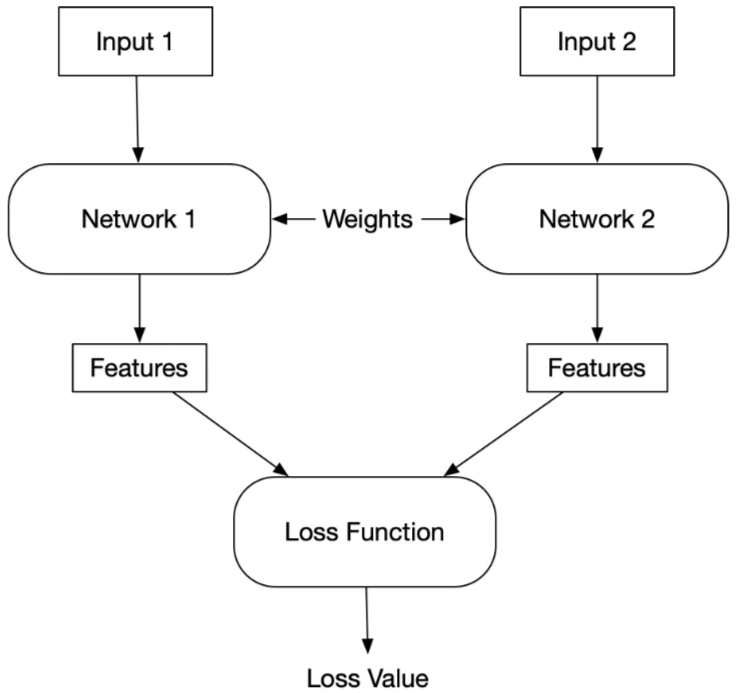
\includegraphics[width=200pt,height=120pt]{pictures/siamese_network.png}
    \captionof{figure}{A generic Siamese Network.\cite{siamese_network}}
    \label{fig:siamese_network}
  \end{minipage}%
  \hspace{1cm}
  \begin{minipage}[t]{.45\textwidth}
    \centering
    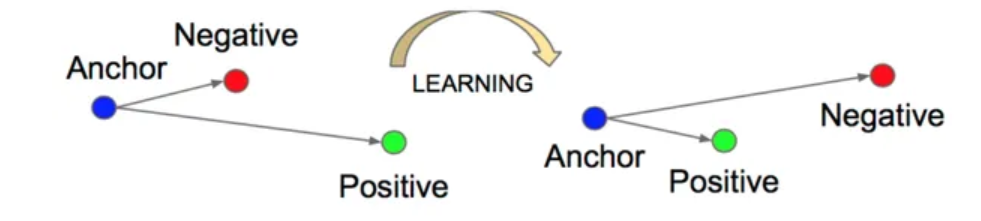
\includegraphics[width=200pt,height=100pt]{pictures/triplet_loss.PNG}
    \captionof{figure}{Before (left) and after (right) minimizing triplet loss function\cite{triplet_loss}}
    \label{fig:triplet_loss}
  \end{minipage}
\end{figure}
Traditional deep learning models have shown ground breaking results in a multitude of applications like image recognition and classification, web scraping, speech recognition and caption generation. But it has a limitation that the models tend to perform well if the training and testing data points are from the same distribution. If the model is to be made capable to predict datapoints belonging to an unknown class, it needs to be re-trained with an abundant number of training samples from that class and then predict it with unseen samples of that class. This technique can often be computationally expensive and can increase expotentially if the number of classes increases. Also generating a huge number of samples for a new class of objects can be tedious and quite challenging in multiple scenarios. The Siamese Network\cite{koch2015siamese,bromley1993signature} is one such way to mitigate the above mentioned problem. The idea behind Siamese Networks is that two identical copies of the neural network with shared weights process two distinct datapoints as shown in Fig.\ref{fig:siamese_network}. Because the networks have shared parameters, it ensures that two very similar datapoints cannot have two different locations in the feature maps as both the networks evaluate the same function. In Siamese Networks, the model learns a similarity function, the loss function, which plays the pivotal role in determining how similar or dissimilar the datapoints are to one another. The two main loss functions used in Siamese Networks are contrastive loss function\cite{bromley1993signature} and triplet loss function\cite{balntas2016learning}. Since the goal of a Siamese Network is not to perform classification task on datapoints, rather to compute the similarity between them, contrative loss functions are more suited for this task as compared to cross-entropy loss functions, as it is for classification tasks.\cite{koch2015siamese}

\vspace{5mm}

\textbf{Contrastive loss} function evaluates how capable a Siamese Network is in deciding the similarity between two given datapoints as is given by Eq. \ref{eq:contrastive_loss}\cite{siamese_network, koch2015siamese}

\begin{equation}
  \label{eq:contrastive_loss}
  \mathcal{L}_{\textrm{con}}(Y,D_{w})= (1-Y)\frac{1}{2}(D_{w})^2 + (Y)\frac{1}{2}{max(0,m-D_{w})}^2,
\end{equation}
where $\mathcal{L}_{\textrm{con}}$ is the calculated contrastive loss, $D_{w}$ is the Euclidean distance between the outputs of the twin networks\cite{siamese_network}. Y takes the value 0 or 1. If the two datapoints belong to the same class then Y takes the value 0, otherwise it takes the value 1\cite{siamese_network}. max() is a function to choose the higher of the two values, 0 or $m-D_{w}$ where $m$ is the margin and has a value greater than 0\cite{siamese_network}. The usage of a margin in this equation ensures that the pair of datapoints which the dissimilar beyond this margin value are excluded while calculating the loss function\cite{siamese_network}. The euclidean distance between the embeddings of the two datapoints are given by the Eq. \ref{eq:euclidean_dist}.\cite{siamese_network, koch2015siamese}
\begin{equation}
  \label{eq:euclidean_dist}
  D_{w}(X_{1},X_{2})= \sqrt[2]{\{G_{w}(X_{1}) - G_{w}(X_{2})\}^2},
\end{equation}
where $G_{w}(X_{i})$ is the output of the twin network such that $i \in \{1,2\}$ as show in Fig.\ref{fig:siamese_network}.
\begin{figure}
  \centering
  \begin{minipage}[t]{.45\textwidth}
    \centering
    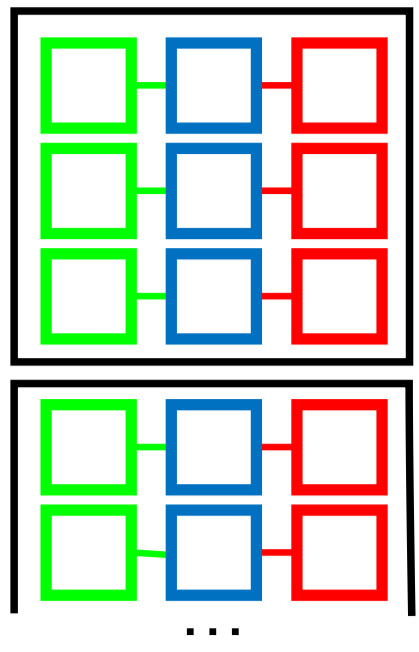
\includegraphics[width=100pt,height=120pt]{pictures/offline_triplet.jpg}
    \captionof{figure}{Minibatches in offline triplet mining. The green boxes are positive datapoints, the blue boxes are anchor datapoints and the red boxes are negative datapoints.\cite{siamese_leibe}}
    \label{fig:offline_triplet}
  \end{minipage}%
  \hspace{1cm}
  \begin{minipage}[t]{.45\textwidth}
    \centering
    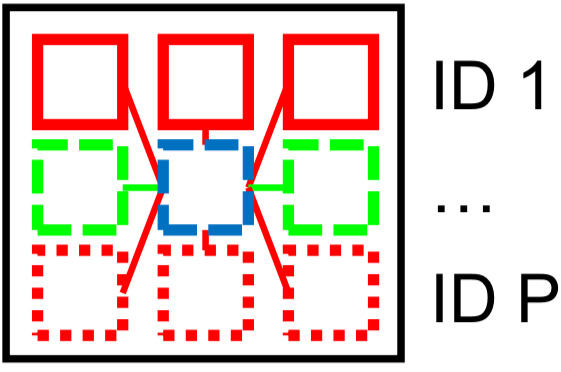
\includegraphics[width=100pt,height=120pt]{pictures/online_triplet.jpg}
    \captionof{figure}{Triplets constructed only within the minibatch. There are P object classes in the minibatch. The green boxes are positive datapoints, the blue boxe is the anchor datapoint and the red boxes are negative datapoints.\cite{siamese_leibe}}
    \label{fig:online_triplet}
  \end{minipage}
\end{figure}

\vspace{5mm}

\textbf{Triplet loss} function\cite{weinberger2009distance} trains the Siamese Network in a way that a triplet of datapoints are presented to the Siamese Network. By applying triplet loss the model tries to group the datapoints similar to the anchor datapoint, close to one another while increasing the distance between the anchor datapoint and the datapoints dissimilar to it as shown in Fig.\ref{fig:triplet_loss}. In order to do so, a positive value called margin is used which increases the distance between dissimilar datapoints and also eliminates the output of any trivial solution. Euclidean distance or cosine distance is used as the distance metric while calculating the triplet loss and shown in Eq. \ref{eq:triplet_loss}. \cite{hermans2017defense,siamese_network}
\begin{equation}
  \label{eq:triplet_loss}
  \mathcal{L}_{\textrm{tri}}(a,p,n)=\sum_{\substack{a,p,n \\ y_{a}=y_{p}!=y_{n}}} max(0,d(a,p)-d(a,n)+margin),
\end{equation}
where $y_{x}$ is the class label for the datapoint $x$ for $x \in \{a,p,n\}$, $a$ is the anchor datapoint, $p$ is the positive example having the same class label as the anchor datapoint and $n$ is the negative example having a different class label as compared to the anchor datapoint. But there are some practical problems related to the use of triplet loss function. The number of possible triplets grow cubically with the increase in the size of the dataset. Also most of the triplets are often uninformative. Thus, mining "hard triplets" or the ones crucial for the learning of the model becomes a challenging task. As per the definition of the triplet loss function, the triplets can be of three types: easy triplets, hard triplets and medium hard triplets. The triplets which satisfy the condition $d(a,p)+margin<d(a,n)$ results to the loss value being 0, hence are called the easy triplets\cite{triplet_loss}. For the triplet for which the negative datapoint is closer to the anchor as compared to the positive datapoint i.e. $d(a,n)<d(a,p)$ are the examples of hard triplets.\cite{triplet_loss} And the medium hard triplets are the ones where the negative datapoints are not closer to the anchor datapoint as compared to the positive datapoint but still results in positive loss i.e. $d(a,p)<d(a,n)<d(a,p)+margin$.\cite{triplet_loss} Thus, the medium hard triplets are the most essential for the model training as they constitute for the most useful information. Two triplet mining procedures are used to mitigate the issue of excessive computational overhead with increase in dataset size. They are offline triplet mining and online triplet mining. In offline hard triplet mining, at first the dataset is manually processed to find hard triplets and then they are used for training the model. But manually finding the hard triplets can be quite tedious. Online triplet mining is a better approach as compared to the one mentioned above. The model is trained in minibatches of the dataset as shown in Fig.\ref{fig:offline_triplet}. Using only the triplets that were mined from the dataset could be a wasteful design choice in such scenario. So in a minibatch, it contains way more potential triplets than the ones that were mined. So each member of another triplet becomes an additional negative datapoint example. But both hard positive and hard negative datapoints are required for training. An even better design to mitigate that would be to choose let's say $c$ datapoints from P different classes in the dataset, where the $k$ positive examples serve as hard positives while the rest of the datapoints in the minibatch serve as hard negatives as shown in Fig.\ref{fig:online_triplet}.\cite{hermans2017defense}

\vspace{5mm}

Thus, Siamese Networks are very robust to the class imbalance in dataset which is very common in real datasets. Since it depends on very few datapoints of a particular object class, it has good generalization capabilities for unseen datapoints in the future. They are also very robust to small perturbations in the datapoints due to difference in lighting conditions orientation or background, as they keep similar objects close to each other even if the datapoints are slightly different. Since the Siamese Networks places similar datapoints together while increasing the distance between dissimilar datapoints, they are often useful for learning semantic similarity within the datapoints. However despite its benefit, training a Siamese Network takes longer as compared to traditional neural networks because it involves learning from quadratic pair of datapoints.\cite{siamese_network, koch2015siamese}

\subsection{Clustering Algorithms}
\label{sec:Clustering_Algorithms}
\begin{figure}[t]
  \centering
  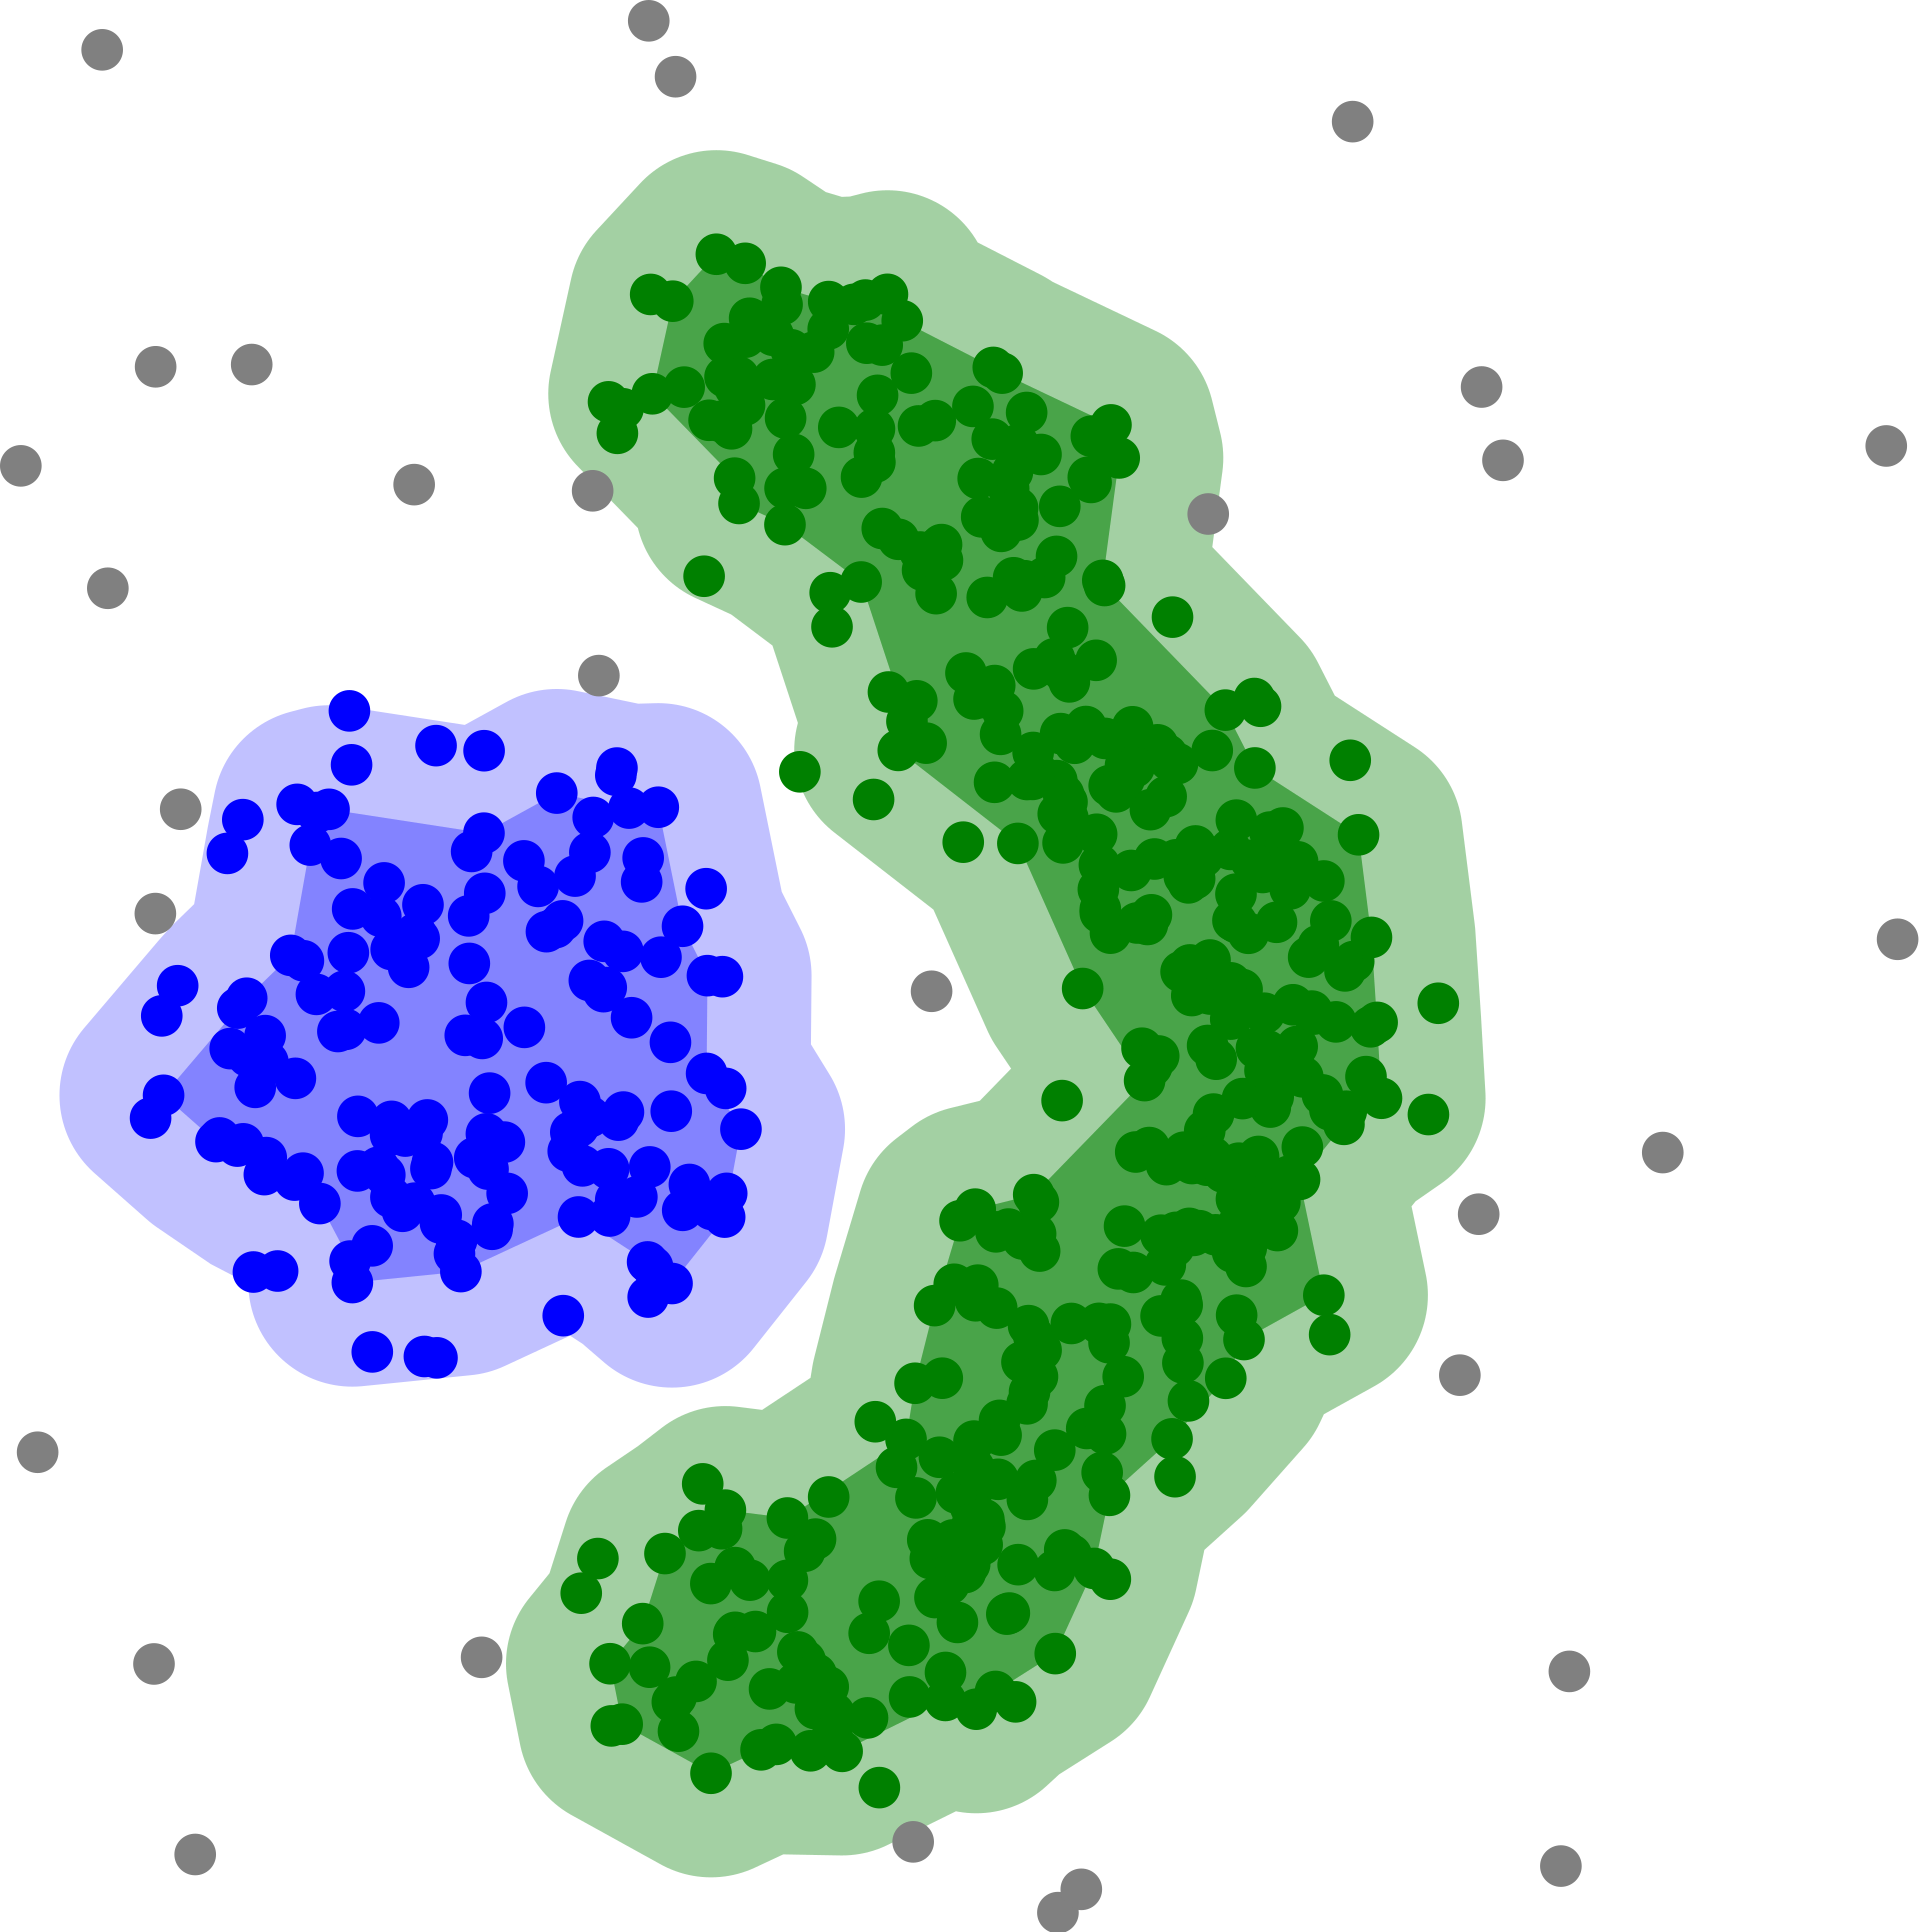
\includegraphics[width=200pt,height=150pt]{pictures/DBSCAN-density-data.png}
  \caption{\ac{DBSCAN} can find non-linearly separable non-convex clusters.\cite{dbscanWiki}}
  \label{fig:dbscan}
\end{figure} 
When the dataset does not have any labelled data, then it is said to be unsupervised learning. In this case, there is no ground truth available to measure the correctness of the outputs generated by the \ac{ML} models. The primary focus of unsupervised learning is to find hidden and interesting pattern in the data. Unsupervised learning is of utmost importance in the \ac{AI} world as several real world datasets do not have available annotations, which requires a lot of human effort. Unsupervised learning algorithms can be broadly categorized into the following: domains-clustering, dimensionality reduction and association analysis. Clustering algorithms aim at grouping unlabelled data into groups or clusters based on how similar or dissimilar the datapoints are to one another. It can reveal underlying hidden pattern in the data and is used in applications like image segmentation, fraud detection, etc. 

\vspace{5mm}

Dimensionality reduction reduces the number of irrelavant features or dimensions of the dataset. The inclusion of more features does help in the better representation of the dataset but it also significantly increases the memory consumption and complexity to work with it. Also it is often difficult to visualize real-life datasets with too many features. Association analysis is a rule-based unsupervised learning method that reveals the relationship between attributes in the dataset. It is used in applications like market analysis, intrusion detection, etc. Clustering algorithms can be broadly classified into the following categories: density-based, distribution-based, graph-theory based and hierarchical-based.\\
\begin{figure}
  \centering
  \begin{minipage}[t]{.45\textwidth}
    \centering
    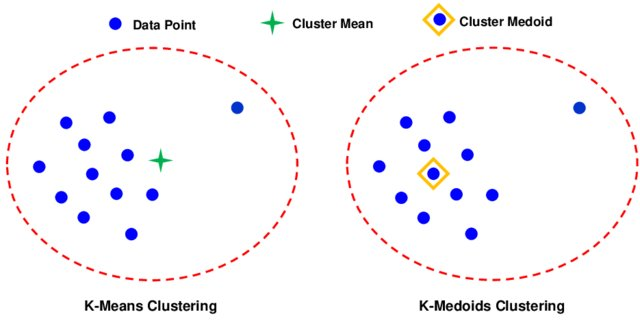
\includegraphics[width=200pt,height=150pt]{pictures/The-graphical-representation-of-the-difference-between-the-k-means-and-k-medoids_W640.jpg}
    \captionof{figure}{Difference between k-means and k-medoids.\cite{kmean-kmedoid}}
    \label{fig:kmean-kmedoid}
  \end{minipage}%
  \hspace{1cm}
  \begin{minipage}[t]{.45\textwidth}
    \centering
    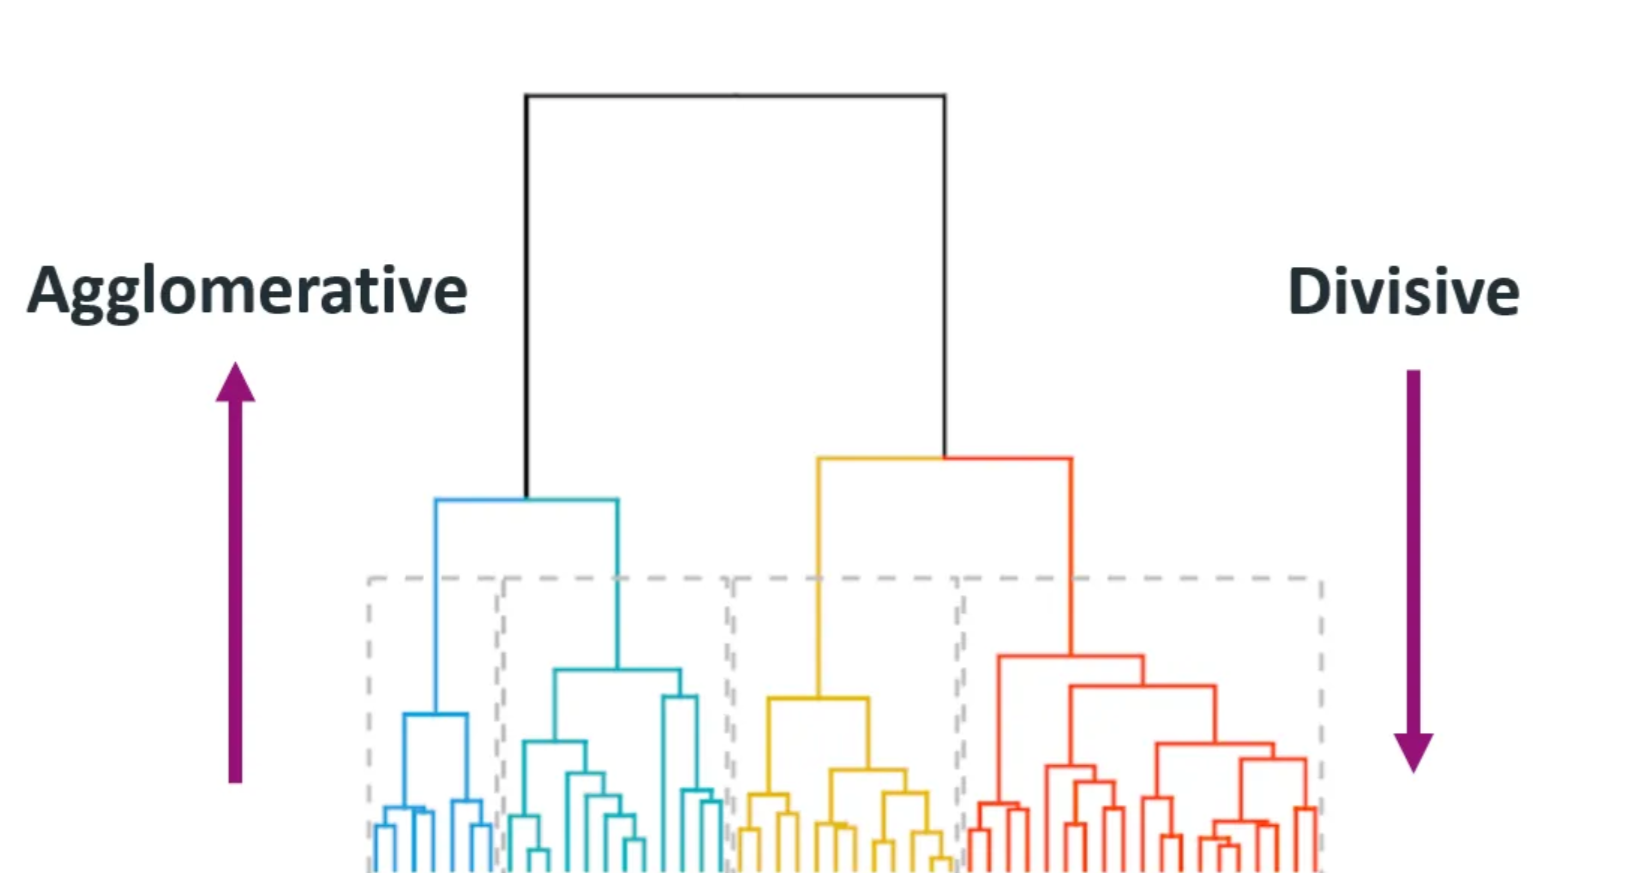
\includegraphics[width=200pt,height=150pt]{pictures/dendogram.png}
    \captionof{figure}{A dendogram in hierarchical clustering.\cite{dendogram}}
    \label{fig:dendogram}
  \end{minipage}
\end{figure}
\subsubsection{Density-Based Clustering}
 In density-based clustering, the algorithm looks for areas of high concentration of the datapoints and groups them as a cluster. The benefit of this algorithm is that the shape of a cluster is not limited and hence doesn't necessarily have to be convex in nature as show in Fig. \ref{fig:dbscan}.
Moreover, these algorithms are also very robust to outliers as they do not force the outliers to belong to any category but are rather ignored as it is unlikely that outliers can form an area of high concentration of datapoints. The experiments on this thesis have been carried on two such density-based clustering algorithms called \ac{DBSCAN}\cite{dbscan} and \ac{HDBSCAN} algorithms\cite{hdbscan}. The available scikit-learn python library implementations were used for this purpose\cite{scikit-learn}. The \ac{DBSCAN}\cite{dbscan} algorithm  does not require the users to define the number of clusters to be generated which doesn't force dissimilar datapoints to belong to the same cluster. However, this algorithm was still sensitive to two parameters $\epsilon$, the maximum distance between the datapoints to be considered in the same cluster and the minimum number of samples in the cluster which the user needs to define \cite{scikit-learn}. But finding an optimum value for these parameters often require domain expertise and are dependent on the data. The \ac{HDBSCAN}\cite{hdbscan} algorithm mitigates this issue and thus, does not require the user to define these two parameters. It is a hierarchical density-based clustering that performs the \ac{DBSCAN} algorithm over multiple $\epsilon$ values to find the most stable result. 

\subsubsection{Distribution-Based Clustering}
\label{sec:Distribution_based_Clustering}
In distribution-based algorithms, a datapoint is said to be a member of the cluster depending on the probability of its membership to the cluster. The more the distance of a point increases from the centre of the cluster, the less is its probability of belonging to that cluster. Centroid-based algorithms groups the datapoints based on some initial cluster centres. Once all the datapoints are softly assigned to some cluster membership, the cluster centres are recalculated and this process is iterated until convergence. These algorithms are sensitive to the initial parameters like the cluster centres chosen in the first step. Another major disadvantage of these clustering algorithms are that they always form spherical clusters. The user also needs to define the number of clusters the dataset is to be grouped in, which makes it sensitive to outliers. However, these algorithms can be executed very fast and two such algorithms were used during the experiments in this thesis- k-means\cite{kmeans}and k-medoids\cite{kmedoids}. In k-means, the mean of the datapoints of the clusters is assigned as the cluster-centroid. It might not be an actual datapoint in the dataset, rather a blurred, noisy average of a datapoints in the cluster. On the contrary, the k-medoids algorithm assigns an actual datapoint of the dataset, that is most centrally located as the cluster centroid as shown in Fig.\ref{fig:kmean-kmedoid}. Thus, k-medoids is more robust to outliers and noises as compared to k-means.\cite{arora2016analysis}

\subsubsection{Hierarchical-Based Clustering}
Hierarchical-based clustering algorithms form a hierarchy of clusters. Datapoints in a cluster are more similar to each other as compared to other groups. This hierarchy of clusters is visualized by a hierarchy tree called dendograms. Hierarchical clustering algorithms can be of two types - agglomerative and divisive. In agglomerative clustering, each datapoint is considered as a separate cluster in the first step. Then these clusters are merged into one another until only one cluster remains. Thus, at the end, the last level cluster consists of all the datapoints in the dataset. The divisive method is the reverse procedure of the agglomerative method. In the beginning, all the datapoints are considered to be in a single cluster and gradually the cluster is broken into smaller clusters, until each cluster consists of only one datapoint. A visual representation of a dendogram has been shown in Fig.\ref{fig:dendogram}.\cite{murtagh2012algorithms}

\subsubsection{Graph Theory-Based Clustering}
Spectral clustering is a powerful machine learning tool which divides datapoints into meaningful groups based on their similarity. The concept of spectral clustering has its root in the graph theory. It tries to determine the node communities in a graph by looking at the edges that connect them. It is specially useful when the dataset cannot be linearly-separated. The affinity matrix of the datapoints, which gauges the pairwise similarity between points, is the basis for spectral clustering. It works by creating a graph representation of the data, in which datapoints are represented by nodes and the degree of similarity between the points indicated by edges. After that the eigenvectors of a matrix is obtained from this graph which is used to create the embeddings of the datapoints in a lower dimensional space.  The embedded points are then divided into clusters by using a common clustering algorithm, usually the distributed based clustering algorithm k-means, where each entry in the embedding matrix is the representation of the datapoints in the lower dimensional space. Spectral clustering has shown promising results with datasts that have complex structures and non-linear separability, which makes it a useful tool in varity of fields, such as social network analysis, image segmentation and dimensionality reduction\cite{von2007tutorial}. A comparison between the results of k-means and spectral clustering in the presence of non-globular clusters in shown in Fig. \ref{fig:spectral}.\cite{demmel1999cs}
\begin{figure}[t]
  \centering
  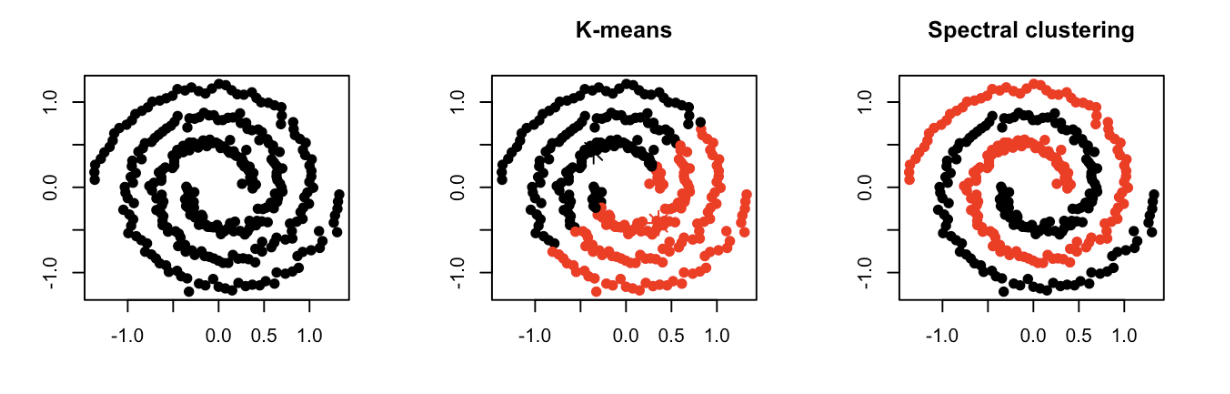
\includegraphics[width=400pt,height=200pt]{pictures/spectral.PNG}
  \caption{A comparison between the results of k-means clustering and spectral clustering. The image in the left shows the points that need to be clustered.\cite{palmer2021spectral}}
  \label{fig:spectral}
\end{figure} 

\subsection{Evaluation Metrics for Clustering Algorithms}
The ground truth or labels are available in supervised learning. So to determine the quality of the clustering algorithm the level of accuracy is calculated by comparing the labels predicted by a model to the ground truth. But most real world datasets do not have a ground truth. Therefore, it makes it challenging in unsupervised learning paradigm to determine the quality of the clustering algorithm. A good clustering algorithm is still expected to have little difference between the objects in a cluster i.e. small within-cluster variance and more difference between objects from different clusters i.e. large between-cluster variance. Thus, the evaluation metrics used in the literature could be categorized into two broad groups: extrinsic measures and intrinsic measures, depending on the availability of the ground truth. Extrinsic measures, when the ground truth is available uses metrices like Rand Index, Mutual Information, V-measure and Fowlkes-Mallows Scores. Intrinsic measures, when the ground truth is not available mostly uses Silhouette Score, Calinski Harabaz index and David Bouldin index.

\subsubsection{Silhouette Score}
Silhouette Score is used to calculate the distance between points within a cluster as compared to its distance from the points in the neighbouring cluster and is given by Eq. \ref{eq:silhouette_score}.
\begin{equation}
  \label{eq:silhouette_score}
  \mathit{S_{c}}= \mathit{\frac{(n_{c}-i_{c})}{max(n_{c},i_{c})}},
\end{equation}
where $S_{c}$ is the Silhouette Coefficient, $n_{c}$ is the average of the nearest-cluster distance of each datapoint and $i_{c}$ is the average distance between the datapoint within the cluster. The Silhouette coefficient lies within the range $[-1,1]$, where the the more closer the coefficient is to 1, the better is the clustering results. When the Silhouette Coefficient is close to 0, it implies that the datapoints are on or very close to the decision boundary between adjacent clusters, whereas negative values imply that the datapoints have been wrongly classified. But the drawbacks of using this metric is, that is tends to favour dense and convex clusters. Since it takes into account the average of the distance within a cluster as well as between adjacent clusters, it doesn't perform well if different clusters have a significant difference in their respective sizes, which is quite a common phenomenon in real world datasets. The chosen distance metric for the calculation of the Silhouette score also has a significant effect on it and can lead to very different results.

\subsubsection{Calinski-Harabasz Index}

Calinski-Harabasz Index(C-H Index) or the Variance Ratio Criterion is used to measure the dispersion between the datapoints within a cluster as compared to in-between clusters as in given by Eq. \ref{eq:c-h index}.
\begin{equation}
  \label{eq:c-h index}
  \mathit{S_{CH}}= \mathit{\frac{tr(B_{k})}{tr(W_{k})}} \times \mathit{\frac{(n_{E}-k)}{k-1}},
\end{equation}
where $S_{CH}$ is the C-H Index, $tr(B_{k})$ is the trace of the in-between cluster dispersion matrix. $B_{k}$ is in Eq. \ref{eq:Bk}  and $tr(W_{k})$ is the trace of the within-cluster dispersion matrix. $W_{k}$ is shown in Eq. \ref{eq:Wk}.
\begin{equation}
  \label{eq:Bk}
  \mathit{B_{k}}= \mathit{\sum_{q=1}^{k}n_{q}(c_{q}-c_{o})(c_{q}-c_{o})^T}, 
\end{equation}
\begin{equation}
  \label{eq:Wk}
  \mathit{W_{k}}= \mathit{\sum_{q=1}^{k}\sum_{x \in C_{q}}(x-c_{q})(x-c_{q})^T}, 
\end{equation}
where, $C_q$ is the collection of points in cluster $q$, $c_{q}$ is the centroid of the cluster $q$ and $c_{o}$ is the overall centroid of the datapoints. $B_{k}$ calculates the quality of the separation between two clusters, i.e. higher the value of $B_{k}$, better it is. $W_{k}$ calculates the distance of a datapoint ($x$) from the centroid of the cluster and thus, measures the cohesiveness or compactness of the datapoints within a cluster, i.e smaller the value of $W_{k}$ the better it is. Distribution-based clustering algorithms like k-means tries to minimize the value of $W_{k}$. Thus, according to the equation of C-H Index in Eq. \ref{eq:c-h index}, the higher the C-H index, the better is the clustering results. Because sum-of squared Euclidean distance is used to calculate the distance of the datapoints from their respective cluster centroids, C-H Index tends to favour convex clusters, which is a major drawback of using this metric similar to that in Silhouette Coefficient.\cite{chindex}

\subsubsection{David-Bouldin Index}

David-Bouldin Index is another metric used for evaluating clustering algorithms, which uses only the intrinsic features of the dataset and doesn't require any ground truth labels. David and Bouldin proposed R,a measure to calculate cluster similarity that satisfied the following conditions\cite{vergani2018soft}:
\begin{itemize}
  \item $R(S_i, S_j, M_{ij}) \geq 0$
  \item $R(S_i, S_j, M_{ij}) = R(Sj, S_i, M_{ij})$
  \item $R(S_i, S_j, M_{ij}) = 0$ iff $S_i = S_j$
  \item if $S_i = S_j$ and $M_{ij} < M_{ik}$, then $R(S_i, S_j,M_{ij}) > R(S_i, S_k,M_{ik})$  
  \item if $Mij = M_{ik}$ and $Sj > Si$, then $R(Si, Sj, M_{ij}) > R(Si, Sk, M_{ik})$
\end{itemize}
where $M_{ij}$ is the distance between the centroids of the clusters $i$ and $j$ and $S_i$ and $S_j$ are their respective dispersion measures. The conditions enforce that the cluster similarity measure R is non-negative and symmetrical in nature. It becomes 0 if and only if the dispersions of the two clusters disappear. If the distance $M_{ij}$ increases even if $S_i$, $S_j$ are constant, then the cluster similarity measure R decreases and vice versa. Also if $M_{ij}$ remains constant and $S_i$, $S_j$ increases, then R increases. Thus, the David-Bouldin Index was defined as the average of the similarities of each cluster as in Eq. \ref{eq:dbi}, using the same notations as the authors.
\begin{equation}
  \label{eq:dbi}
  \mathit{\bar{R}}= \mathit{\frac{1}{C}\sum_{i=1}^{C}R_i}, 
\end{equation}
where C is the total number of clusters and $R_i$ is the $max_{j \neq i}{R_{i,j}}$. Thus, $\bar{R}$ or the David-Bouldin Index is the average of the similarity measures R of each cluster with its most similar cluster. Thus, David-Bouldin Index has a lower bound of 0, while a higher value means bad clustering. In other words, the less is the average similarity, the better is the clustering results. Because of this, it acts as a good measure to decide on the number of clusters that actually exists in the dataset. Therefore, this index can be used to determine the number of clusters in distribution-based clustering algorithms like k-means. $R_{i,j}$ is more formally defined as in Eq. \ref{eq:ri}.
\begin{equation}
  \label{eq:ri}
  \mathit{R_{i,j}}= \mathit{\frac{S_i + S_j}{M_{ij}}}. 
\end{equation}
The dispersion measure of a cluster $i$ is defined by $S_I$ as in Eq. \ref{eq:si}.
\begin{equation}
  \label{eq:si}
  \mathit{S_i}= \mathit{\left\{\frac{1}{N_i}\sum_{j=1}^{N_i} \lVert X_j - A_i \rVert^q\right\}^{\frac{1}{q}}}, 
\end{equation}
where $N_i$ are the number of datapoints in the cluster $i$ and $X_j$ are the respective vector representations of the datapoints in the cluster $i$. For $q=1$, The dispersion measure $S_i$ is the average Euclidean distance of the vector representation of the datapoints from the centroid of the cluster $i$, while for $q=2$, it is the standard deviation of the metric about the datapoints in the cluster with respect to its centroid \cite{vergani2018soft}. It is different as compared to the distance defined between the centroids of the clusters which are defined as in Eq. \ref{eq:mij}.
\begin{equation}
  \label{eq:mij}
  \mathit{M_{i,j}}= \mathit{\left\{\sum_{k=1}^{N} \lVert a_{ki} - a_{kj}, \rVert^p\right\}^{\frac{1}{p}}} 
\end{equation}
where $a_{ki}$ is the k-th component of the vector representation of $a_i$ which is the centroid of the cluster $i$. $M_{i,j}$ is the Minkowski metric of the centroids of the clusters $i$ and $j$, i.e. when $p=1$, it is the Manhattan distance and when $p=2$ it is the euclidean distance between the centroids. When both p and q are 2, then $R_{i,j}$ is the Fisher similarity measure between the two clusters \cite{vergani2018soft}. But this metric too is not without its limitations. It is not robust to noise and outliers, thus, giving an incorrect sense of good clustering. This index too is biased towards spherical clusters with similar sizes, thereby making it inappropriate for many real world applications. Moreover, since it is a metric of the clustering results on a global level and gives no information about the individual clusters, even a single "too good" or "too bad" cluster can heavily influence the final result.

\subsection{Transfer Learning}
Transfer learning is an improvement in machine learning techniques where a model trained for a particular task. Let's say task 1 is different from another task, task 2. It uses the knowledge learnt by the model in the previous task to be adapted for the new task. Transfer learning has its benefits in a multitude of applications because real world problems doesn't necessarily always have an abundant amount of labelled data which can be used to train a model from scratch \cite{weiss2016survey}. It can be used for tasks which intend to solve different but related problems \cite{weiss2016survey}. In other words, if the domain of the data for task 2 is similar to that of task 1, transfer learning can be used as shown in Fig. \ref{fig:source_target}. Several approaches have been adapted to use transfer learning. Let's say one wants to solve task $T_{1}$ but don't have adequate data to train a deep neural network for it. But there is ample data to solve a similar task $T_{2}$. So one can train a model for task $T_{2}$ and then use it for task $T_{1}$. It might be needed to re-train only the later layers or all the layers of the model but that heavily depends on the problem at hand. Another approach that could be adapted is to use an existing pre-trained network. There are a lot of available open-source models which can be re-trained and re-used depending on the problem. Some of the popular models that are used as pre-trained models in transfer learning are Oxford VGG Model \cite{simonyan2014very},Google Inception model \cite{szegedy2015going} and Microsoft ResNet model \cite{he2016deep}. Another approach could be to use transfer learning for the purpose of feature extraction. Transfer learning has found a lot of application in the domain of computer vision and natural language processing because it requires a lot of data for training such complex models from scratch. In the domain of computer vision, it is known that the early layers of a deep neural network focuses on learning the low level features like the detection of edges, while the middle layers focus on learning the mid level features like the detection of shapes. In transfer learning, these pre-trained early and middle layers generally referred to as backbones could be used verbatim and only the latter layers which focus on the high level features could be re-trained for the new task as shown in fig \ref{fig:transfer_learning}.
\begin{figure}
  \centering
  \begin{minipage}[t]{.45\textwidth}
    \centering
    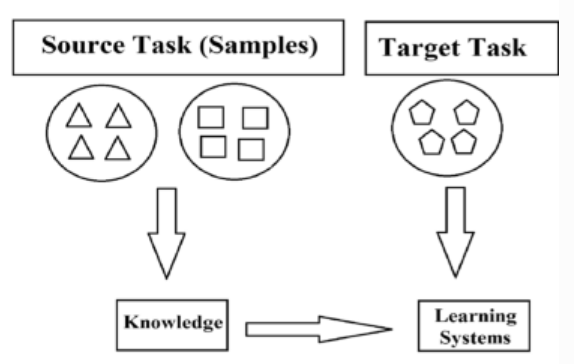
\includegraphics[width=100pt,height=120pt]{pictures/source_target.PNG}
    \captionof{figure}{Model trained for a task in the similar domain is re-used for a new task.\cite{hosna2022transfer}}
    \label{fig:source_target}
  \end{minipage}%
  \hspace{1cm}
  \begin{minipage}[t]{.45\textwidth}
    \centering
    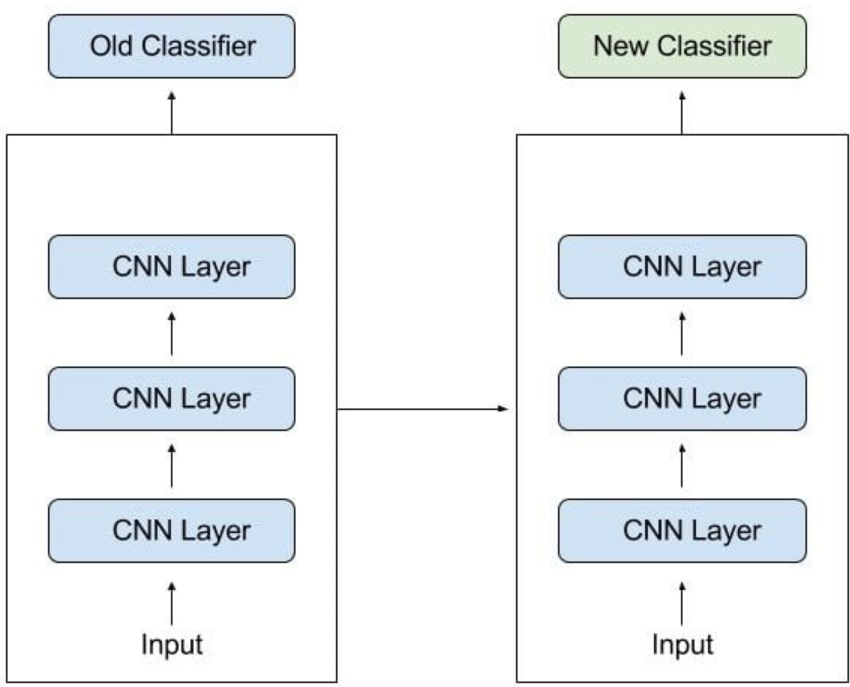
\includegraphics[width=100pt,height=120pt]{pictures/transfer_learning.PNG}
    \captionof{figure}{A model trained on a different task is adapted to be used for a new task.\cite{transfer_learning}}
    \label{fig:transfer_learning}
  \end{minipage}  
\end{figure}
Transfer learning has numerous advantages like significant reduction in the amount of training time\cite{liu2019exploring}, improvement in performance for some neural networks\cite{pan2011transfer} and less reliance on a huge amount of data\cite{duan2012learning,kulis2011you,zhu2011heterogeneous}.  
\subsubsection{Definition}
According to \cite{weiss2016survey,pan2009survey}, transfer learning can be formally defined as the following. A domain $\mathcal{D}$ of the input data, with the feature space $\mathcal{X}$ and a marginal probability distribution $P(X)$ such that $X=\{x_{1},.....,x_{n}\} \in \mathcal{X}$, where $n$ is the number of feature vectors in $X$. In the given input data domain $\mathcal{D}$, the task $\mathcal{T}$ has a label space $\mathcal{Y}$ and a predictive function $f(\cdot)$ which is learned from the feature vector and label pairs $(x_{i},y_{i})$ such that $x_{i} \in \mathcal{X}$ and $y_{i} \in \mathcal{Y}$ and $f(x)$ is the learner that predicts the label value for x. As per the above definition, the source domain is defined as $\mathcal{D_{\mathcal{S}}}$ and the corresponding source task as $\mathcal{T_{\mathcal{S}}}$.The target domain is defined as $\mathcal{D_{\mathcal{T}}}$ and the corresponding target task as $\mathcal{T_{\mathcal{T}}}$. Transfer learning aims at improving the target predictive function $f_{\mathcal{T}}(\cdot)$ by using the related information from $\mathcal{D_{\mathcal{S}}}$ and $\mathcal{T_{\mathcal{S}}}$ where $\mathcal{D_{\mathcal{S}}}\neq \mathcal{D_{\mathcal{T}}}$ or $\mathcal{T_{\mathcal{S}}}\neq \mathcal{T_{\mathcal{T}}}$. Since $\mathcal{D_{\mathcal{S}}} = \{\mathcal{X_{\mathcal{S}}},P(X_{\mathcal{S}})\}$ and $\mathcal{D_{\mathcal{T}}} = \{\mathcal{X_{\mathcal{T}}},P(X_{\mathcal{T}})\}$, here the condition $\mathcal{D_{\mathcal{S}}}\neq \mathcal{D_{\mathcal{T}}}$ means that $\mathcal{X_{\mathcal{S}}}\neq \mathcal{X_{\mathcal{T}}}$ and/or $P(X_{\mathcal{S}}) \neq P(X_{\mathcal{T}})$. The scenario where $\mathcal{X_{\mathcal{S}}}\neq \mathcal{X_{\mathcal{T}}}$ in the context of transfer learning is defined as heterogeneous transfer learning. The scenario where $\mathcal{X_{\mathcal{S}}} = \mathcal{X_{\mathcal{T}}}$ is defined as homogeneous transfer learning. The scenario where $P(X_{\mathcal{S}}) \neq P(X_{\mathcal{T}})$ means the source and the target data are from different domains, i.e. they belong to different marginal distributions. Transfer learning algorithms are not expected to give optimal results in ths case. Refering back to the definition of transfer learning, when $\mathcal{T_{\mathcal{S}}}\neq \mathcal{T_{\mathcal{T}}}$ and it was defined that $\mathcal{T} = \{\mathcal(Y),P(Y|X)\}$. This scenario is possible when $\mathcal{Y_{\mathcal{S}}} \neq \mathcal{Y_{\mathcal{T}}}$ and/or $P(Y_{\mathcal{S}}|X_{\mathcal{S}}) \neq P(Y_{\mathcal{T}}|X_{\mathcal{T}})$. The scenario where $P(Y_{\mathcal{S}}|X_{\mathcal{S}}) \neq P(Y_{\mathcal{T}}|X_{\mathcal{T}})$ implies that the conditional probability distributions between the source and target domains are different. The case $\mathcal{Y_{\mathcal{S}}} \neq \mathcal{Y_{\mathcal{T}}}$ means the label space of the source and target domain are different.\cite{weiss2016survey}
\subsubsection{Categories}
As per the definition of transfer learning mentioned above, it can be broadly categorized into 3 groups: inductive transfer learning, transductive transfer learning and unsupervised transfer learning as mentioned in \cite{pan2009survey}. Depending on the availability of labels of the source and target tasks, these 3 categories are possible as shown in Tab. \ref{tab:transfer_learning}.
\begin{table}[t]
  \centering
  \begin{tabular}{p{1.0in}|p{1.4in}|p{1.0in}|p{1.0in}|p{0.7in}}
  \toprule
    Transfer Learning Settings & Related Areas & Source Domain Labels & Target Domain Labels & Tasks \\\cline{1-5}
    \multirow{2}{1.0in}{Inductive Transfer Learning} & Multi-task learning & Available & Available & \multirow{3}{0.7in}{Regression, Classification} \\\cline{2-4}
    & Self-taught Learning & Unavailable & Available \\\cline{1-4}
    Transductive Transfer Learning & Domain Adaptation, Simple Selection bias, Co-variate Shift & Available & Unavailable \\\cline{1-5}
    Unsupervised Transfer Learning &  & Unavailable & Unavailable & Clustering, Dimensionality Reduction\\  
  \bottomrule    
  \end{tabular}
  \caption{Different settings of transfer learning.\cite{pan2009survey}}
  \label{tab:transfer_learning}
\end{table}
Regardless of whether the source and target domains are the same or not, the target task in an inductive transfer learning situation is distinct from the source task. In this instance, in order to generate an objective predictive function  $f_{\mathcal{T}}(\cdot)$ for usage in the target domain, some labeled data from the target domain are needed. Furthermore, inductive transfer learning can be broken down into two groups depending on the availability of source and target domain labels. When a lot of labeled data is available for the source domain, it is similar to multi-task learning. But the difference lies in the fact that the goal of inductive transfer learning is to attain good results in the target task only by using the knowledge obtained from the source task while multi-task learning endeavors to learn both the target and source tasks concurrently \cite{pan2009survey}. If the labels of the source data are not available, then it is similar to the self-taught learning as proposed by \cite{raina2007self}. In such a scenario, the label space of the source data and the target data can vary which means that the knowledge obtained from the source domain cannot be utilized directly. This implies that basically the labels of the source domain are not available.\cite{pan2009survey}

\vspace{5mm}

On the other hand, in transductive transfer learning, the target task and the source task are same but the source domain and the target domain are different. Depending on the similarity of the feature space and the marginal probability distribution between the source and the target domain, transductive transfer learning can be classified into two groups. One scenario can be that the feature space of the source domain and that of the target domain are different i.e. $\mathcal{X_{\mathcal{S}}} \neq \mathcal{X_{\mathcal{T}}}$. Again, the feature space of the two domains can be same but the  marginal probability distributions of the input data are different i.e. $P(X_{\mathcal{S}}) \neq P(X_{\mathcal{T}})$. Similar assumptions underlie the latter instance of the transductive transfer learning, which is related to sample selection bias \cite{zadrozny2004learning}, covariate shift \cite{shimodaira2000improving} and domain adaptation for knowledge transfer in text categorization \cite{daume2006domain,zadrozny2004learning}.\cite{pan2009survey}

\vspace{5mm}

Lastly, in unsupervised transfer learning, the target task is different from the source task as it was in inductive transfer learning but the labels of neither the source domain nor the target domain are available. The goal of unsupervised transfer learning is to solve unsupervised learning problems in the target domain like density estimation, dimensionality reduction and clustering\cite{dai2008self,wang2008transferred}. The categorisation of transfer learning has been summarised in Fig.\ref{fig:transfer_learning_overview}.
\begin{figure}[t]
  \centering
  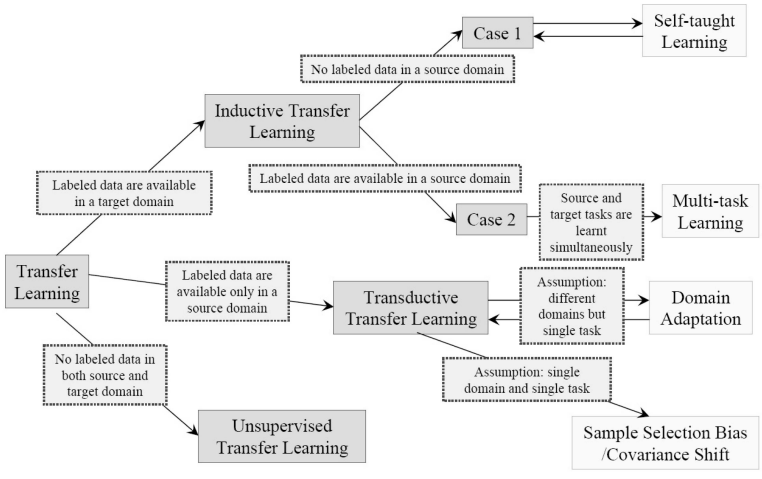
\includegraphics[width=350pt,height=200pt]{pictures/transfer_learning_types.PNG}
  \caption{Overview of the different types of transfer learning.\cite{pan2009survey}}
  \label{fig:transfer_learning_overview}
\end{figure} 

\subsection{Dimensionality Reduction}
Reducing the number of features (i.e. dimensions) in a dataset without sacrificing its relevant attributes is known as dimensionality reduction \cite{deng2022dimensionality}. This is equivalent to eliminating features that are superfluous, redundant or just noisy data, in order to build a model with fewer variables. Dimensionality reduction refers to a variety of preprocessing techniques for feature selection and data compression. Although dimensionality reduction techniques operate differently, they all use variable extraction or combination to convert high-dimensional spaces into low-dimensional spaces.\cite{deng2022dimensionality}

\vspace{5mm}

Dimensions, often known as features or input variables, are predictor variables in machine learning that control a model's output.  Any dataset having a significant number of predictor variables is regarded as high-dimensional data. Machine learning algorithms face several practical challenges when dealing with high-dimensional datasets, including longer calculation times and larger data storage requirements. Perhaps the greatest worry though, is that predictive models are becoming less accurate. Models in machine learning that are trained on high-dimensional datasets frequently have poor generalization.\cite{deng2022dimensionality}

\vspace{5mm}

\textbf{Curse of dimensionality} The inverse link between growing model dimensions and declining generalizability is known as the "curse of dimensionality". The model space rises with the amount of model input variables. Conversely, sparse data results from a constant amount of data points. This indicates that much of the feature space of the model is empty or devoid of observable data points. Data points get so different from one another as data sparsity rises that prediction models are less successful in finding explanatory patterns \cite{Goodfellow-et-al-2016}. Models may overfit on training data in order to explain patterns in sparse data sufficiently. Thus, poor generalizability may result from increases in dimensionality. By causing multicollinearity, high dimensionality might further impede model interpretability \cite{bellman46adaptive}. The effect of the number of model parameters on the performance of the model is shown in Fig. \ref{fig:dimensionality_reduction}.
\begin{figure}[t]
  \centering
  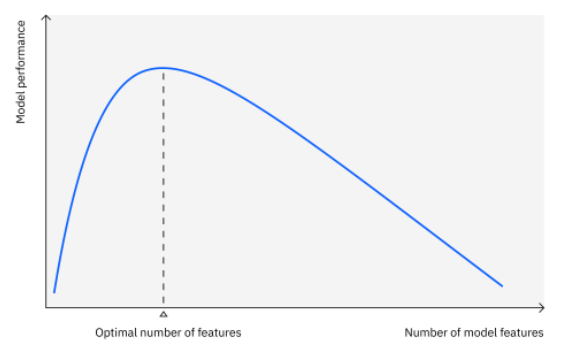
\includegraphics[width=350pt,height=200pt]{pictures/curse_of_dimensionality.PNG}
  \caption{The effect of the number of model parameters on the model performance.\cite{dr}}
  \label{fig:dimensionality_reduction}
\end{figure} 
 There is a chance that certain variables are unnecessary or associated as the number of model variables rises. The curse of dimensionality can be mitigated by increasing the collection of data by reducing data sparsity. However, the number of data points required to counteract the curse of dimensionality grows exponentially with the number of dimensions in a model. Its not always possible of course, to gather enough data. Therefore, dimensionality reduction is necessary to enhance data analysis. \ac{PCA}, \ac{LDA} and \ac{t-SNE} are dimensionality reduction algorithms that improve machine learning models.\cite{deng2022dimensionality}

\subsubsection{Linear Discriminant Analysis}
In supervised machine learning, \ac{LDA} is a method used to resolve multi-class classification problems. It reduces the dimensionality of the data to enable the separation of several classes with numerous features. A generative model framework is used in \ac{LDA}, which is often referred to as \ac{NDA} or \ac{DFA}. In other words, \ac{LDA} algorithms estimate the distribution of data for each class and classify additional data points by applying Bayes' Theorem \cite{bellman46adaptive}. Conditional probabilities or the likelihood of an event given the occurrence of another event are computed by Bayes Theorem. It is used by \ac{LDA} algorithms to determine the likelihood that a particular data item will be included in a specific output. Finding a linear feature combination that distinguishes any number of categories of objects or events is how \ac{LDA} operates. To facilitate easier classification, \ac{LDA} projects data with at least two dimensions into a single dimension as shown in Fig. \ref{fig:lda}. 
\begin{figure}[h]
  \centering
  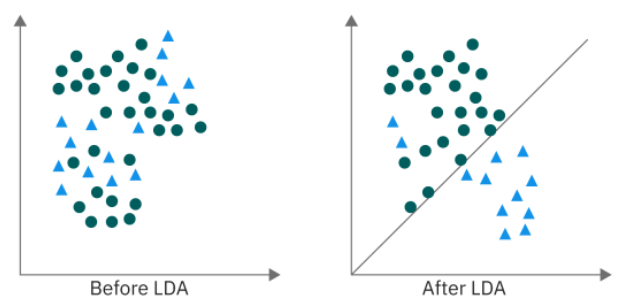
\includegraphics[width=300pt,height=200pt]{pictures/lda.PNG}
  \caption{Projection of the data before and after applying \ac{LDA}.\cite{dr}}
  \label{fig:lda}
\end{figure} 
As a result, the method is occasionally called "dimensionality reduction". Unlike logistic regression for example, which is restricted to binary classification, \ac{LDA}'s adaptability guarantees that it may be applied to multi-class data classification issues. For this reason, it is frequently used to improve the performance of other machine learning classification methods, such as \ac{SVM}, random forests and decision trees.\cite{xanthopoulos2013linear}

\subsubsection{Principal Component Analysis}
Similar to \ac{LDA}, \ac{PCA} is also a dimension reduction method. Unlike \ac{LDA}, it is not restricted to problems involving supervised learning. In other words, PCA can reduce dimensions for unsupervised learning tasks without taking class labels or categories into account. Mathematician Karl Pearson first presented the \ac{PCA} approach in 1901 \cite{sanguansat2012principal}. It functions under the requirement that the variance of the data in the space of fewer dimensions should be maximal even when data in a space with more dimensions is transformed to data in a lower dimensional space as shown in Fig. \ref{fig:pca}. In an unsupervised learning paradigm it can find the correlation between different features in the dataset.
\begin{figure}[t]
  \centering
  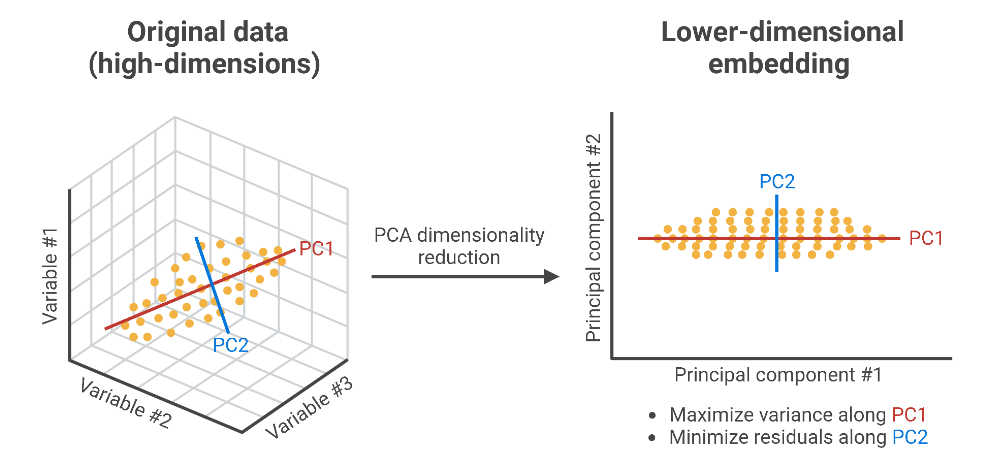
\includegraphics[width=350pt,height=200pt]{pictures/pca.PNG}
  \caption{Projection of the data from higher dimensional space to lower dimensional space on applying \ac{PCA}\cite{pca}}
  \label{fig:pca}
\end{figure} 
A linear combination of the the variables in the original dataset gives rise to the principal components.  By combining the variables in this manner, the majority of the information found in the original variables is condensed into the first components and these new variables or principal components are left uncorrelated. The premise is that ten-dimensional data sets provide ten principal components. PCA then attempts to assign the maximum amount of information to the first principal component, the maximum amount of information left to the second principal component and so on, until the result is somewhat like the Fig. \ref{fig:pca_variables}. By removing the components with little information and using the ones that remain as the new variables, the dimensionality can be minimized without compromising much information when the data is organized using principle components. Its crucial to understand that the primary components are created as linear combinations of the original variables, they are less interpretable and have no true significance. From a geometric perspective, the principal components are the data's directions that account for the greatest amount of variance or the lines that encompass the majority of the data's information. Here, variation and information are related in that a line's variance indicates how dispersed the data points are along it. The more dispersion a line has, the more data it contains. To put all of this into perspective, principle components are new vectors that offer the optimal viewpoint for examining and assessing the data, making the variations between the observations easier to observe.\cite{abdi2010principal} 

\vspace{5mm}

\textbf{Working priniciple for \ac{PCA}}\\
\begin{figure}[t] 
  \centering
  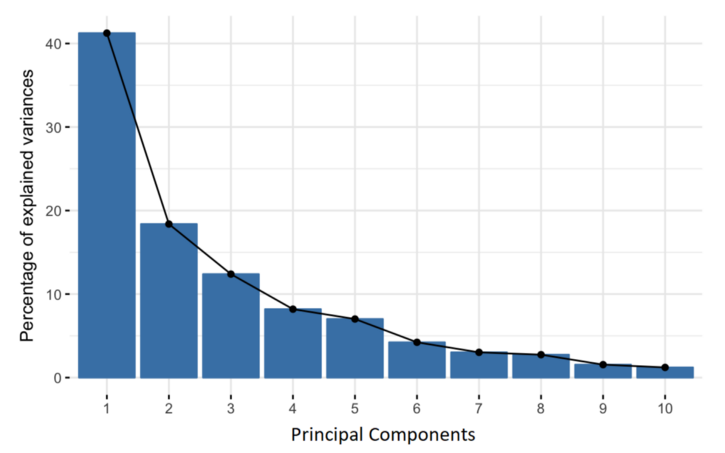
\includegraphics[width=350pt,height=200pt]{pictures/pca_variables.PNG}
  \caption{The percentage of explained variance for each principal component}
  \label{fig:pca_variables}
\end{figure}

\begin{enumerate}
  \item \textbf{Normalization} This step's objective is to normalize the continuous original variable's range to ensure each one makes an equal contribution to the analysis. More precisely, the reason \ac{PCA} is extremely sensitive to the variances of the original variables is because normalization must be done first. In other words, if the ranges of the initial variables differ significantly, the variables with greater ranges will take precedence over the variables with smaller ranges, which will produce biased results. Therefore, this issue can be avoided by translating the data to similar scales. The mathematical procedure for achieving this is to take each variable's value, subtract the mean and then divide the result by the standard deviation as shown in Eq. \ref{eq:norm}.
  \begin{equation}
    \label{eq:norm}
    \mathit{z} = \mathit{\frac{value-mean}{standard deviation}}.
  \end{equation}
  All of these variables will be converted to the same scale after standardization is complete.
  \item \textbf{Computation of covariance matrix} This step's objective is to determine whether there is a correlation between the variables in the dataset being analyzed and how they differ from the mean in relation to one another. Because variables might occasionally include redundant information due to strong correlations, the matrix of covariance is calculated to find these correlations. The correlation matrix of a 3-D data with variables $a$, $b$, $c$ are given by the covariance matrix shown below.\cite{abdi2010principal}
\begin{equation}
  \label{eq:cov_mat}
    \begin{bmatrix}
    Cov(a,a) & Cov(a,b) & Cov(a,c)\\
    Cov(b,a) & Cov(a,b) & Cov(a,c)\\
    Cov(c,a) & Cov(a,b) & Cov(a,c)
  \end{bmatrix}
\end{equation}
  The covariance matrix has all possible pairs of initial variables as entries and is a p × p symmetric matrix (where p is the number of dimensions).
  The variances of each starting variable are along the major diagonal (top left to bottom right), as the variance of a variable with itself is its covariance $(Cov(a,a)=Var(a))$. Furthermore, because the covariance is commutative $(Cov(a,b)=Cov(b,a))$, the covariance matrix's entries are symmetric with regard to the main diagonal, meaning that the top and lower triangular sections are equal. When two variables increase or decrease at the same time, i.e. they are correlated, then the value in the covariance matrix is positive. Whereas, if the two variables doesn't follow the same trend, i.e. one increases while the other decreases, then the variables are uncorrelated.\cite{abdi2010principal}
  \item \textbf{Computation of eigenvectors and eigenvalues} The two necessary mathematical concepts that are essential for the computation of the principal components are eigenvectors and eigenvalues. Every eigenvector has an associated eigenvalue with it. The number of eigenvectors or eigenvalues for the data is equivalent to the dimension of the data. The eigenvector gives the direction of the axis along which most of the variance of the original dataset is preserved or in other words the direction of the principal components. The eigenvalue associated with the eigenvector is the coefficient of the eigenvector, i.e. the amount of variance that particular principal component is responsible for in the total variance. The principal components are obtained by arranging the eigenvectors from highest to lowest of their corresponsing eigenvalues.\cite{abdi2010principal} 
  \item \textbf{Creation of feature vector} Creating the feature vector involves selecting which elements to keep and which to remove. Generally speaking, components with low eigenvalues won't be as important. A plot is generated to display the cumulative proportion of variation as well as the percentage of total variance. Typically, the number of PCA components that is to be included is indicated by the point at which the Y axis of eigenvalues or total variance forms a "elbow".\cite{abdi2010principal}
  \item \textbf{Data transformation along the axis of principal components} With the exception of normalization, none of the data is altered in the preceding steps. Instead, the input data set is always expressed in terms of the original axes or the original variables. The primary components are chosen and the feature vector is created. The goal of this final step is to reorient the data from the original axis to that of the principal components, thus, the name Principal Components Analysis represent by utilizing the feature vector that was created using the eigenvectors of the covariance matrix. To accomplish this, the feature vector's transpose is multiplied by the original data set's transpose as shown in Eq. \ref{eq:trans_data}.\cite{abdi2010principal}
  \begin{equation}
    \label{eq:trans_data}
    \mathit{TransformedDataSet} = \mathit{FeatureVector^T \times NormalizedOriginalDataSet^T}.
  \end{equation}
\end{enumerate}
\cleardoublepage


\section{Method}
\label{sec:method}
This chapter gives the details of the network, clustering algorithms and the evaluation metrics that are utilized and examined in this thesis. 
\subsection{Network}
\subsubsection{Selection of network}
The unsupervised feature representation learning approach proposed by Guofeng Mei \textit{et. al.}\cite{mei2022unsupervised} is adapted to be used in the existing scenario at \ac{IPA}. The primary motivation behind using an unsupervised learning  methodology is that annotation of point clouds can be really challenging. To really focus on the point level features of a point cloud, it is required to have a high number of points in the point cloud. And labelling such high number of points in each point cloud in large real world datasets can be really expensive and severely inefficient. Unsupervised learning facilitates high quality feature representation without the need for humans in the loop. Moreover, sporadic and non-uniform distribution of the point clouds can also add further challenges in point-level annotation of the point clouds. Thus, in the absence of such annotations, it is impossible to get supervised feature representations for computer vision tasks.\cite{mei2022unsupervised} 

\vspace{5 mm}

An unsupervised learning approach "ConClu" is proposed in \cite{mei2022unsupervised} that learns both the local features as well as the global features of the point clouds. It is suitable to be used in this scenario, as it would require no point-level annotation of the dataset, which is unavailable in this case. To do so, it performed point-level clustering of the points clouds to generate semantically related regions within the point cloud and performed instance-level contrasting to make the network robust to its global appearance which would be explained in detail in the following subsections.\cite{mei2022unsupervised}. Other related works like \cite{zhu2016deep} also worked in the domain of learning object feature representations using autoencoders but depth images were used in such cases. \cite{mei2022unsupervised} on the other hand worked with point clouds which is similar to the ABC dataset used at \ac{IPA}. Furthermore, as mentioned in the Ch. \ref{sec:related_works}, discriminative models have the capability of distinguishing between different data augmentations. Amongst them \cite{rao2020global} and \cite{sanghi2020info3d} is seen to have promising results because of the use of contrastive learning techniques. But it is computationally expensive generate negative samples required in contrastive learning in unsupervised learning. On the other hand, the mechanism of learning the global features which encapsulate the high-level semantic information reduces the necessity to rely on negative samples of contrastive learning. Therefore, the network used in \cite{mei2022unsupervised} is deemed suitable for the task in hand.\cite{mei2022unsupervised}


\subsubsection{Architecture}
Analysing how humans perceive an object, they do not focus merely on the individual points but rather semantically related points that form a group and act as the fundamental block for the entire object as a whole. The global features focus on the entire shape of the object while the local features attains to the more detailed information in the different parts of the object. In this work, the 3D point cloud $\mathcal{\textbf{P}} = \{\textbf{p}_i \in \mathbb{R}^3| i= 1,2,3,....,N\}$, where $N$ is the number of points in each point cloud and $\textbf{p}_i$ is each point in the point cloud representated in 3D cartesian coordinate system. The point cloud $\mathcal{\textbf{P}}$ is fed to an encoder backbone $f_{\varphi}$ which generates a point-wise feature matrix $\mathcal{\textbf{F}} = \{ f_{p_i}\}_{i=1}^{N}$ where $f_{p_i}$ is the point-wise feature vector. The objective is to train a feature encoder $f_{\varphi}$, PointNet in this case, having parameters $\varphi$ in an unsupervised learning paradigm. The entire pipeline of the process is elaborated in Fig.\ref{fig:conclu_arch}.
\begin{figure}[h]
    \centering
    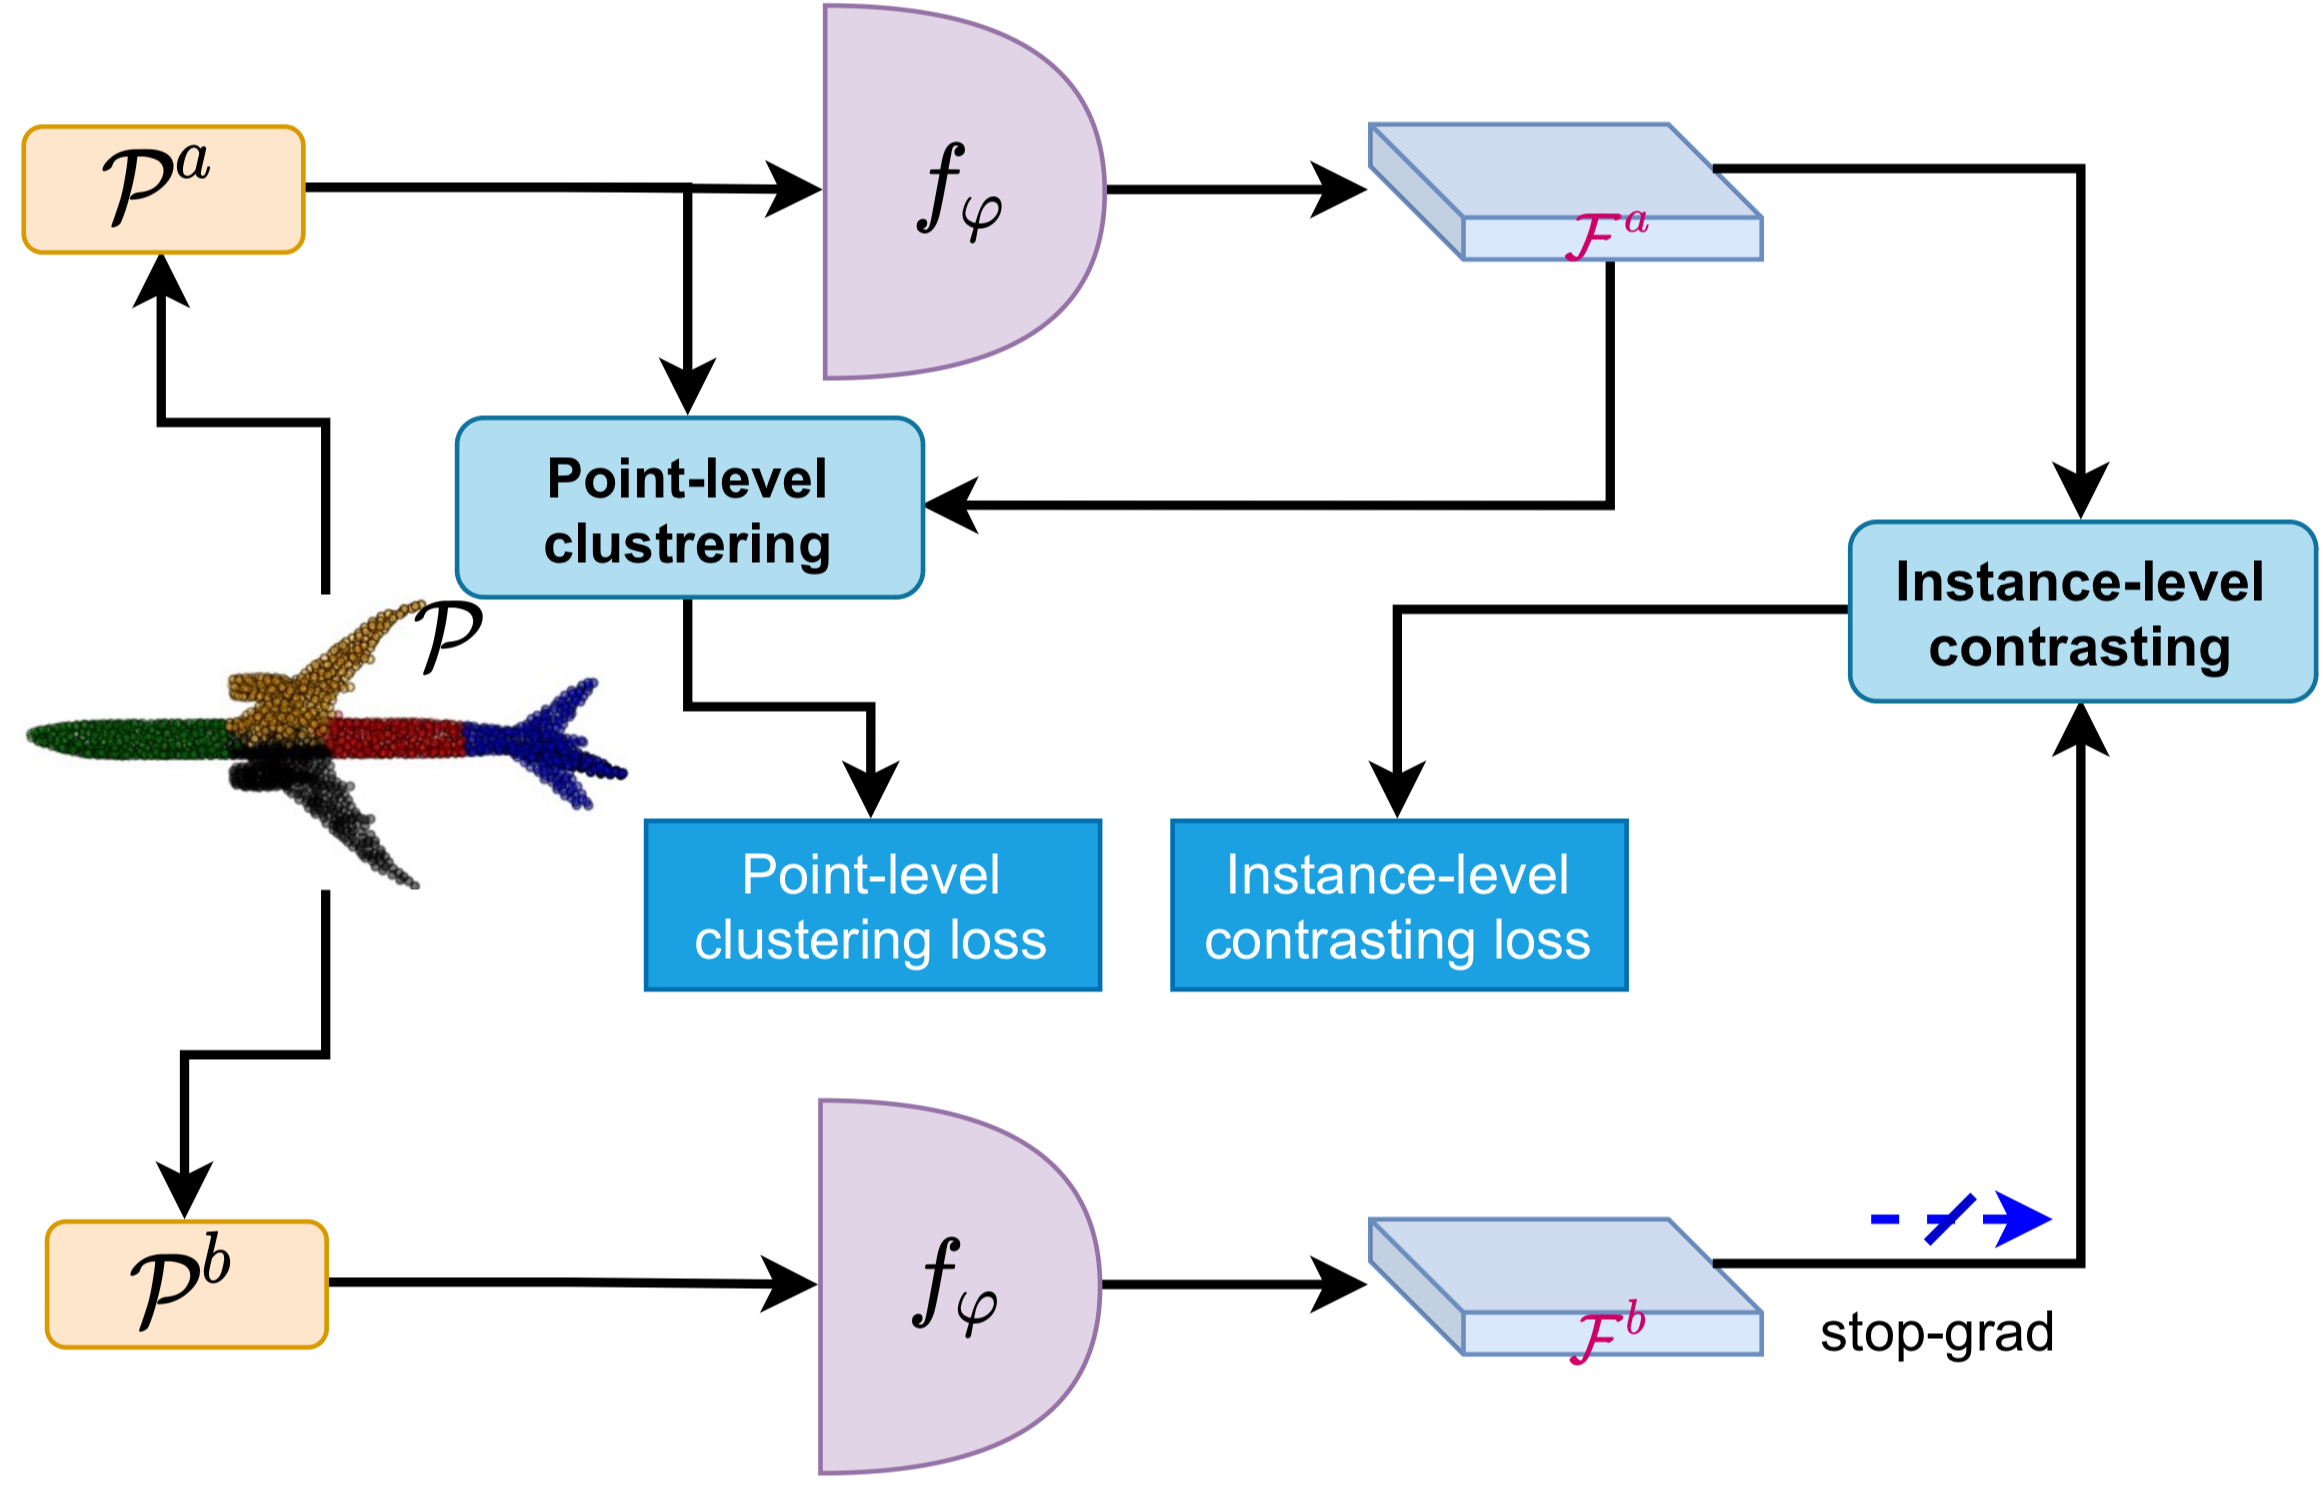
\includegraphics[width=320pt,height=200pt]{pictures/conclu_arch.jpg}
    \caption{The ConClu model pipeline including the two modules: point -level clustering and instance-level contrasting.\cite{mei2022unsupervised}}
    \label{fig:conclu_arch}
\end{figure} 
 As it can be seen that the architecture has two main parts: the point-level clustering for learning the local features and the instance-level contrasting for learning the global features. Before a detailed analysis of each module is given, here is a brief overview of the entire process. The augmented views $\mathcal{\textbf{P}}^a$ and $\mathcal{\textbf{P}}^b$ are obtained for each point cloud $\mathcal{\textbf{P}}$ and are fed to the encoder $f_{\varphi}$ such that it generates the feature matrices $\mathcal{\textbf{F}}^a$ and $\mathcal{\textbf{F}}^b$ respectively. Thus, the inputs to the point-level clustering are $\mathcal{\textbf{P}}^a$ and $\mathcal{\textbf{F}}^a$. It is to be noted here that the feature encoder $f_{\varphi}$ shares the weights between the two augmented views. $f_{\varphi}$ is trained in a way such that it minimizes the point-level clustering and the instance-level contrasting loss together. It is also to be noted here, that the encoder receives the gradient only from the top branch. After the training is completed, both the loses are cast aside and only the encoder is needed for further tasks.\cite{mei2022unsupervised}

\subsubsection{Encoder Backbone}
Keeping in line with \cite{mei2022unsupervised}, two feature representation learning backbones are used for the experiments, the PointNet \cite{qi2017pointnet} and the \ac{DGCNN} \cite{wang2019dynamic} backbone. The mechanism and the architecture of the feature extraction backbones are elaborated further in the following sections.
\subsubsection*{PointNet Autoencoder}

For the purpose of weight sharing and other kernel optimization methods, traditional convolution networks need extremely regular formats for the input data as prevalent in \ac{RGB} or depth images and 3D voxels. But point clouds are not regular data structures. It is just a set of 3D points which is permutation invariant to its constituent points. Or in other words, the order in which the individual points of a point cloud are processed is inconsequential. In \cite{qi2017pointnet} the authors suggested an end-to-end architecture that accepts the point clouds as input and generates the class label of the entire object or a class label for each of the individual points in the point cloud. The PointNet architecture is shown in Fig. \ref{fig:pointnet_arch}.
\begin{figure}[t]
    \centering
    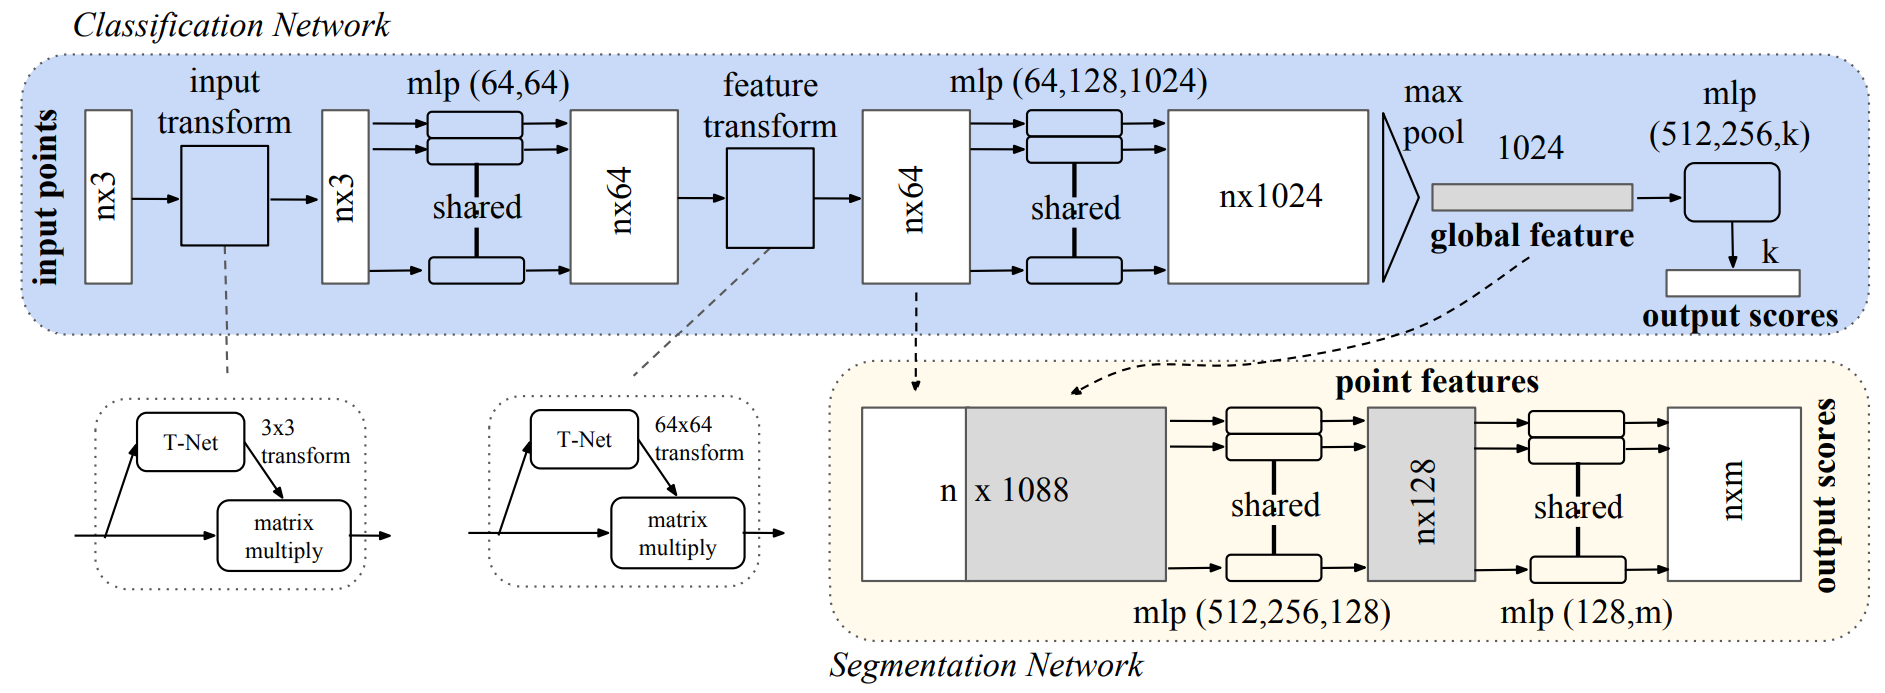
\includegraphics[width=400pt,height=250pt]{pictures/PointNet.png}
    \caption{The PointNet Architecture.\cite{qi2017pointnet}}
    \label{fig:pointnet_arch}
\end{figure}
It consists of three important modules:
\begin{itemize}
    \item a symmetric function to aggregate information, 
    \item a module that integrates the local and the global features, 
    \item an alignment network that orients the points of the point cloud and their features. 
\end{itemize}
A further detailed overview of each of the building blocks are given in the following passages.

\vspace{5mm}

\textbf{Symmetry function} The points in the point cloud are an unordered set of points, which means the order in which they appear is irrelevant. Therefore, to make the network invariant to permutation, the following approaches could be adopted. 
\begin{itemize}
    \item The input points could be sorted in canonical manner. Sorting the points isn't an efficient solution because in high dimension space there isn't actually any stable ordering w.r.t the point perturbations. Contradiction is a simple way to demonstrate that. If such an ordering existed, it would mean there is a bijection mapping between the higher dimension space and a 1d real line. For this ordering to be stable, the bijection mapping would need to maintain spatial proximity even if the dimensions decreased in the event of point perturbations. This is not feasible in most cases. As a result, sorting only partially fixes the ordering problem and it brings additional challenges for the network to learn a consistent bijection mapping between the input and the output.\cite{mei2022unsupervised}
    \item The second approach is to treat the points as a sequential data and training a \ac{RNN} with different randomly permuted input sequence in order to make it invariant to the order in which the input appears. But in \cite{vinyals2015order} it is proved that the order indeed matters and cannot be overlooked completely. Moreover, even if a \ac{RNN} is robust to the order of the input with small length(e.g. dozens), it suffers from scalibility issues. It can't be scaled to inputs with high number of elements as it is in point clouds.\cite{mei2022unsupervised}
    \item The data from each point could be combined using a symmetric function. Binary addition and multiplication are some examples of symmetric functions. Hence, the idea proposed by the authors in \cite{qi2017pointnet} is to devise a symmetric function on the transformed set of points to approximate the general function defined on the points as in Eq. \ref{eq:sym_func}.\cite{mei2022unsupervised}
\end{itemize}
   
\begin{equation}
    \label{eq:sym_func}
    f(\{x_1, ...., x_n\}) \sim g(h(x_1), ...., h(x_n)),
\end{equation}
where $\mathit{f}: 2_{\mathbb{R}_{\mathit{N}} \rightarrow \mathbb{R}}, \mathbb{R}^{\mathit{N}} \rightarrow \mathbb{R}^{\mathit{K}}$ and $g: \underbrace{\mathbb{R}^{\mathit{K}} \times ... \times \mathbb{R}^{\mathit{K}}}_\text{n} \rightarrow \mathbb{R}$ is the symmetric function. Here $h$ is a multi-layer perceptron network and $g$ is a combination of a single variable function and a max pooling function. Even if this module is fairly simple, it has some of the very important implications. If $\mathit{C_S}$ is the set of critical points, the points which contributed to the max pooled feature, the PointNet architecture is seen to be quite robust to the non-critical points. In other words, discarding the non-critical points don't lead to any loss of information about the global shape of the object as shown in Fig. \ref{fig:critical_points}. 

\begin{figure}[t]
    \centering
    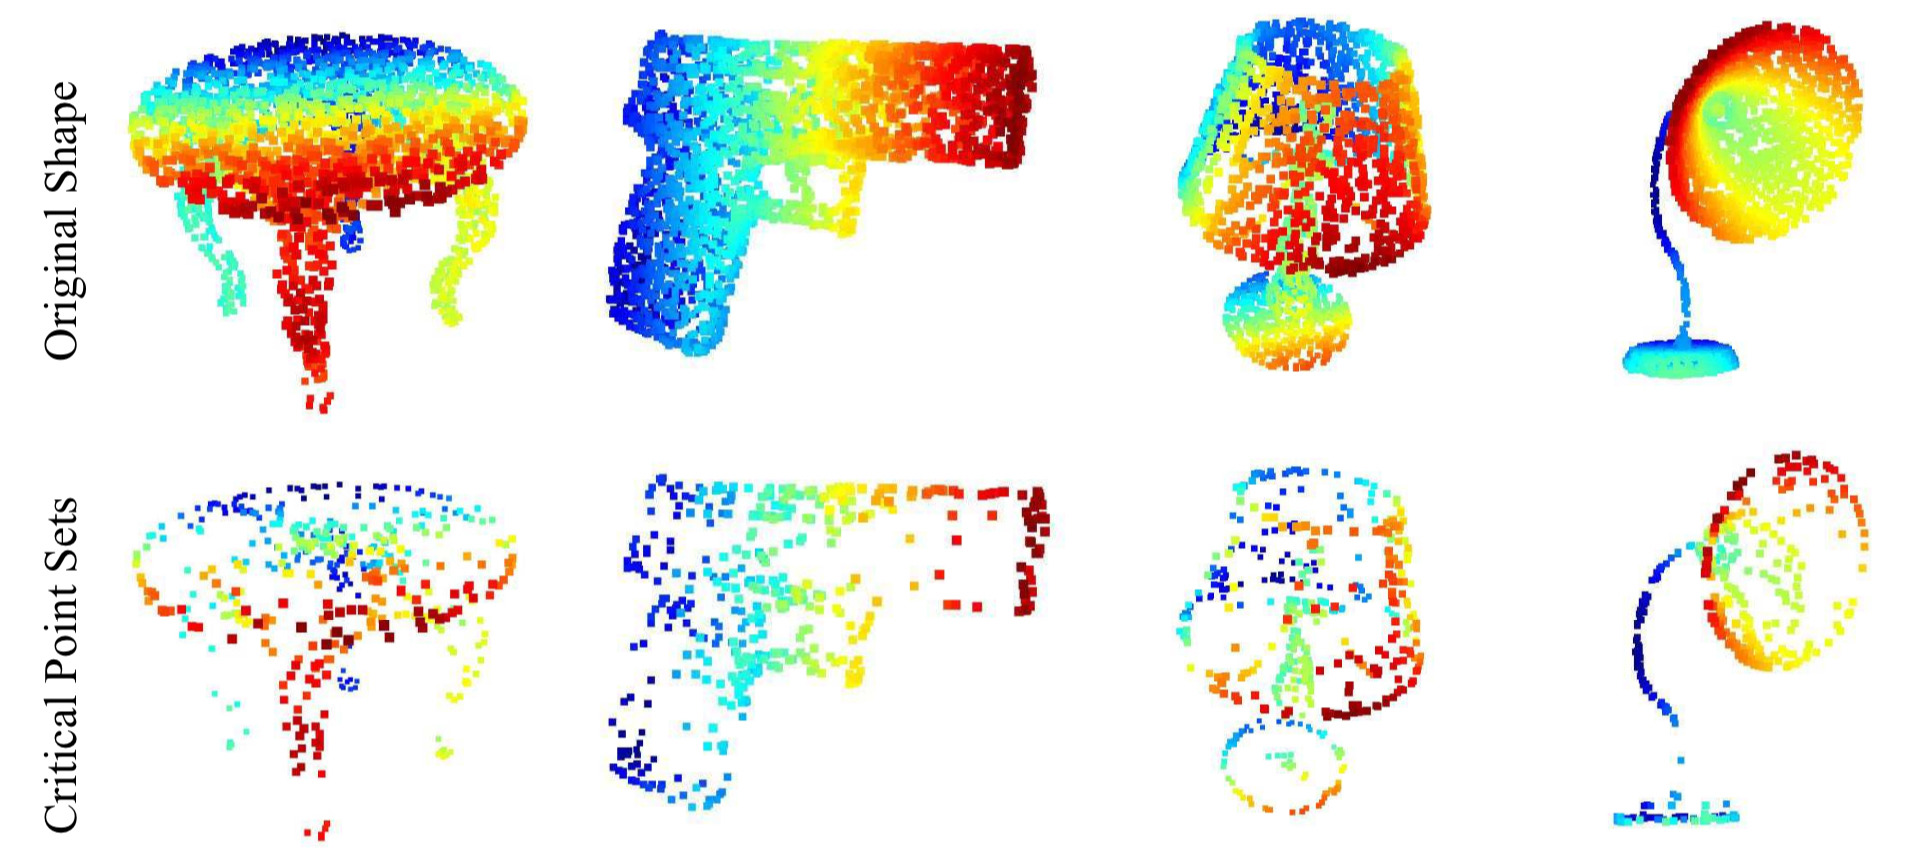
\includegraphics[width=300pt,height=150pt]{pictures/critical_points.jpg}
    \caption{Critical points set and the original shape.\cite{qi2017pointnet}}
    \label{fig:critical_points}
\end{figure}

\vspace{5mm}

\textbf{Local and Global Information Aggregation} The output of the symmetry function is a vector $[\mathit{f_1, ... , f_K}]$ which is the global feature representation of the point cloud. But to get a point-wise segmentation, information about both the local features and the global features are necessary. The local features are learnt by the network in the \textit{Segmentation Network} module as shown in Fig. \ref{fig:pointnet_arch}. Once the global feature vector of the point cloud is calculated, it is concatenated with each of the point features and is fed into the network. This enables the network to learn new point-level features when it is informed about both the local and the global information. Because of this module, the network is able to predict the class probability of individual point based on both the local geometry of the object as well as the semantic region it belongs to on a global-level.\cite{qi2017pointnet}

\vspace{5mm}

\textbf{Joint Alignment Network} The network should be invariant to certain geometric transformations like rigid body transformations. A trivial solution to this issue is aligning every input set to a canonical order prior to feature extraction. But this would require an additional layers for aligning all input sets. On the contrary, the authors in \cite{qi2017pointnet} utilized a "mini-network" (\textit{T-net}) as shown in Fig. \ref{fig:pointnet_arch}. This predicts a transformation matrix which is then applied to the coordinates of the points in the point cloud. The mini-network takes after the main network and is made up of point independent feature extraction module, max pooling layers and the fully connected layers. To align the point-features from different point cloud sets, another alignment network could be introduced. It would predict the transformation matrix required for the alignment. But that would significantly increase the difficulty of optimization since the transformation matrix has much higher dimensions as compared to the spatial transformation matrix. To circumvent this issue, a regularization term is used in the softmax training loss. The constraint enforced in this case is that the feature transformation matrix is to be approximated by an orthogonal matrix as given in Eq. \ref{eq:loss_reg}.
\begin{equation}
    \label{eq:loss_reg}
    L_{reg} = \lVert I - AA_T \rVert _F^2,
\end{equation}
where $\lVert . \rVert _F$ is the Frobenius-norm, $I$ is the Identity matrix and $A$ is the feature alignment matrix predicted by the mini-network. The feature transformation matrix has been approximated by an orthogonal matrix because orthogonal transformations ensure that no information about the input is lost.

\subsubsection*{Dynamic Graph Convolutional Neural Network}
Another more general feature encoder is used in this work. It is seen that the PointNet architecture treated each point of the point cloud independently. The model is made invariant to the different possible permutations by applying a symmetric function to aggregate the features. But a limitation to this method is that it doesn't take into consideration the topology of the points. It ignores the connectedness in between the points and thus, cannot learn the local features. This limitation is addressed by Y. Wang \textit{et al.} in \cite{wang2019dynamic}. The authors proposed the EdgeConv operation which is able to learn the local features of the point cloud while still meeting the requirement of being permutation invariant. EdgeConv generated the edge features which are capable of capturing the topological information of the points i.e. the connection between a point and its neighbors. In other words, the EdgeConv operation computes a local graph for each of the points in the point cloud which is capable of learning the edge embeddings for the edges in the graph. So the model group points based on both the Euclidean distance between the points and also how they are semantically related. The EdgeConv is a plug-and-play module that would be used combined into any existing model architecture to further enhance its performance. The approach has been further elaborated in the following passages.

\vspace{5mm}

Unlike PointNet, the \ac{DGCNN} network captures the topological information by generating a local neighborhood graph and then applying an operation analogous to the convolution operation on the edges connecting a pair of points. It is in line to the methodology used in graph neural networks. But unlike a traditional graph \ac{CNN}, the local neighborhood graph is not fixed in this case. On the contrary, it is updated after every layer in the network. This is because the k-nearest neighbors of a point doesn't remain the same after every layer of the network. This happens as the k-nearest neighbors are based on the Euclidean distance between the points but rather of the proximity of the points based on the learnt embeddings. In other words, the proximity of the points in the feature space are different from the proximity of the input points in the Euclidean space. This is responsible for the non-local flow of information through the point cloud. 

\vspace{5mm}

\textbf{Edge Convolution}  In this work, the 3D point cloud $P = {p_i \in \mathbb{R}^F|i = 1, 2, 3, ...., N}$ where $N$ is the number of points in each point cloud and $p_i$ is each point in the point cloud represented in 3D cartesian coordinate system where $p_i = (x_i,y_i,z_i)$. In this work $F=3$ but it is also possible to include additional information about the coordinates such as surface normals, color, etc. Like most traditional deep neural networks, each layer acts upon the outputs of the previous layer. So generally speaking, $F$ is the dimension of the features of a particular layer in the network. The architecture of the model used in this work is shown in Fig. \ref{fig:dgcnn_arch}. The top branch is used for the classification of the point cloud and the bottom branch is for the point-wise segmentation task. The classification task requires the $n$ points in point cloud as input. $k$ is pre-defined as the number of nearest neighbors that are to be considered for generating the edge features. The EdgeConv layer computes an edge feature set of size $k$ for each point $p_i$ in the point cloud. An aggregation operation is performed on each of these sets to get the EdgeConv response for the respective points. A global aggregation function is applied on the output of the last EdgeConv layer to generate a 1D global feature descriptor. This is used to compute the classification score for $c$ classes. The point-wise segmentation branch  further extends the classification branch by concatenating the 1D global descriptor with all EdgeConv responses (acts as local descriptors) for each point in the point cloud. Thus, it generates a point-wise classification score for $p$ semantic classes that it can belong to. $\oplus$ is the concatenation operation. The spatial transform block is the module used to align the input point cloud to a canonical space. It is done by applying an estimated $3 \times 3$ transformation matrix. The coordinates of each of the points in the point cloud are concatenated with the difference in the coordinates with the $k$ neighboring points giving rise to a tensor. This tensor is used in computing above-mentioned transformation matrix. The input point cloud of shape $n \times f$, here $(f=3)$ is fed to the EdgeConv block which computes the edge features for each of the points in the point cloud. A \ac{MLP} is used for this purpose where the number of neurons in a layer is defined as $\{a_1, a_2, ... , a_n\}.$ The output of this block is a tensor with shape $n \times a_n$ after performing a pooling operation on the neighboring edge features.  
\begin{figure}[t]
    \centering
    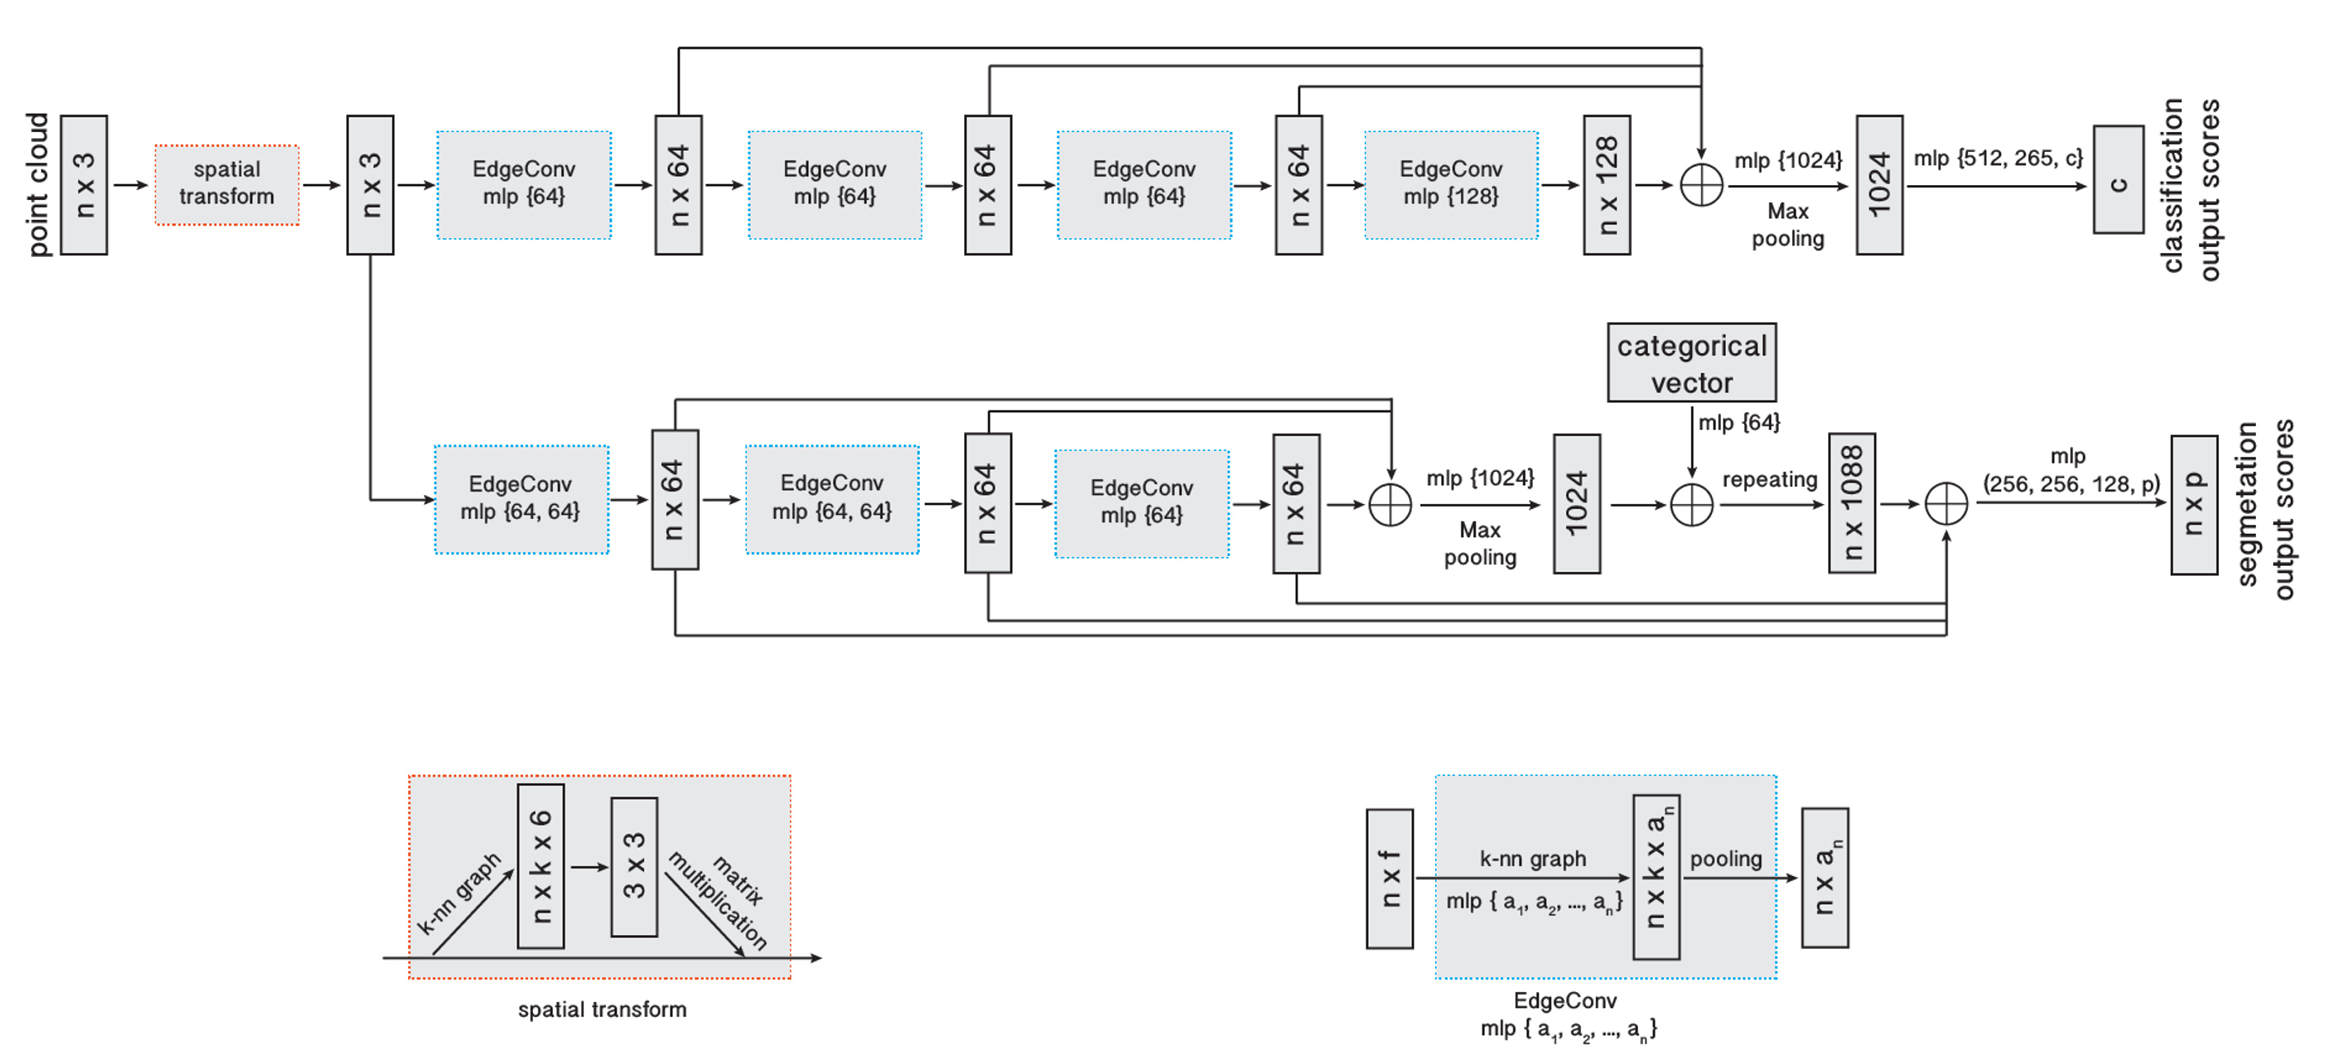
\includegraphics[width=430pt,height=300pt]{pictures/dgcnn_arch.jpg}
    \caption{The \ac{DGCNN} Architecture.\cite{wang2019dynamic}}
    \label{fig:dgcnn_arch}
\end{figure}

\vspace{5mm}

A directed graph $G = (V,E)$ which captures the topology of the point cloud where $V=\{p_i | i = \{1,2,...,n\}\}$ is the set of vertices and $E \subset V \times V$ is the set of edges. The graph $G$ is the \ac{k-NN} graph of $\mathcal{P}$ in $\mathbb{R}^F$. The graph has self-loops which means, each point in the point cloud has an edge to itself. The edge features computed by the EdgeConv block is defined as $e_{ij} = h_{\theta}(p_i, p_j)$ where $h_{\theta}: \mathbb{R}^F \times \mathbb{R}^F \rightarrow \mathbb{R}^{F'}$ is a non-linear function with a set of trainable parameters $\theta$. The EdgeConv operation is defined as a symmetric aggregation operation $\square$ which is applied on a channel wise manner. Summation or max are some of the examples of aggregation functions. It is applied on the edge features associated with all the edges that orginate from each connected vertex. Therefore, the output of the EdgeConv layer for $i$-th vertex is given by Eq. \ref{eq:EdgeConv}
\begin{equation}
    \label{eq:EdgeConv}
    p'_i = \underset{j:(i,j) \in E}{\square} h_{\theta}(p_i, p_j).
\end{equation}
Drawing similarity with convolution on images, $p_i$ is the central pixel and $\{p_j:(i,j) \in E\}$ is a patch around the central pixel as shown in Fig. \ref{fig:EdgeConv_op}. Therefore, for a point cloud with $F$ dimensions and $n$ points in it, the EdgeConv layer generates a point cloud with $F'$ dimensions and $n$ points in it.
\begin{figure}
    \centering
    \begin{minipage}[t]{.45\textwidth}
      \centering
      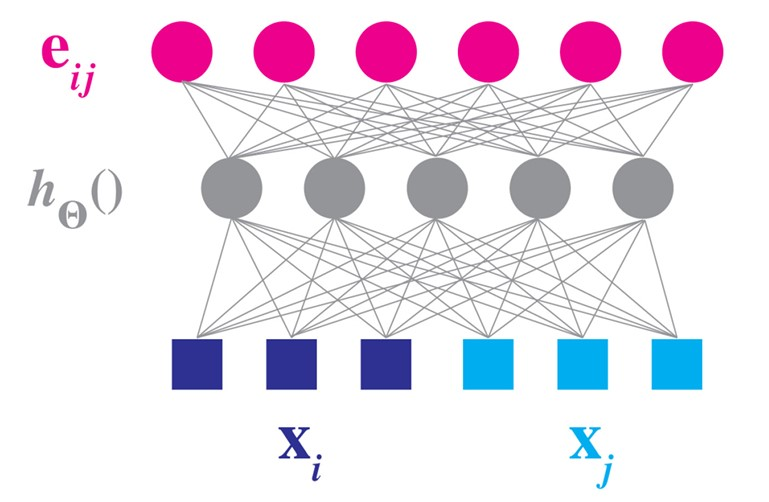
\includegraphics[width=200pt,height=120pt]{pictures/EdgeConv.jpg}
      \captionof{figure}{The Computation of edge feature $e_{ij}$ from a pair of points $p_i$ and $p_j$. Here, $h_{\theta}$ is a fully connected layer and the weights associated with it are the trainable parameters $\theta$.\cite{wang2019dynamic}}
      \label{fig:EdgeConv}
    \end{minipage}%
    \hspace{5mm}
    \begin{minipage}[t]{.45\textwidth}
      \centering
      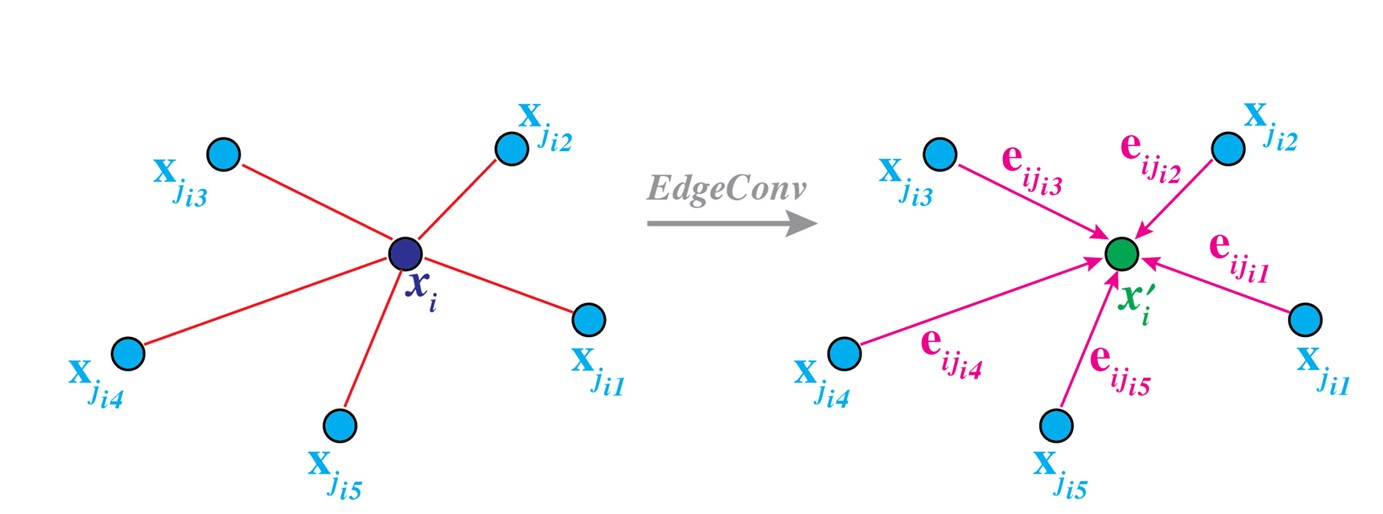
\includegraphics[width=200pt,height=150pt]{pictures/EdgeConv_op.jpg}
      \captionof{figure}{The EdgeConv operation. The output of EdgeConv is computed by aggregating the features associated with all the edges that orginate from each connected vertex.\cite{wang2019dynamic}}
      \label{fig:EdgeConv_op}
    \end{minipage}  
\end{figure}

\vspace{5mm}

Deciding the non-linear function $h_{\theta}$ and the symmetric aggregation function $\square$ plays a pivotal role in deciding the properties of the EdgeConv layer. To further illustrate on this point, if $p_1, ..., p_n$ are the points in the point cloud and the graph $G$ encapsulates the topological information of patches of fixed size around each central pixel, then if $\theta _m \cdot p_j$ is chosen as the non-linear function and sum is chosen as the aggregation operation, then it would behave as a standard convolution operation as in Eq. \ref{eq:std_conv}.
\begin{equation}
    \label{eq:std_conv}
    p'_{im} = \sum_{j:(i,j) \in E}\theta _m \cdot p_j,
\end{equation}
where $\theta = (\theta _1, \theta _2, ... , \theta _M)$ are the weights of $M$ different filters used in the convolution operation. Each entry in $\theta _m$ has the dimensionality as $p_i$ and $\cdot$ is the Euclidean inner product. Another variation of $h$ could be Eq. \ref{eq:EdgeConv_pointnet}. 
\begin{equation}
    \label{eq:EdgeConv_pointnet}
    h_{\theta}(p_i, p_j) = h_{\theta}(p_i).
\end{equation}
Here only the global embedding is taken into consideration and the non-linear function is unaware of the local features. This happens in PointNet and thus, it could be considered as a special case of EdgeConv. Another variation of $h$ as adapted by Atzmon \textit{et al.} in \cite{atzmon2018point} is Eq. \ref{eq:EdgeConv_gaussian} and Eq. \ref{eq:EdgeConv_gaussian_point}.
\begin{equation}
    \label{eq:EdgeConv_gaussian}
    h_{\theta}(p_i, p_j) = h_{\theta}(p_j).
\end{equation}
and 
\begin{equation}
    \label{eq:EdgeConv_gaussian_point}
    p'_{im} = \sum_{j \in V}(h_{\theta (p_j)})g(u(p_i,p_j)).
\end{equation}
Here $g$ is a Gaussian distribution kernel and $u$ calculates the pairwise Euclidean distance between the points in the point cloud. Another variation of $h$ could be to only capture the local features and ignore the global features based on the fact that the global shape is a collection of the local patches as shown in the following Eq. \ref{eq:EdgeConv_local}.
\begin{equation}
    \label{eq:EdgeConv_local}
    h_{\theta}(p_i, p_j) = h_{\theta}(p_j-p_i).
\end{equation}
The final variation of $h$ which is utilized by the authors in \cite{wang2019dynamic} is an asymmetric edge function as shown in Eq. \ref{eq:EdgeConv_asym}.
\begin{equation}
    \label{eq:EdgeConv_asym}
    h_{\theta}(p_i, p_j) = \bar{h_{\theta}}(p_i, p_j-p_i).
\end{equation}
This explicitly takes into account the global feature information as in Eq.\ref{eq:EdgeConv_pointnet} captured by the coordinates of the central pixel of the patch $p_i$ and the information of the local neighborhood as in Eq. \ref{eq:EdgeConv_local} and is captured by $p_j-p_i$. The EdgeConv operator is defined as 
\begin{equation}
    \label{eq:EdgeConv_op}
    e'_{ijm} = \ac{ReLU}(\theta _m \cdot (p_j - p_i) + \phi _m \cdot p_i).
\end{equation}
This operator could be implemented as a shared \ac{MLP} and then performing a max-pooling operation as in Eq. \ref{eq:EdgeConv_max}.
\begin{equation}
    \label{eq:EdgeConv_max}
    p'_{im} = \underset{j:(i,j) \in E}{max}e'_{ijm},
\end{equation}
where $\theta = (\theta _1, \theta _2, ... , \theta _M)$ are the weights of $M$ different filters used in the convolution operation.

\vspace{5mm}

\textbf{Dynamic Graph Update} A crucial point in this network is to regenerate the graph using \ac{k-NN} in the feature space after each layer. This is the main difference of this network as compared to traditional graph \ac{CNN} for which there is a fixed graph for all the layers of the network. Because the graph is updated after every layer, the architecture gets its name the \ac{DGCNN}. With dynamically updating the graph after each layer, the receptive field increases to as large as diameter of the point cloud, even if the points in the point cloud are sparse. Thus, after each layer a different graph is computed $G^{(l)} = (V^{(l)}, E^{(l)})$, where $G^{(l)}$ is a graph in the $l$-th layer with vertices $V^{(l)}$ and edges $E^{(l)}$ which can be denoted as $(i,j_{i1}), ... , (i,j_{ik_{l}})$ such that $p_{j_{i1}}^{(l)}, ... , p_{j_{ik_{l}}}^{(l)}$ are the k-nearest points closest to point $p_i$ at layer $l$. In other words, the model constructs a different graph for each point in the point cloud after every layer where the nearest points and the edges emerging from a vertex(point in the point cloud in the case) changes at every layer. A pairwise distance matrix in the feature space is used to calculate the k-nearest points of each point in the point cloud. As a result of this, the network has the following properties,
\begin{itemize}
    \item \textit{Invariant to permutations}. The output of an EdgeConv layer is given by
    \begin{equation}
        \label{eq:EdgeConv_perm}
        p'_{i} = \underset{j:(i,j) \in E}{max}h_{\theta}(p_i,p_j). 
    \end{equation}
    Because of the usage of a max operator which is symmetric in nature, the output of the layer $p'_{i}$ is permutation invariant to the order in which $p_i$ appears in the input point cloud. Other functions which are symmetric (eg. $\sum$) in nature can also be applied here instead of max. The global max pooling operator used to aggregate point features is a symmetric function and thus, gives permutation invariant results.
    \item \textit{Invariant to translation.} The EdgeConv operator satisfies "partial" translation invariance. If a translation $T$ is applied to the points $p_i$ and $p_j$ of the point cloud $\mathcal{P}$, then applying translation to Eq. \ref{eq:EdgeConv_op}, the translated point cloud would be 
    \begin{equation}
        \label{eq:EdgeConv_trans}
        \begin{split}
            e'_{ijm} &= \theta _m \cdot (p_j + T - (p_i + T)) + \phi _m \cdot (p_i + T),\\
            &= \theta _m \cdot (p_j - p_i) + \phi _m \cdot (p_i + T).
        \end{split}    
    \end{equation}
    Therefore, if $\phi _m =0$, then EdgeConv operator is completely translation invariant. But this however restricts the model to recognize an object depending on only the unordered set of patches, i.e. it disregards the orientation and the exact location of the patches. On the other hand, with both $p_j-p_i$ and $p_i$, the model considers both the local orientation of the patches as well as the global information about the shape of the object. 
\end{itemize}

\subsubsection{Point-level Clustering Module}
\begin{figure}[t]
    \centering
    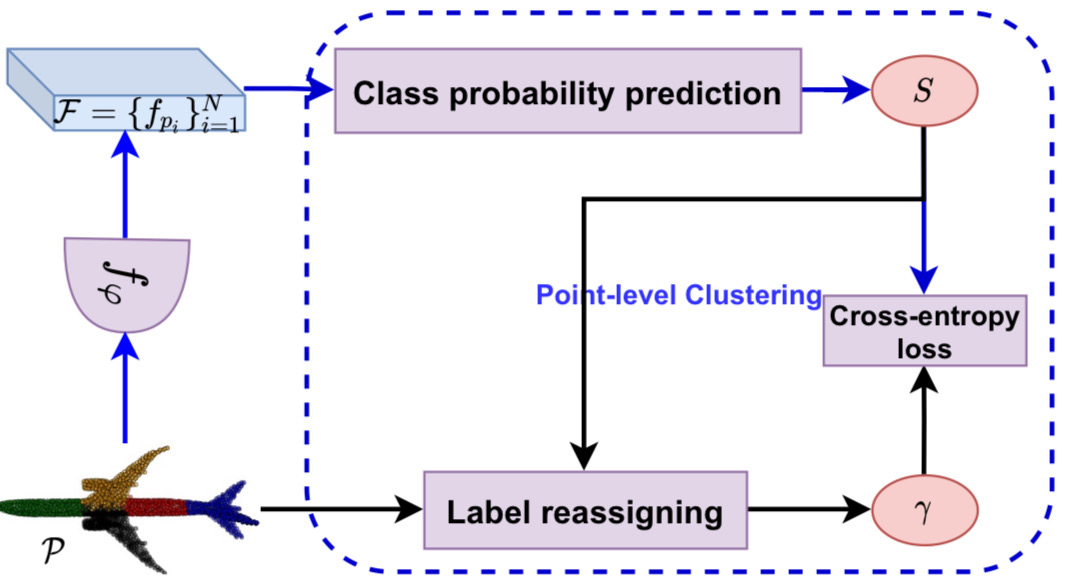
\includegraphics[width=300pt,height=180pt]{pictures/point_level.jpg}
    \caption{The architecture of the point-level clustering based unsupervised feature learning.\cite{mei2022unsupervised}}
    \label{fig:point_level}
\end{figure} 
 Now, the model already has the feature representation from the feature encoder backbone (eg. PointNet or  \ac{DGCNN}). The next step is the point-level clustering module. Fig.\ref{fig:point_level} gives a detailed visualization of the point-level clustering module. It can be seen that it is made up of 2 entities, the "class probability prediction" function and the "label reassigning". The point-level clustering module is analogous to the semantic segmentation task. Each point $p_i$ of the point cloud $\mathcal{P}$ is assigned to one of the $J$ predetermined possible subgroups or semantic categories. Essentially, it is achieved by processing each of the point cloud $\mathcal{\textbf{P}}$ followed by a point-level class probability prediction operator that yields a matrix for class probability $\mathit{\textbf{S}} = \{ s_{ij} \in [0,1]\}_{i,j}^{N,J}$. The label reassigning operator thus, takes the point cloud $\mathcal{\textbf{P}}$ and the class probability matrix $S$ and generates a pseudo-label matrix $\mathit{\mathbf{\gamma}} = \{ \gamma_{ij} \in \{0,1\}\}_{i,j}^{N,J}$. The weights for the encoder $f_{\varphi}$ are learnt such that it minimizes the average cross-entropy loss between the pseudo-label $\gamma$ and the predicted class probability $\textbf{S}$. The average cross entropy loss is calculated by the formula given in Eq.\ref{eq:avg_cross_entropy}.
\begin{equation}
    \label{eq:avg_cross_entropy}
    \mathit{H}(\gamma,\textbf{S})= \mathit{ - \frac{1}{N}} \langle \gamma,\log \textbf{S} \rangle = \mathit{ - \frac{1}{N}} \sum_{i=1}^{N} \sum_{j=1}^{J} \gamma_{ij} \log s_{ij}.
\end{equation}
But to train a network with a cross-entropy loss, the ground truth labels of the points in the point cloud are required. Since that is not available, one needs to assign the label $\gamma$ automatically, which is explained in details in the following passage. 

\subsubsection*{Class Probability Prediction}
As mentioned in the last passage, the output of the encoder $f_{\varphi}$ is fed as input to a classification head $\phi_\alpha$ and it generates a logit score for each of the feature vector as shown in Fig.\ref{fig:class_prob}. The vector for the logit score is given by $\textbf{g}_i = (g_{i1}, g_{i2},....., g_{iJ}), where \textbf{g}_i = \gamma_\alpha(f_{p_i})$. The classification head has 2 fully connected layers where each layer is a linear layer followed by a batch normalization. The leakyReLU activation function is used in all the layers except the last layer. As the output of the last layer N vectors for each of the N points in the point cloud is received where each of the output vector has $J$ dimensions, the number of predetermined subcategories each point cloud is to be segmented into. Thus, each entry of the feature vector is the probability of that point belonging to $j$-th category. Therefore, the logit score matrix $\textbf{G} = \{ g_{ij}\}_{i,j}^{N,J}$ has the dimension $N \times J$. The prediction that the point $p_i$ belongs to the category $j$ is computed by the application of a row-wise softmax operation on $\textbf{G}$ given by Eq.\ref{eq:softmax}.
\begin{equation}
    \label{eq:softmax}
    \mathit{s_{ij}}= \mathit{\frac{exp(g_{ij})}{\sum_{l=1}^{J}exp(g_{ij})}}. 
\end{equation}

\begin{figure}
    \centering
    \begin{minipage}[t]{.45\textwidth}
      \centering
      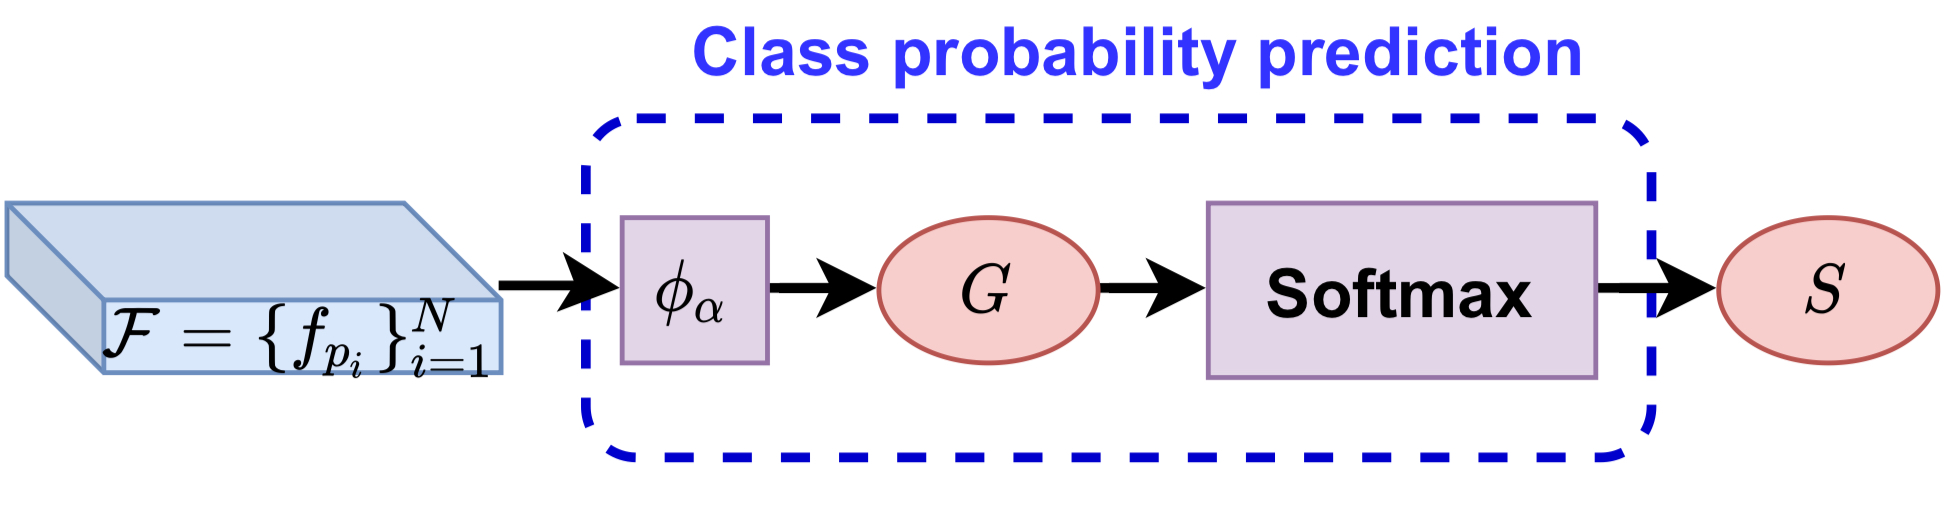
\includegraphics[width=200pt,height=100pt]{pictures/class_prob.jpg}
      \captionof{figure}{Architecture of class probability prediction.\cite{mei2022unsupervised}}
      \label{fig:class_prob}
    \end{minipage}%
    \hspace{1cm}
    \begin{minipage}[t]{.45\textwidth}
      \centering
      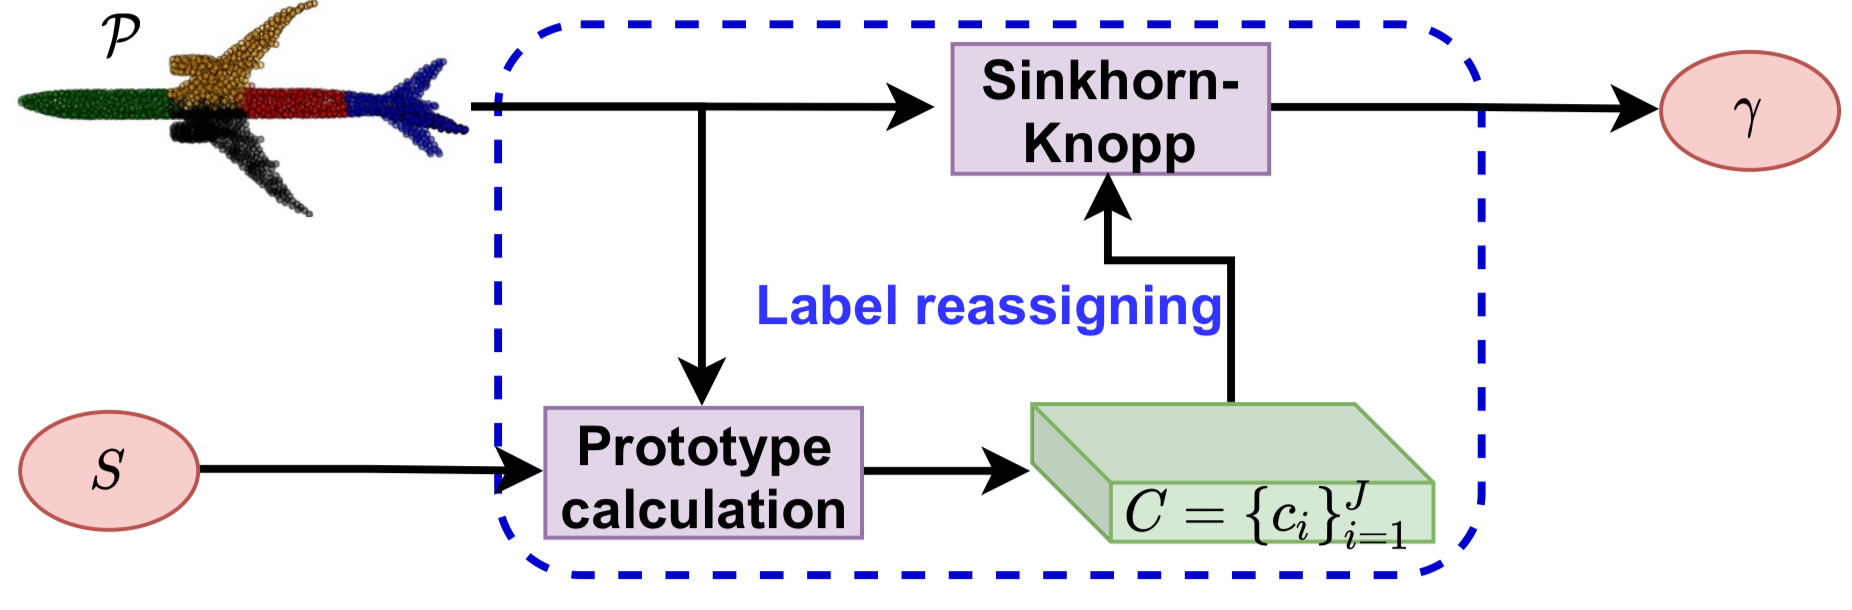
\includegraphics[width=200pt,height=100pt]{pictures/label_reassign.jpg}
      \captionof{figure}{Architecture of label reassigning \cite{mei2022unsupervised}}
      \label{fig:label_reassign}
    \end{minipage}
\end{figure}

\subsubsection*{Label reassigning}
In order to calculate the labels shown in Fig.\ref{fig:label_reassign}, the representative members of each of the semantic subgroups is needed. It can be done by selecting the cluster mean or cluster centers of each of these subgroups as the representative member of the cluster. The class probability matrix $S$ can be infered as the soft assignment of each point $p_i$ in the point cloud to $J$ semantic partitions. So the softly weighted mean of each of these partitions can be calculated as in Eq.\ref{eq:soft_mean}.

\begin{equation}
    \label{eq:soft_mean}
    \mathit{c_{j}}= \mathit{\frac{1}{\sum_{i=1}^{N}s_{ij}}\sum_{i=1}^{N}s_{ij}\mathbf{p}_i, j = 1,2,....,J}, 
\end{equation}
or in another way $C= \{c_j\}_{j_1}^J$ is a matrix with dimensions $J \times 3$. In a completely unsupervised learning setup, $\gamma \in [0,1]$ can be visualized as the posterior probability of a $p_i$ belong to the $j-th$ partition. $\gamma$ is optimized in the same method as in Eq.\ref{eq:softmax}. This results in a degenerate solution where each point is assigned to a single category. Thus, two assumptions are very pivotal for the reassigning of the labels. Firstly, the points in the point cloud ought to be partitioned into "equally-sized" partitions. In other words it can be formulated as $\mathit{\sum_{i=1}^{N}\gamma_{ij} = \frac{N}{J}}$. This is extremely importance in order to pretend all the points in the point cloud to be assigned to a single partition. Secondly, since the idea of using cluster centers as representative members of the partitions is inspired from the k-means algorithm, it means that if a point $p_i$ of the point cloud belongs to the $j^{*}$-th partition, the distance from $p_i$ to $c_j$ should be the shortest as compared to the distance of $p_i$ to all other cluster centers. In other words $ \lVert \mathbf{p}_i - c_{j^*} \rVert _2 \leq \lVert \mathbf{p}_i - c_{j} \rVert _2, j \neq j^* $. This is also equivalent to $ min_{\gamma}\sum_{i=1}^{N}\sum_{j=1}^{J} \gamma_{ij} \lVert \mathbf{p}_i - c_{j} \rVert _2^2$. This objective function is optimized to get $\gamma$. As per the rules of probability, the sum of all possible outcomes of an event is equal to 1, therefore $\sum_{j=1}^{J} \gamma_{ij} = 1$. Thus, the matrix of joint probability can be formulated as $\Gamma$ as $\Gamma = \frac{\gamma}{N}$ which has the elements $\Gamma_{ij} = \frac{\gamma_{ij}}{N}$. The distance matrix $\mathit{D = \{d_{ij}\}_{i,j}^{N,J}}$ has dimensions $\mathit{N \times J}$ where each element $\mathit{d_{ij}}$ is defined as $\mathit{d_{ij}} = \lVert \mathbf{p}_i - c_{j} \rVert _2^2$. In accordance to the assumptions stated above, the objective function $\mathit{D}$ could be minimized with respect to $\Gamma$ as in Eq.\ref{eq:label_reassign}.
\begin{equation}
    \label{eq:label_reassign}
    \begin{split}
        &\underset{\Gamma}{min \langle \Gamma, D \rangle},\\
        &s.t., \Gamma^{T}\vec{1}_{\mathit{N}} = \frac{1}{\mathit{J}}\vec{1}_{J} =, \Gamma\vec{1}_{J} = \frac{1}{\mathit{N}}\vec{1}_{\mathit{N}},
    \end{split}    
\end{equation}
where $\vec{1}_{J}$ is the vector of ones having dimension $J$. The above condition enforces that each of the cluster representative is  selected atleast $\frac{N}{J}$ times for each point cloud and $\sum_{j=1}^{J}\gamma_{ij}=1$. The objective function as defined in Eq.\ref{eq:label_reassign} is a typical case of an optimal transport problem \cite{peyre2019computational}. Such problems can be solved by the Sinkhorn-Knopp algorithm \cite{cuturi2013sinkhorn}. In other words, it means solving the entropic regularized objective function in Eq. \ref{eq:entropy_regular}.
\begin{equation}
    \label{eq:entropy_regular}
    \begin{split}
        &\underset{\Gamma}{min \langle \Gamma, D \rangle} - \lambda \mathit{H}(\Gamma),\\
        &s.t., \Gamma^{T}\vec{1}_{\mathit{N}} = \frac{1}{\mathit{J}}\vec{1}_{J} =, \Gamma\vec{1}_{J} = \frac{1}{\mathit{N}}\vec{1}_{\mathit{N}},
    \end{split}    
\end{equation}
where, $\mathit{H}(\Gamma) = \langle \Gamma, \log \Gamma -1 \rangle $ is the entropy of $\Gamma$ and $\lambda$ is the regularization parameter. As per \cite{cuturi2013sinkhorn}, on solving Eq. \ref{eq:entropy_regular}, the normalized exponential matrix in Eq. \ref{eq:gamma} is attained. 
\begin{equation}
    \label{eq:gamma}
    \Gamma = diag(\mu) exp(\mathit{D/\lambda}) diag(\nu),
\end{equation}
where $\mu$ and $\nu$ are renormalized vectors in $\mathbb{R}^N$ and $\mathbb{R}^J$ respectively and $exp()$ is the exponential function. These vectors are computed on utilizing the iterative Sinkhorn-Knopp algorithm\cite{cuturi2013sinkhorn} with the constraints $ \mu = \frac{1}{\mathit{N}} \vec{1}_{\mathit{N}} $ and $ \nu = \frac{1}{\mathit{J}} \vec{1}_{\mathit{J}} $. The pseudo-code for the Sinkhorn-Knopp algorithm is elaborated in Algorithm \ref{alg:sinkhorn}.

\begin{algorithm}[h]
    \caption{Pseudo-code for Sinkhorn-Knopp algorithm}\label{alg:sinkhorn}
    def sinkhorn($D, \epsilon, niters=3$)
    \begin{algorithmic}[1]
        \State $\Gamma = exp(D/ \epsilon)^T$
        \State $\gamma /= sum(\Gamma)$
        \State $N, J = \Gamma .shape$
        \State $u,r,c = zeros(N), ones(J)/J, ones(N)/N$
        \For{$\; in range (0, \; niters)$}
            \State $u = sum(\Gamma, dim=1)$
            \State $\Gamma *= (r/u).unsqueeze(1)$
            \State $\Gamma *= (c/sum(\Gamma, dim=0)).unsqueeze(0)$            
        \EndFor
        \State $\mathbf{return} \; \Gamma$          
    \end{algorithmic}
\end{algorithm}

Thus, the overall point-level clustering can be encapsulated by an \ac{EM} like algorithm. The network learns the parameters $f_{\varphi}$ and $\mathcal{\phi}_{\alpha}$ by optimization of Eq.\ref{eq:avg_cross_entropy} and get a label reassigning matrix $\gamma$ by solving the optimization problem in Eq. \ref{eq:gamma} with respect to $\Gamma$. It is executed by performing the following steps in repetition. 
\begin{itemize}
    \item Step 1: representation learning. Having the current probability matrix $\gamma$, the weights of the model are updated by optimizing Eq. \ref{eq:avg_cross_entropy} with respect to the  parameters $f_{\varphi}$ and $\mathcal{\phi}_{\alpha}$. It is in line with the supervised case where the model uses the cross entropy loss for classification. 
    \item Step 2: label reassigning. On having the updated set of $f_{\varphi}$ and $\mathcal{\phi}_{\alpha}$, $\Gamma$ is calculated by using Eq. \ref{eq:gamma}. The posterior probability matrix is then computed by $\gamma = \mathit{N} \cdot \Gamma$.
\end{itemize}
Thus, each update step requires a single matrix-vector multiplication which has the time complexity of $O(\mathit{N \times J})$ which means the computation time increases linearly with the increase in the number of points in the point cloud. Therefore, scalability of this method is quite high and the process remains relatively quick even for a million samples in the dataset. Moreover, the orthogonal regularization is introduced to circumvent the issue of having the same output vector for all cluster representatives. It is computed by 
\begin{equation}
    \label{eq:orth}
    \mathcal{L}_{\mathit{orth}}(\mathit{C}) = \lVert \mathit{C_{*}^{T} C_{*} - I} \rVert _{1},
\end{equation}
where $ \lVert \cdot \rVert _1 $ is the $l_{1}$-norm or the Manhattan distance and $\mathit{C_{*}} = [ \frac{c_1}{\lVert c_1 \rVert _{2}}, \frac{c_2}{\lVert c_2 \rVert _{2}}, ... , \frac{c_{\mathit{J}}}{\lVert c_{\mathit{J}} \rVert _{2}}]$. The pseudo-code for the point-level clustering module in elaborated in Alg. \ref{alg:point_level}.

\begin{algorithm}[H]
    \caption{Pseudo-code for point-level clustering}\label{alg:point_level}
    \textbf{Input:} $\{\mathcal{P}\}$: is a set of 3D point clouds with $\mathit{N}$ number of points in it; $\mathit{K}$: number of epochs. \\
    \textbf{Output:} backbone $f_{\varphi}$.
    \begin{algorithmic}[1]
        \For{$i$ in range $(0,K)$}
            \State $\mathcal{L} = 0$
            \For{$\mathcal{P} \in \{\mathcal{P}\}$}
                \State \# Computes Class probability
                \State $ S = softmax(\phi_{\alpha}(f_{\varphi}(\mathcal{P})))$
                \State \# Computes cluster representatives of partitions
                \State $ C = \left\{ \frac{1}{\sum_{i=1}^{N}s_{ij}} \sum_{i=1}^{N}s_{ij}\mathbf{p}_i \right\}_{j=1}^N$
                \State \# Computes mean-squared error 
                \State $ D = \left\{ \lVert \mathbf{p}_i - c_j \rVert _2^2 \right\} _{i,j}^{N,J}$
                \State \# Computes posterior probability matrix
                \State $\gamma = sinkhorn(\ac{stop-grad}(D), 1e - 3, 20)$
                \State \# Computes Loss Function 
                \State $\mathcal{L} = H(\gamma,S) + \eta \mathcal{L}_{orth}(C)$
            \EndFor
            \State \# Updates backbone, projector ad predictor
            \State $ f_{\varphi}, \phi_{\alpha} \gets optimize(\frac{\mathcal{L}}{N})$
        \EndFor
        \State $\mathbf{return \; f_{\varphi}}$          
    \end{algorithmic}
\end{algorithm}

\subsubsection{Instance-Level Contrasting Module}
\begin{figure}[t]
    \centering
    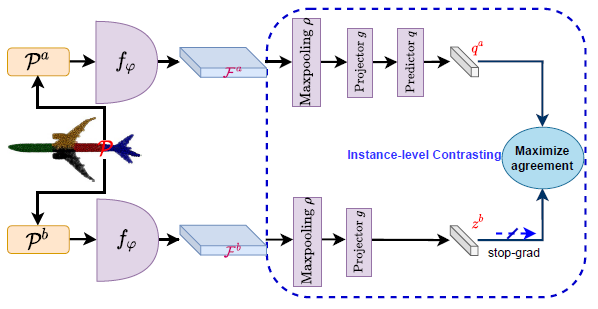
\includegraphics[width=300pt,height=180pt]{pictures/ConClu.png}
    \caption{The architecture of the instance-level Contrasting.\cite{mei2022unsupervised}}
    \label{fig:global_level}
\end{figure} 
This module plays a crucial role in learning the global features of the point clouds. The architecture of this module is shown in Fig. \ref{fig:global_level}. The network is fed with two augmented views $\mathcal{P}^a$, $\mathcal{P}^b$ of the same point cloud $\mathcal{P}$. The feature representation obtained as the output of the encoder backbone $f_{\varphi}$, are fed to a MaxPooling layer $\rho$, the output of which is fed to a projection \ac{MLP} head $g$ \cite{chen2021exploring}. The encoder backbone $f_{\varphi}$ and the projection head $g$ shares the weights for both the augmented views. The output of the projection head of one of the augmented views (the top branch) is fed to the prediction head $q$. The purpose of this unit is to transform the output of one of the augmented views to match the other. The operation is applied to only one augmented view to make the network asymmetric \cite{grill2020bootstrap}. In other words, the output vectors can be realized as  $ \mathit{q^a} \triangleq \mathit{\mathbf{q}(g(\rho(\mathbf{\mathcal{F}}^a)))}$ and $\mathit{\mathbf{z}^b} \triangleq \mathit{g(\rho(\mathbf{\mathcal{F}}^b))}$ where $\mathbf{\mathcal{F}}^a = f_{\phi}(\mathbf{\mathcal{P}}^a)$ and $\mathbf{\mathcal{F}}^b = f_{\phi}(\mathbf{\mathcal{P}}^b)$. Keeping in line with \cite{chen2021exploring}, \ac{stop-grad} is applied on the second branch $z^b$ to resist the network from generating a constant mapping without using negative samples for contrastive learning. The network is constructed such that the similarity between $\mathit{q^a}$ and $\mathit{z^b}$ is maximized. Mathematically speaking, the mean-squared error between the $\mathit{l}_2$-normalized prediction $q^a$ and projection $\mathit{z_b}$ is minimized as shown in Eq. \ref{eq:error}. 
\begin{equation}
    \label{eq:error}
    \mathcal{D}(\mathit{q^a, z^b}) \triangleq \lVert \frac{\mathit{q^a}}{\lVert \mathit{q^a} \rVert _2} - \frac{\mathit{z^b}}{\lVert \mathit{z^b} \rVert _2} \rVert _2^2 = 2 - \frac{2\mathit{q^{aT}z^b}}{\lVert q^a \rVert _2 \cdot \lVert z^b \rVert _2}.
\end{equation}

In other words, it is the negative cosine similarity, up to a scale of 2. Since, \ac{stop-grad} is enforced on $z^b$, Eq. \ref{eq:error} is modified by the following Eq. \ref{eq:error_stop-grad}.
\begin{equation}
    \label{eq:error_stop-grad}
    \mathcal{D}(\mathit{q^a, \ac{stop-grad}(z^b)}), 
\end{equation}
which means $z^b$ acts as a constant vector in this equation. Keeping in line with \cite{chen2021exploring}, a global symmetrized loss is defined as in Eq. \ref{eq:sym_loss}.
\begin{equation}
    \label{eq:sym_loss}
    \mathcal{L}_{\mathit{global}} = \mathcal{D}(\mathit{q^a, \ac{stop-grad}(z^b)})  + \mathcal{D}(\mathit{q^b, \ac{stop-grad}(z^a)}). 
\end{equation}
The minimum value the above equation can attain is 0. This is because, in the first term of the equation, the encoder backbone $q^a$ gets no gradient flow from $z^b$. But it gets gradients from $q^b$ in the second term. In the same way, in the second term of the equation, the encoder backbone $q^b$ gets no gradient flow from $z^a$. But it gets gradients from $q^a$ in the first term. if the \ac{stop-grad} mechanism is not applied, then in spite of having a loss of zero during training, the representations learnt by the network would be futile i.e. all the point clouds would be mapped to the same feature representation. Or in other words, the network would crumble to  constant mapping \cite{chen2021exploring}. The pseudo-code for this module is shown in Alg. \ref{alg:instance_level}.

\begin{algorithm}[H]
    \caption{Pseudo-code for instance-level clustering}\label{alg:instance_level}
    \textbf{Input:} $\{\mathcal{P}\}$: is a set of 3D point clouds with $\mathit{N}$ number of points in it; $\mathit{K}$: number of epochs. \\
    \textbf{Output:} backbone $f_{\varphi}$.
    \begin{algorithmic}[1]
        \For{$i$ in range $(0,K)$}
            \State $\mathcal{L} = 0$
            \For{$\mathcal{P} \in \{\mathcal{P}\}$}
                \State \# Generate random augmentations
                \State $ \mathcal{P}^a = aug(\mathcal{P})$
                \State $ \mathcal{P}^b = aug(\mathcal{P})$
                \State \# Compute projections
                \State $\mathit{z^a = g(\rho(f_{\varphi}(\mathcal{P}^a)))}$
                \State $\mathit{z^b = g(\rho(f_{\varphi}(\mathcal{P}^b)))}$
                \State \# Compute predictions
                \State $\mathit{q^a, q^b = q(z^a), q(z^b)}$
                \State \# Calculate loss
                \State $\mathcal{L} += \mathcal{D}(\mathit{q^a, \ac{stop-grad}(z^b)})  + \mathcal{D}(\mathit{q^b, \ac{stop-grad}(z^a)})$
            \EndFor
            \State \# Updates backbone, projector ad predictor
            \State $ f_{\varphi}, g, q \gets optimize(\frac{\mathcal{L}}{N})$
        \EndFor
        \State $\mathbf{return \; f_{\varphi}}$          
    \end{algorithmic}
\end{algorithm}

\subsubsection{Loss Function}
The objective of the network is to simultaneously minimize both the point-level clustering loss and the instance level contrasting loss. If the two augmented views of the point cloud $\mathcal{P}$ are $\mathcal{P}^a$ and $\mathcal{P}^b$, then the point-level clustering loss can be calculated by Eq. \ref{eq:local_loss}.
\begin{equation}
    \label{eq:local_loss}
    \mathcal{L}_{\mathit{local}} = H(\gamma^{a}, S^a) + H(\gamma^{b}, S^b) + \eta(\mathcal{L}_{orth}(C^a) + \mathcal{L}_{orth}(C^b))
\end{equation}
where $\eta>0$ is a regularization parameter. Here $\gamma^a$ is the posterior class probability of the point belonging to one of the subcategories, $S^a$ is the predicted class probability and $C^a$ is the normalized center of the augmented view of the point cloud $\mathcal{P}^a$. In the same way, the corresponding terms for the other augmented view $\mathcal{P}^b$ are $\gamma^b$, $S^b$ and $C^b$. Therefore, the total loss could be calculated as the linear combination of $\mathcal{L}^{global}$ and $\mathcal{L}^{local}$ as in Eq. \ref{eq:total_loss}.
\begin{equation}
    \label{eq:total_loss}
    \mathcal{L}_{\mathit{total}} = \mathcal{L}_{\mathit{local}} + \mathcal{L}_{\mathit{global}}.
\end{equation}

\subsection{Dimensionality Reduction}
\subsubsection{Reasons for Dimension Reduction}
The goal of this thesis is to find a diverse set of objects that collectively represent the entire ABC dataset \cite{Koch_2019_CVPR}. This set of objects is to be then used as the source library for the different transfer learning approaches to be used in bin picking applications. Therefore, clustering algorithms are necessary to find the representative members of the dataset. In order to facilitate the usage of the \ac{DBCV} Index as the evaluation metric for the clustering algorithm as mentioned in Ch. \ref{sec:dbcv}, it is necessary to reduce the dimensions of the latent space representations. Furthermore, it would be beneficial to find lesser but denser clusters. This means that fewer objects could collectively represent the entire dataset and each representative member would be similar to a greater number of other objects in the dataset. Thus, reducing the dimensions of the latent space representations by dimensionality reduction would entail more "crowded" clusters in case of density-based clustering algorithms.

\subsubsection{T-distributed Stochastic Neighbor Embedding}
A technique for reducing dimensionality, \ac{t-SNE} is mostly used for data visualization in 2D and 3D maps. This approach has become well-liked since it can identify non-linear relationships in the data. If the data has more than two or three features, it might be necessary to consider looking for clusters in the data. To better understand the data and determine how many clusters to use in clustering models like k-means, if necessary. To further grasp what one hopes to obtain, the following example is used for illustration. It is assumed that the data is to be converted from a 2D space to a 1D dimension as shown in Fig. \ref{fig:2d_data} and Fig. \ref{fig:1d_data} respectively.\cite{van2008visualizing}

\begin{figure}
    \centering
    \begin{minipage}[t]{.45\textwidth}
      \centering
      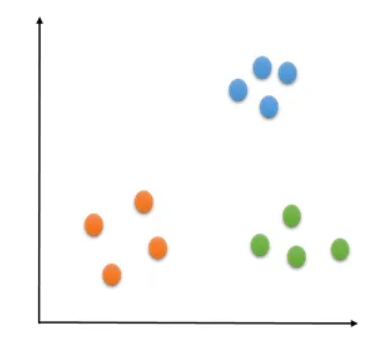
\includegraphics[width=150pt,height=120pt]{pictures/2d_data.PNG}
      \captionof{figure}{The original data in 2-D space \cite{tsne}.}
      \label{fig:2d_data}
    \end{minipage}%
    \hspace{5mm}
    \begin{minipage}[t]{.45\textwidth}
      \centering
      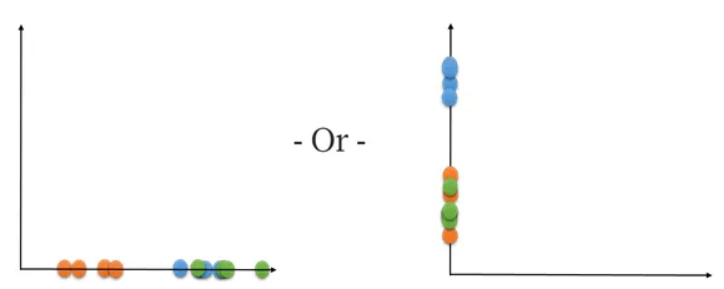
\includegraphics[width=200pt,height=120pt]{pictures/1d_data.PNG}
      \captionof{figure}{Data projected to 1-D space \cite{tsne}.}
      \label{fig:1d_data}
    \end{minipage}  
\end{figure}
Every color in this illustration denotes a cluster. It is evident that the densities of each cluster differ. It can be observed that at least two of the clusters overlap when a simple projection of the data onto one of its dimensions is performed. This highlights that a better method is necessary for the dimension reduction task. This problem is handled by the \ac{t-SNE} algorithm and its effectiveness is described in the following steps.
\begin{itemize}
    \item Determining a joint probability distribution that captures the commonalities amongst the data points.\cite{van2008visualizing}
    \item Constructing a dataset of the points with the target dimension and thereafter computing the joint probability distribution of those points as well.\cite{van2008visualizing}
    \item Gradient descent is used to transform the low-dimensional dataset into a joint probability distribution that is as close as feasible to the high-dimensional dataset.\cite{van2008visualizing}
\end{itemize}

\vspace{5mm}

\textbf{Working principle of \ac{t-SNE}}\\
\begin{enumerate}
    \item \textbf{The likelihood of points to belong to the same neighborhood}\\
    Finding each point's Euclidean distance from every other point is the initial step in the process. Next, these distances are converted into conditional probabilities, which express how similar one pair of points is to the other. This means that it is required to determine the degree of similarity—that is the likelihood—between any two points in the data. A Gaussian distribution with a standard deviation of $\sigma_i$ and a center at $x_i$ represents the conditional probability of point $x_j$ to be next to point $x_i$. The conditional probability is defined mathematically as shown in Eq. \ref{eq:cond_prob}. The factors that effect $\sigma_i$ are discussed later.
    \begin{equation}
        \label{eq:cond_prob}
        \mathit{p_{j|i}} = \mathit{\frac{exp \left(- \frac{\lVert x_i - x_j \rVert ^2}{2 \sigma_i^2} \right)}{\sum_{k \neq i} exp \left(- \frac{\lVert x_i - x_k \rVert ^2}{2 \sigma_i^2} \right)}}, 
    \end{equation}
    where $p_{j|i}$ is the probability that the point $x_i$ has $x_j$ as its neighbor. Since the clusters can have varying densities, the division by the total of all the other points positioned at the Gaussian distribution centered at $x_i$ is necessary. Looking back to Fig. \ref{fig:2d_data} as an example to clarify, the orange cluster has a lesser density than the blue. As a result, there will be less similarity between the orange and blue points if the Gaussian distribution is used to compute the commonalities between each pair of points. The normalization is performed because it is only necessary to view the clusters as such in the final output and if any of the clusters have differing densities need not be visualized. The joint probability distribution can be computed from the conditional distributions as shown in Eq. \ref{eq:joint_prob}.\cite{van2008visualizing}
    \begin{equation}
        \label{eq:joint_prob}
        \mathit{p_{ij}} = \mathit{\frac{p_{j|i} + p_{i|j}}{2n}}. 
    \end{equation}
    One of the ways that the t-SNE approach differs from the previous SNE is that it uses the joint probability distribution instead of the conditional probability. The computation in the third stage of the algorithm is made simpler by the symmetric property of the pairwise similarities $(p_{ij} = p_{ji})$.
    \item \textbf{Transformation of the data to a lower dimension}\\
    In this step, a joint probability distribution for the points in the low-dimensional space is computed. In order to achieve that, a new dataset is created at random that has K features (K being the desired dimension) and the same amount of points as the original dataset. As the dimension reduction is performed for visualization, K will often be two or three. Returning to the example, the \ac{t-SNE} algorithm now creates a random dataset of 1D points as shown in Fig. \ref{fig:random_1d_data}.
    \begin{figure}
        \centering
        \begin{minipage}[t]{.45\textwidth}
          \centering
          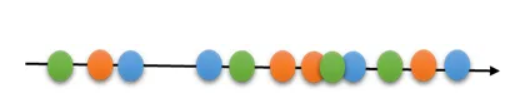
\includegraphics[width=150pt,height=50pt]{pictures/random_1d_data.PNG}
          \captionof{figure}{A random dataset created in 1D space \cite{tsne}.}
          \label{fig:random_1d_data}
        \end{minipage}%
        \hspace{5mm}
        \begin{minipage}[t]{.45\textwidth}
          \centering
          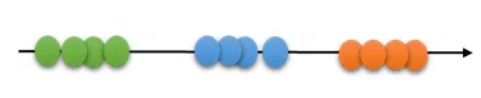
\includegraphics[width=150pt,height=50pt]{pictures/tsne_output.PNG}
          \captionof{figure}{Visualization of the dataset in 1D space after applying \ac{t-SNE} \cite{tsne}.}
          \label{fig:tsne_output}
        \end{minipage}  
    \end{figure}
    Similar to the original dataset, the joint probability distribution for this set of points is generated using the t-distribution rather than the Gaussian distribution. The points in this case are denoted as $y$ and the probabilities as $q$ and thus, the joint probability distribution is computed as shown in Eq. \ref{eq:joint_prob_random}.
    \begin{equation}
        \label{eq:joint_prob_random}
        \mathit{q_{ij}} = \frac{\left(1 + \lVert y_i - y_j \rVert\right) ^{-1}}{\sum_{k \neq l}\left(1 + \lVert y_k - y_l \rVert\right) ^{-1}}.
    \end{equation}
    The heavy tails attribute of the t-distribution is the rationale behind selecting it over the Gaussian distribution. This property helps minimize "crowding" of the points in the lower dimension by making moderate gaps between points in the high-dimensional space. An additional benefit of employing the t-distribution is that it enhances the algorithm's optimization procedure in the third stage.\cite{van2008visualizing}
    \item \textbf{Modification of the dataset in the low-dimensional space for the best possible data visualization}\\
    Now, the \ac{KL} divergence is utilized to maximize the similarity between the joint probability distribution of the data points in the low dimensional space and the higher dimensional space. The \ac{KL} divergence serves as a gauge for the degree of difference between two distributions. It is defined for distributions P and Q in the probability space of $\chi$ by Eq. \ref{eq:kl_div}.
    \begin{equation}
        \label{eq:kl_div}
        \mathit{D}_{\ac{KL}}(\mathit{P} || \mathit{Q}) = \sum_{x \in \chi} \mathit{P(x)} \log \left( \frac{\mathit{P(x)}}{\mathit{Q(x)}} \right).
    \end{equation}
    In instances where the distributions are identical, the KL divergence value approaches to 0, indicating an increase in similarity between the distributions. The lower dimension dataset is modified so that, in the joint probability distribution, it resembles the original data as soon as possible. To do this, gradient descent is used. The KL divergence between the joint probability distributions P from the high-dimensional space and Q from the low-dimensional space is the cost function that the gradient descent algorithm seeks to minimize as defined in Eq. \ref{eq:kl_div_cost}.
    \begin{equation}
        \label{eq:kl_div_cost}
        \mathit{C} = \mathit{\ac{KL}(P || Q)} = \sum_i \sum_j \mathit{p_{ij}} \log \mathit{\frac{p_{ij}}{q_{ij}}}.
    \end{equation}
    The low dimension dataset's point values are obtained from this optimization, which is then utilized for visualizing the dataset in the lower dimensional space. Refering to the example before, the clusters in the low-dimensional space appears as in Fig. \ref{fig:tsne_output}. The \ac{t-SNE} model has a number of hyperparameters that can be fine-tuned depending on the use-case. A few of these have to do with gradient descent. The two most crucial ones are the number of iterations, the learning rate and perplexity. It serves to select the Gaussian distribution expressing the conditional distribution in high-dimensional space's standard deviation $\sigma_i$. It can be defined as the count of each point's effective neighbors. For perplexities ranging from 5 to 50, the model is fairly robust.\cite{van2008visualizing}

\end{enumerate}

\subsection{Clustering Algorithms}

\subsubsection{Requirements and Conditions}
\label{sec:clustering_algo}
Once the feature representations are obtained, multiple clustering algorithms are utilized to group the objects in the datasets into clusters. For this, one algorithm from each type of clustering algorithms as mentioned in \ref{sec:Clustering_Algorithms} are implemented to analyze the behavior of different clustering algorithms in this use case. Since the ultimate goal of the task in hand is to find representative members of the dataset, it is more robust to find the medoid of the cluster instead of the arithmetic mean. As mentioned in \ref{sec:Distribution_based_Clustering}, the medoids are actual datapoints of the dataset which is more practical to use in this use case instead of using a rather blurred, noisy arithmetic mean of the clusters. 

\subsubsection{Selected Clustering Algorithms}
The scikit-learn implementations of the k-medoids algorithm \cite{scikit_learn_kmedoids}, spectral clustering algorithm \cite{scikit-learn} and agglomerative clustering algorithm \cite{scikit-learn} are used for this purpose. Since the spectral clustering algorithm and agglomerative clustering algorithm implementations provide the cluster centres and not the cluster medoids at the end, an additional step is necessary to compute the cluster medoids. Another clustering algorithm that is suggested for this task is the "multi-level \ac{HDBSCAN}" clustering. The traditional implementation of the \ac{HDBSCAN} algorithm available in scikit-learn can provide hierarchical density based clusters. However, this algorithm does not provide any control on the number of clusters that can be generated. Thus, in the presence of very large datasets like the ABC \cite{Koch_2019_CVPR} dataset, it can potentially generate more than a hundred thousand clusters and thus, that many number of cluster representative members. Generating that many data for the source library in the current infrastructure present at \ac{IPA} is extremely computationally expensive and thus, technically infeasible. Increasing the minimum cluster size to be considered as a cluster and increasing the minimum number of samples around a point to be considered as a core point can decrease the overall number of cluster but that would also mean that the algorithm would label more datapoints as outliers. Losing too much information about the objects as outliers can jeopardize the purpose of a source library which is expected to generalize the feature of maximum possible objects in the dataset. 

\vspace{5mm}

\textbf{Working principle of multi-level \ac{HDBSCAN} algorithm}
\begin{enumerate}
    \item At first \ac{HDBSCAN} algorithm is applied on the whole dataset. After the clustering algorithm, $p$ medoids are obtained. These $p$ datapoints are the relevant points for the next step.
    \item The \ac{HDBSCAN} algorithm is applied again on those $p$ datapoints. As a result of it, $m$ clusters are obtained and $n$ datapoints are labelled as outliers. Thus, there would be $m$ medoids which are the representative members of each of the clusters. From this level onwards, no new datapoints would be discarded as outliers. Thus, each of the datapoints labelled as outliers would be assigned to a new cluster along with all the fellow cluster member which is a part of the cluster this particular datapoint is a member of in the previous level. The pseudo-code for this part of the algorithm is shown in Alg. \ref{alg:multi_level_hdbscan}. 
    \item Thus, the relevant datapoints for the next level are the $m$ medoids and all the $n$ outliers relabelled as medoids of new clusters. Step 2 and 3 are repeated until convergence, i.e. when $m + n \leq k$ where $k$ is the maximum number of permissible clusters as shown in Alg. \ref{alg:hier_cluster}.
\end{enumerate}
After the convergence of the algorithm, $c$ medoid points are obtained which are the representative members of the $c$ clusters where $c \leq k$. Similar to the k-medoids algorithm, the Euclidean distance metric is used to compute the medoids. The $"min\_cluster\_size"$ hyperparameter controls the minimum number of datapoints to be contained in a cluster. Increasing this value would mean clusters with more number of elements. But this would also mean that groups smaller than this size would be treated as outliers. Thus, increasing this value could lead to significant loss of information about the features of different objects in the cluster. To circumvent this issue, the value of this parameter is kept at its default value which is 2. This is the reason why \ac{HDBSCAN} algorithm returns a significantly high number of clusters. Thus, the proposal of multi-level \ac{HDBSCAN} algorithm is deemed necessary for this use case.

\begin{algorithm}[H]
    \caption{Pseudo-code for hierarchical clustering}\label{alg:hier_cluster}
    \textbf{Input:} $\{\mathcal{E}\}$: is the set of feature representations for all objects in the dataset, $K$ is the number of permissible clusters.\\
    \textbf{Output:} $\{\mathcal{P}_R\}$ is the set of representative members of the dataset.
    \begin{algorithmic}[1] 
        \State $\mathcal{E}_R \leftarrow \{\mathcal{E}\}$               
        \State $classifier,\; predictions,\; num\_clusters = \ac{HDBSCAN}(\mathcal{E}_R)$
        \State $count \leftarrow 0$
        \State $C \leftarrow predictions$
        \State $cluster\_members = get\_cluster\_members(C, \{\mathcal{E}\})$
        \State $clusters = list(unique(C))$
        
        \While{$True$}
            \State $\mathcal{E}_R, \; C, \; cluster\_members, \; num\_clusters \; classifier = get\_hier\_clusters(\mathcal{E}, \; \mathcal{E}_R, \; C, \; cluster\_members, count)$
            \State $count +=1$
            \State $total\_num\_clusters = len(list(unique(C)))$
            \If{$total\_num\_clusters \leq K \; \mathbf{or} \; n\_clusters \; is \; 0$}
                \State break
            \EndIf            
        \EndWhile
        \State $medoid\_indices = get\_medoid\_indices(\mathcal{E}_R, \mathcal{E}\ )$
        \State $\{\mathcal{P}_R\} = \{\mathcal{P}_i, \; \mathcal{P}_i \in \{\mathcal{P}\} \; and \; i \in medoid\_indices\}$
        \State $\mathbf{return \;}\{\mathcal{P}_R\}$          
    \end{algorithmic}
\end{algorithm}

\begin{algorithm}[H]
    \caption{Pseudo-code for multi-level \ac{HDBSCAN} clustering}\label{alg:multi_level_hdbscan}
    \textbf{Input:} $\{\mathcal{P}\}$: is a set of 3D point clouds with $\mathit{N}$ number of points in it, $\{\mathcal{E}\}$: is the set of feature representations for all objects in the dataset, $\{\mathcal{E}_R\}$ is the set of feature representations for relevant points objects in the dataset, $C$ is the cluster membership of all the points clouds in the dataset, $clusters$ is the list of all clusters, $clusters\_members$ is the list of all the point clouds in the dataset, grouped by their cluster membership, $count$ is the current level of multi-level \ac{HDBSCAN}\\
    \textbf{Output:} $\mathcal{E}_R, \; C, \; cluster\_members, \; num\_clusters, \; classifier$ 
    \begin{algorithmic}[1] 
        \State $classifier,\; predictions,\; num\_clusters = \ac{HDBSCAN}(\mathcal{E}_R)$
        \State $medoids = classifier.medoids$
        \State $cluster\_pointer \leftarrow num\_clusters$
        \State Assign Empty list to $outlier\_list$
        \For{$\forall \; obj\_idx, \, object \in enumerate(\mathcal{E}_R)$}
            \If{$prediction[obj\_idx] < 0$}
                \State $AddItem(outlier\_list, \; obj\_idx)$
                \State $C[cluster\_members[obj\_idx]] = cluster\_pointer$
            \Else
                \State $C[cluster\_members[obj\_idx]] = prediction[obj\_idx]$
            \EndIf
        \EndFor
        \State $\{\mathcal{O}\} = \{\mathcal{E}_i, \; \mathcal{P}_i \in \{\mathcal{E}_R\} \; and \; i \in outlier\_list\}$
        \State $cluster\_members = get\_cluster\_members(C,\{\mathcal{E}\})$
        \State $medoid\_indices = get\_medoid\_indices(medoids, \mathcal{E}_R\ )$
        \State $\mathcal{E}_R = \{\mathcal{E}_i, \; \mathcal{E}_i \in \{\mathcal{E}_R\} \; and \; i \in medoid\_indices\}$
        \If{$count \neq 0$}
            \State $\mathcal{E}_R = concatenate(\mathcal{E}_R, \; \mathcal{O})$
        \EndIf
        \If{$count \; is \; 0$}
            \State $num\_clusters = len(list(unique(C)))$
        \EndIf
        \State $\mathbf{return \;}\mathcal{E}_R, \; C, \; cluster\_members, \; num\_clusters, \; classifier$ 
    \end{algorithmic}
\end{algorithm}

 The \ac{HDBSCAN} algorithm performs the \ac{DBSCAN} algorithm for different epsilon values and hence provides a more robust clustering algorithm. Moreover, the optimum value of epsilon is case-dependent and no single value is suitable for clustering different datasets. This also means that expert domain knowledge is essential for determining the optimum epsilon value and is difficult to obtain in this use case. Thus, it is logical to use the \ac{HDBSCAN} algorithm in this use case as it incorporates the result of clustering for different epsilon value and finds the clustering solution that provides the optimum stability over all epsilon. The \ac{HDBSCAN} algorithm can opt for different algorithms like \ac{KD}-trees, Ball Tree or brute-force algorithm. 

\vspace{5mm}

\textbf{\ac{KD}-tree algorithm}
The \ac{KD}-tree is a data structure that is used for the purpose of effectively organizing and searching for points in multi-dimensional spaces. Specifically, \ac{KD}-trees excel at solving the nearest neighbor search problem, which involves finding the closest data points to a given query point. The structure of a \ac{KD}-Tree resembles a binary tree, where each node can have up to two children. It operates by recursively dividing data points along different dimensions, creating a hierarchical arrangement that facilitates efficient search and retrieval as shown in Fig. \ref{fig:kd_tree}. 
\begin{figure}[t]
    \centering
    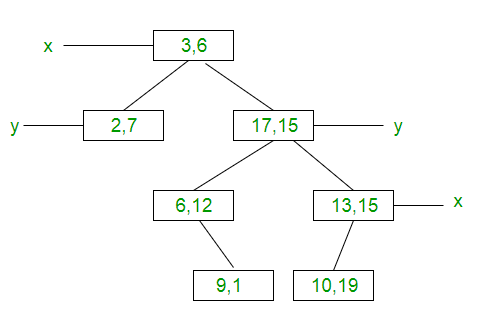
\includegraphics[width=300pt,height=180pt]{pictures/ktree_1.png}
    \caption{A demonstration of the \ac{KD}-tree algorithm with 7 datapoints having 2 dimensions x and y.\cite{kd_tree}}
    \label{fig:kd_tree}
\end{figure} 
At each level, the tree selects a dimension and splits the data points into two groups based on their values in that dimension. This process continues until all data points are assigned to leaf nodes. One of the key advantages of \ac{KD}-Trees lies in their ability to handle high-dimensional data in static dataset—a common challenge in machine learning applications like computer vision, natural language processing and bioinformatics. High-dimensional data often suffers from the “curse of dimensionality,” where the search space grows exponentially with the number of dimensions, making nearest neighbor queries time-consuming. As the ABC \cite{Koch_2019_CVPR} dataset is an immensely high dimensional dataset, the \ac{KD}-Tree algorithm is used in this use case. \ac{KD}-Trees address this by narrowing down the search space at each tree level, resulting in faster queries. Despite their advantages, \ac{KD}-Trees face limitations and challenges. One concern arises when the number of dimensions increases, particularly with non-uniformly distributed data points. In such cases, the tree may become unbalanced, resulting in inefficient search times. But since the datapoints are reduced to 2-dimensional datapoints, the \ac{HDBSCAN} algorithm doesn't result to inefficient search times in this case. Also \ac{KD}-trees are sensitive to outliers. The steps for \ac{KD}-tree algorithm are:
\begin{enumerate}
    \item \textbf{Dimension Selection}: A dimension is chosen along which the data is split \cite{friedman1975algorithm}.
    \item \textbf{Sorting}: The data points are sorted and arranged.
    \item \textbf{Median Point}: The median point (root of the current subtree) is selected, splitting the data into two subsets \cite{friedman1975algorithm}.
    \item \textbf{Recursive Process}: The process is repeated for each subset, with a new dimension selected at each level \cite{friedman1975algorithm}.
\end{enumerate}

\vspace{5mm}

\textbf{Ball-Tree algorithm}
The ball tree algorithm is designed for organizing and efficiently querying multidimensional data in computational geometry and machine learning. Formally, subsets of points are enclosed within hyperspheres and the structure is constructed as a binary tree. Each non-leaf node represents a hypersphere containing a subset of the data and each leaf node corresponds to a small subset of points. The partitioning process involves choosing a ‘pivotal’ point within the subset and constructing a hypersphere centered at this point to enclose the data as shown in Fig. \ref{fig:ball_tree}.
\begin{figure}[t]
    \centering
    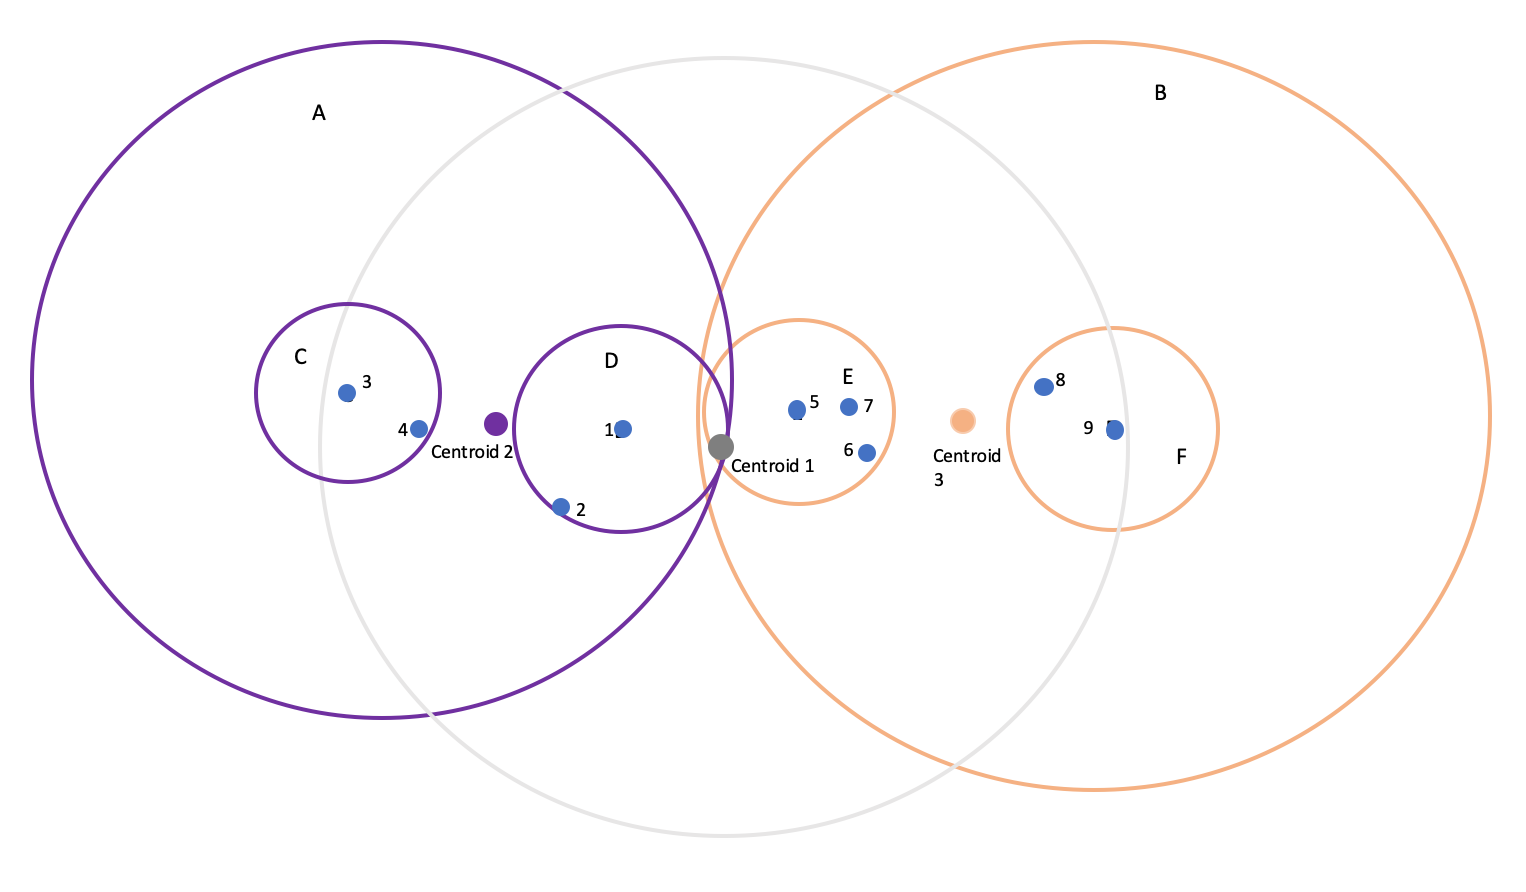
\includegraphics[width=300pt,height=180pt]{pictures/ball_tree.png}
    \caption{A demonstration of the Ball-tree algorithm with 9 datapoints having 2 dimensions x and y.\cite{kd_tree}}
    \label{fig:ball_tree}
\end{figure} 
Fast nearest neighbor searches are facilitated by this hierarchical arrangement, allowing for the rapid elimination of entire subtrees during the search process. Ball trees are particularly useful in scenarios with high-dimensional data, offering improved efficiency over exhaustive search methods in applications such as clustering, classification and nearest neighbor queries. The steps for ball-tree algorithm are:
\begin{enumerate}
    \item \textbf{Point Selection }: A random data point is chosen as the center of the hypersphere \cite{omohundro1989five}.
    \item \textbf{Radius Calculation}: The radius of the hypersphere is calculated using distance metrics such as Euclidean distance or Manhattan distance \cite{omohundro1989five}.
    \item \textbf{Datapoint Assignment}: Data points are assigned to the current node \cite{omohundro1989five}.
    \item \textbf{Recursive Process}: The process is repeated by selecting new centers and radii \cite{omohundro1989five}.
\end{enumerate}
Thus, the memory consumption for the ball-tree algorithm is way more in comparison to the \ac{KD}-tree algorithm. Furthermore, it fails to provide good results in low-dimensional data. It results to inefficient search time for low dimensional queries. This \ac{KD}-tree is suitable for low dimensional static use cases like image recognition and nearest neighbor search in low to medium dimensional dataset. Whereas, the ball tree algorithm is suitable for data clustering in high dimensional spaces and nearest neighbor search in high dimensional datasets.

\vspace{5mm}

\textbf{Brute Force Algorithm}
A brute force algorithm is a straightforward and exhaustive search strategy that systematically examines all possible options until it finds the solution to a problem. It’s a general approach used for problem-solving when the problem size allows for detailed investigation. In the brute force method, it is iterated through each data point and the density is calculated by considering the distances to other points. However, due to their high time complexity, brute force methods are inefficient for large-scale problems.

\subsection{Evaluation Metrices}
This section gives an overview of the evaluation metrices used to compare the results of the different clustering algorithms evaluated in this thesis. It also provides the details of the metric used to compare how similar the objects in the test dataset are to the representative members of the entire dataset. 
\subsubsection{Metric for Clustering Algorithms}
It is evident how even the evaluation metrics using just the intrinsic features of the dataset are still not efficient in the presence of noise, outliers or non-convex clusters. As pointed out by the authors of \cite{jain1988algorithms}, "without a strong effort in this direction, cluster analysis will remain a black art accessible only to those true believers who have experience and great courage". The fact that this statement holds even today, 35 years after he said it is even more astonishing. To tackle the problem of inefficient evaluation metrics for non-convex clusters or where the different clusters have a difference in size Moulavi \textit{et. al.} proposed the \ac{DBCV} Index \cite{moulavi2014density}.

\subsubsection*{Density Based Cluster Validition Index}
\label{sec:dbcv}
The authors have utilised the theory of Hartigan's model of density-contour trees \cite{hartigan1975clustering}. The least dense region within a cluster and the most dense region outside a cluster is calculated with it which is analogous to computing the within cluster and between cluster density connectedness. As per the definition of Density Contour Trees \cite{hartigan1975clustering} by Hartigan, density based clusters are regions of high density which are separated by low density regions. Having such model as a backdrop, it is expected that a good clustering algorithm which generate clusters such that the least dense region within a cluster is still more dense as compared to regions surrounding a cluster. Traditional intrinsic measure based evaluation metrics uses distance between the datapoints to compute cluster-variance and then incorporates it with the separation between the clusters to eventually compute the quality of the clustering algorithm. But this is not the target for \ac{DBCV}. So a metric is proposed which is defined by densities instead of distances. \ac{DBCV} wants to take into account both the density and the shape of the cluster. So at first, the authors defined the concept of "all-points-core-distance"($a_{pts}coredist$). It is the inverse of the density of each object with respect to all other objects inside its cluster as given in Eq. \ref{eq:aptscoredist}.
\begin{equation}
  \label{eq:aptscoredist}
  \mathit{a_{pts}coredist(\textbf{o})}= \mathit{\left\{\frac{\sum_{i=2}^{n_i}\left(\frac{1}{KNN(\textbf{o},i)}\right)^d}{n_i - 1}\right\}^{-\frac{1}{d}}}.
\end{equation}
Using the above-mentioned equation, a symmetric reachability distance is defined which is then utilized to generate the \ac{MST} inside each clusters. Because the \ac{MST}s are built on the transformed space of symmetric reachabilty distances, it is capable of capturing both the density and shape of the cluster. On using these \ac{MST}s, it is possible to find the least dense region within each of the clusters and the most dense regions between the pair of clusters. As per the definitions provided by the authors, $\textbf{O} = {o_1, o_2, ...., o_n}$ is the dataset containing $n$ objects in the $\mathbb{R}^d$ feature space. $\textbf{Dist}$ is an $n \times n$ matrix of pairwise distance $d(o_p,o_q)$ between the objects of the dataset, such that $o_p,o_q \in \textbf{O}$. $KNN(\textbf{o},i)$ is the distance between the object $o$ and its $i^{th}$ nearest neighbor. $C=({C_i},N) 1 \leq i \leq l$ is the results returned by the clustering algorithms having $l$ clusters and a set of $N$ noise objects. $n_i$ is the size of the $i^{th}$ cluster and $n_N$ is the number of objects in that particular cluster. To get an estimate of the density of an object within a cluster, traditional approaches use the notion of taking the inverse of the threshold distance required to find $K$ objects within this threshold \cite{hartigan1975clustering, campello2012simpler}. But a drawback of this method would be that it is required to decide the value of the parameter $K$, which is not desirable. 

\vspace{5mm}

Moreover, with this approach, the density of the object is dependent to its distance from only one other object i.e. the $k^th$ nearest neighbor. This approach is not as robust as compared to considering more objects in its neighborhood as done in Gaussian distribution kernel density estimation. Thus, in order to propose a more robust density estimation, the use of a new parameterless core distance is proposed which can be elucidated as the inverse of a density estimate and thus, can be used in defining the \ac{MRD}. So now instead of using just one point in the cluster, all the points are taken into account such that the objects closer to it contribute to the density more as compared to the objects further away. It can be seen in Eq. \ref{eq:aptscoredist}, that the inverse of the $KNN$ distances raised to the power of dimensions is calculated such that closer objects gets a higher weight as compared to further objects. This effect can further be increased by using squared Euclidean distance instead of Euclidean distances. Also, as per the definition of \ac{MRD}\cite{lelis2009semi}, the core distance of an object is compared to the distances of the object to other objects in the cluster. Hence, the core distance needs to be comparable to these distances. For each object $\textbf{o}$ in the cluster, the "all-points-core-distance" $a_{pts}coredist(\textbf{o})$ lies between the second and the last nearest neighbor distance of the object\cite{moulavi2014density} as in Eq. \ref{eq:knndist}. 

\begin{equation}
  \label{eq:knndist}
  \mathit{KNN(\textbf{o},2)} \leq \mathit{a_{pts}coredist(\textbf{o})} \leq \mathit{KNN(\textbf{o},n)}.
\end{equation}

Moreover, the core distance is approximated to the distance of the object to its $k^{th}$ nearest neighbor such that $k$ is not too large. This means, that only a small neighborhood of the object is to be considered. Furthermore, let n objects be uniformly distributed random variables in a d-dimensional unit hypersphere. Then the core distance of object $\textbf{o}$ is given by Eq. \ref{eq:aptsln}.\cite{moulavi2014density}

\begin{equation}
  \label{eq:aptsln}
  \mathit{a_{pts}coredist(\textbf{o})} = \mathit{\ln(n)^{-\frac{1}{d}}}.
\end{equation}

The core distance of the object $\textbf{o}$ is approximately equal to the same nearest neighbor distance and is independent of the dimension of the data space, if the objects are uniformly distributed. If the dataset doesn't have a uniform distribution, which is the case for most real world datasets, only the first property holds i.e. the density of the object doesn't depend on just one other object but on all objects in the cluster.\cite{moulavi2014density}

\vspace{5 mm}

Now the $a_{pts}coredist$ is used to compute the symmetric reachability distance which is delved into deeper in the following paragraphs. As per the authors, the \ac{MRD} between two objects $o_i$ and $o_j$ as in Eq. \ref{eq:mut_reach_dist}.

\begin{equation}
  \label{eq:mut_reach_dist}
  \mathit{d_{mreach}(\textbf{o}_i, \textbf{o}_j)} = \mathit{max\{a_{pts}coredist(\textbf{o}_i), a_{pts}coredist(\textbf{o}_j), d(\textbf{o}_i, \textbf{o}_j)\}},
\end{equation}

where $ d(\textbf{o}_i, \textbf{o}_j)$ is the Euclidean distance between object $\textbf{o}_i$ and $\textbf{o}_j$. Once the \ac{MRD} is computed, it could now be used to generate the mutual reachability graph where the objects are the different vertices and the graph and the \ac{MRD} calculated above are the edge weights between the pair of vertices. Now with the set of objects $\textbf{O}$ and the mutual reachability graph $G$, the \ac{MST} of graph $G$ is computed as $\ac{MST}_{\ac{MRD}}$. So a quick overview of the process of \ac{DBCV} would be that for a single cluster $C_i$ having objects $O$, the $a_{pts}coredist$ of each object in the cluster is calculated. This is then used to computer the \ac{MRD} between all pair of objects in the cluster. Depending on the \ac{MRD}, the \ac{MST} is generated. This process is then performed for all the clusters generated by the clustering algorithm, eventually giving rise to $l$ \ac{MST}s if the clustering algorithms returns $l$ clusters in total. Thus, it can noticed that the number of \ac{MST}s increase linearly with the increase in the number of clusters. Also, the size of the tree depends on the number of objects in the clusters and thus, can blow up exponentially in case of very large datasets having a lot of elements in each cluster.  

\vspace{5 mm}

From the \ac{MST}s generated above, a new measure to validate the quality of the clustering algorithm depending on the density sparseness and density separation is crafted as explained below. The \ac{DSC} $C_i$ can be visualized as the least dense region within the cluster and thus, can be obtained from the maximum edge weight of the $\ac{MST}_{\ac{MRD}}$ of that particular cluster. On the other hand, \ac{DSPC} $C_i$ and $C_j$ where $1 \leq i,j \leq l, i \neq j$  can be visualized as the region of highest density in between adjacent clusters and can be formulated as the minimum \ac{MRD} between the objects of a cluster to the objects of its neighboring cluster. The \ac{DSC} and the \ac{DSPC} together then give the validity index of a cluster as in Eq. \ref{eq:val_index}.
\begin{equation}
  \label{eq:val_index}
  \mathit{V_C(C_i)} = \mathit{\frac{\underset{1 \leq j \leq l, i \neq j}{min}\left(\ac{DSPC}(C_i,C_j)\right) - \ac{DSC}(C_i)}{max\left(\underset{1 \leq j \leq l, i \neq j}{min}\left(\ac{DSPC}(C_i,C_j)\right) - \ac{DSC}(C_i)\right)}}.
\end{equation}
Once the validity index of each cluster is calculated, the final \ac{DBCV} score of the clustering algorithm can be defined as the weighted average of the validity index of all the clusters in $C$ generated by the clustering algorithm as in Eq. \ref{eq:dbcv}. It is to be noted that even if noisy elements aren't explicitly present in the formula as a separate cluster but it does however implicitly affects the overall score as the weighted average takes into consideration both the cardinality of individual clusters as well as the total number of elements in the dataset, which includes noise and outliers. 
\begin{equation}
  \label{eq:dbcv}
  \mathit{\ac{DBCV}(C)} = \mathit{\sum_{i=1}^{l}\frac{|C_i|}{|O|}V_C(C_i)}.
\end{equation}
If a cluster has better density compactness within the cluster as compared to density separation in between adjacent clusters, than the validity index of the cluster would take a positive value. On the other hand, if the density outside the cluster separting it from adjacent clusters is more than density compactedness inside the cluster than it would take a negative value. Thus, the \ac{DBCV} score can vary in the range $[-1,1]$ where greater \ac{DBCV} score indicates to a better density-based clustering algorithm.

\subsubsection{Metric for Similarity in Point Clouds}
Hausdorff distance is commonly used to calculate the similarity between two point clouds. So if the set of representative members generalizes the entire dataset well enough, then each object in the test dataset would be very similar to atleast one object from the set of representative members. Hausdorff distance calculates how different one point cloud is to another. So, lower the Hausdorff distance, more similar are the point clouds to one another. Thus, for the a set of "good" representative members, the average distance from all objects in the test dataset to their corresponding nearest object in the representative set is minimum. Mathematically, Hausdorff distance is the measure of how far two subsets in a metric space. Intuitively speaking, the Hausdorff distance between two sets of points is lower when every point in one set is close to some point in the other set. In other words Hausdorff distance is the longest distance that needs to be covered when traveling from any point in one of the subsets to the closest point in the other subset. Let $(M,d)$ be a $d$-dimensional metric space and $X \subset M$, $Y \subset M$ are the two non-empty subsets of points, then the Hausdorff distance between $X$ and $Y$ is defined as in Eq. \ref{eq:hausdorff}.
\begin{equation}
    \label{eq:hausdorff}
    \mathit{d_H(X,Y)} := \mathit{\left\{max(\underset{x \in X}{sup} \; d(x,Y), \underset{y \in Y}{sup} \; d(X,y))\right\}},
  \end{equation}
where $sup$ is the supremum operator and $d(a,B) := \underset{b \in B}{inf} \; d(a,b)$ is the distance from a point $a \in X$ to the subset $B \subseteq X$, where $inf$ is the infimum operator. Thus, in the context of point clouds the Hausdorff distance is defined as in Eq. \ref{eq:hausdorff_point_cloud}. If $P_1 = \{x_i \in \mathbb{R}^3\}_{i=1}^n$ and $P_2 = \{x_j \in \mathbb{R}^3\}_{j=1}^m$, then the maximum distance between any pair of nearest neighbors between the two point clouds is defined as in eq. \ref{eq:hausdorff_point_cloud}.
\begin{equation}
    \label{eq:hausdorff_point_cloud}
    \mathit{hausdorff(P_1, P_2)} := \mathit{\frac{1}{2} \underset{x \in P_1}{max}\lvert x - NN(x,P_2) \rvert + \frac{1}{2} \underset{x' \in P_2}{max}\lvert x' - NN(x',P_1) \rvert},
  \end{equation}
\subsection{Important Aspects of the Studies}
\subsubsection{Focus and Restrictions}
\label{sec:restrictions}
The aim of this thesis is to find "good" representative members of the dataset which can be used as source library for transfer learning approaches to be used in bin picking applications. in order to do so, it is necessary to evaluate the performance of the clustering algorithms. But calculating the cluster evaluation metric like \ac{DBCV} for a very large high dimensional data can be extremely time consuming and inefficient. In order to circumvent this issue, the evaluation is carried on smaller subset of the dataset. But in order to ensure that the results can be interpolated to the entire dataset, subsets of varying sizes of the dataset have been evaluated on to confirm that the conclusions are consistent. The dimensions of the latent space representations play a very crucial role when encoding the features of the objects in a dataset in lower dimensional space. But in order to accurately evaluate the performance of the clustering algorithms, the number of dimensions has to be reduced further to be able to utilize the \ac{DBCV} metric for evaluation of the clustering results. Moreover, to facilitate larger but denser clusters \ac{t-SNE} dimensionality reduction is utilized. In the event of a rapid reduction of dimensions for example 1024 to 2, it is advised in \cite{tsne_sklearn} to perform multi-step dimensionality reduction instead of reducing it in a single step. This helps in better handling of the noise and outliers \cite{scikit-learn}. To assure that the theoretical advice is coherent with the practical results, evaluations are carried on in this area, the results of which are documented in Ch. \ref{sec:pointnet_dim} and \ref{sec:conclu_dim}. The data generation procedure currently used at \ac{IPA} requires 24 hours for completely generating a single object. It was decided to use 3 available servers for this purpose of data generation. A practical and feasible choice of roughly two months is made for this purpose. Two months nearly equals to 1400 hours. Thus, the underlying derivation shows how the maximum possible number of representative objects is determined.
\begin{equation}
    \label{eq:time_calc}
    \begin{split}
        Total \; time &= \frac{Number \; of \; clusters}{Number \; of \; servers} * Time \; for \; each \; object\\
        Number \; of \; clusters &= \frac{Total \; time \times Number \; of \; server}{Time \; for \; each \; object}
        \\
        &= \frac{1400 \times 3}{24} = 175
    \end{split}    
\end{equation}

\subsubsection{Hardware and Environment Setup}
\label{sec:hardware}
All the aspects of this thesis work has been carried on into a single setup, a powerful workstation computer, ML-Lab-2 at \ac{IPA}. It is an Ubuntu server. The \ac{CPU} are two ”Quad Core Intel Xeon Silver 4112 @ 2.60 GHz” with a total installed \ac{RAM} of 275 GB. The system has two \ac{GPU} which are "Tesla V100-PCIE-32GB" and "NVIDIA GeForce RTX 3090" with 32 \ac{GB} and 24 \ac{GB} memory respectively. Each of the individual model training is executed on a single GPU. 
\cleardoublepage




\section{Experiments}
\label{sec:experiments}
The two different backbone architecture for the generation of the latent space representation of the objects and the performance of the different clustering algorithms are evaluated by hyperparameter optimization of the different parameters along the entire pipeline of the procedure is evaluated in this section.

\subsection{Baseline Algorithm}
The already existing PointNet autoencoder currently used at \ac{IPA} is used as a baseline for evaluating the performance of the proposed algorithms in this thesis. The dimension of the output of the latent space representation of the baseline algorithm is 64. As mentioned in the restrictions in Section. \ref{sec:restrictions}, usually a two-step dimensionality reduction is performed before the datasets are grouped into clusters for the two networks evaluated in this thesis because the dimension of the output of the latent space representations is too high. This is done to suppress some noise and also to escalate the procedure by faster calculation of the pairwise distance between the datapoints. But since an output dimension of 64 is not very high, two-step dimensionality reduction is not necessary. However, to make the baseline algorithm comparable with the proposed networks, one-step dimensionality reduction is performed in some cases. 

\subsubsection{Basic Study without Dimensionality Reduction}
\label{sec:pointnet_dim}
Tab. \ref{tab:basic_without_tsne} shows the results of the baseline algorithm when no dimensionality reduction technique is used. It shows the results of the basic algorithm for the clustering of 1000 datapoints. The unit of time across all the tables in this section is in seconds unless otherwise mentioned. The four clustering algorithms \ac{HDBSCAN}, k-means clustering, spectral clustering and agglomerative clustering are evaluated. The number of clusters generated by the \ac{HDBSCAN} algorithm cannot be fixed by the user and hence it is determined by the algorithm automatically. Thus, the number of clusters after the first level of the multi-level \ac{HDBSCAN} algorithm as proposed in Section. \ref{sec:clustering_algo} is 232 in this case. As mentioned in Ch. \ref{sec:restrictions} the number of clusters for the rest of the clustering algorithms is set to 175 throughout all the experiments in this section. The \ac{DBCV} score caries in the range [-1,1] with more positive results denoting better clustering of the datapoints. The reason why \ac{HDBSCAN} algorithm shoes better results as compared to other clustering algorithms is \ac{HDBSCAN} algorithm is a density based clustering algorithm. \ac{DBCV} being a density based clustering validation index is likely to give better results for density based clustering algorithms which is proven to be true in this experiment. Furthermore, theoretically \ac{HDBSCAN} is better capable of handling noises and outliers in the dataset which can also contribute to the better results as exhibited in this experiment. 
\begin{table}[H]
    \setlength\extrarowheight{10pt}
    \caption{Results of the baseline algorithm on 1000 datapoints and without any dimensionality reduction technique. }
    \centering
    \begin{tabular}{|p{50pt}|p{60pt}|p{50pt}|p{40pt}|p{50pt}|p{40pt}|}
      \toprule
      No. of datapoints & Clustering Algorithm & No. of Clusters & Clustering Time (seconds) & \ac{DBCV} score & \ac{DBCV} Time (seconds)\\
      \midrule
      \multirow{4}{1.0in}{1000} & \ac{HDBSCAN} & 232 & 0.182 & -0.189 & 297.031 \\ \cline{2-6} 
                                & k-medoids & 175	& 3.960 & -0.332 & 237.640 \\ \cline{2-6} 
                                & Spectral & 175 & 2.396 & -0.339	& 161.604 \\ \cline{2-6}
                                & Agglomerative	& 175 & 0.115 & -0.327 & 157.584  \\ 
      \bottomrule
    \end{tabular}
    \label{tab:basic_without_tsne}
\end{table}

\subsubsection{Basic Study with T-distributed Stochastic Neighbor Embedding}
Tab. \ref{tab:basic_with_tsne} shows the results of the baseline algorithm when the \ac{t-SNE} dimensionality reduction is applied. The number of components for \ac{t-SNE} could be 1, 2 or 3 as per the available scikit-learn implementation \cite{scikit-learn}. It is set to be 2 in these set of experimentations for better and easier visualization. The \ac{DBCV} score caries in the range [-1,1] with more positive results denoting better clustering of the datapoints. The results are seen to be significantly better as compared to Tab. \ref{tab:basic_without_tsne} when dimensionality reduction technique is not applied. This is because the \ac{t-SNE} algorithm tends to keep datapoints that are distant from one another in the higher dimensional space also distant datapoints even in the lower-dimensional space. This gives rise to more dense and distinct clusters thus, improving the \ac{DBCV} score. As opposed to the result in Tab.\ref{tab:basic_without_tsne}, where the \ac{DBCV} score is negative, meaning the datapoints are mostly wrongly classification, in this table it can be seen that the datapoints are mostly correctly classified. It is also to be note that the number of clusters generated by the \ac{HDBSCAN} algorithm is 286 which is a bit more as compared to the previous case. This further hints to the direction that as a result of using \ac{t-SNE}, more dense and non-overlapping clusters are formed in the dataset. 
\begin{table}[H]
    \setlength\extrarowheight{10pt}
    \caption{Results of the baseline algorithm on 1000 datapoints after applying \ac{t-SNE} dimensionality reduction. }
    \centering
    \begin{tabular}{|p{30pt}|p{30pt}|p{40pt}|p{60pt}|p{50pt}|p{40pt}|p{30pt}|p{40pt}|}
      \toprule
      No. of datapoints & \ac{t-SNE} dim	& \ac{t-SNE} time (seconds) & Clustering Algorithm & No. of Clusters & Clustering Time (seconds) & \ac{DBCV} score & \ac{DBCV} Time (seconds)\\
      \midrule
      \multirow{4}{30pt}{1000} & 2	& 3.030 & \ac{HDBSCAN}	& 286	& 0.110 & 0.0975	& 275.039 \\ \cline{2-8} 
                                & 2	& 2.777 &	k-means	& 175	& 0.191 & -0.052  	& 94.004 \\ \cline{2-8} 
                                & 2	& 3.318 & Spectral	& 175	& 3.604 & -0.064 	& 126.854 \\ \cline{2-8}
                                & 2	& 3.190 & Agglomerative	& 175	& 0.087 & -0.076	& 113.937 \\ 
      \bottomrule
    \end{tabular}
    \label{tab:basic_with_tsne}
\end{table}
\subsubsection{Basic Study with Increasing Datapoints}
\begin{table}[H]
  \setlength\extrarowheight{10pt}
  \caption{Results of the baseline algorithm on 2000 datapoints and without any dimensionality reduction technique. }
  \centering
  \begin{tabular}{|p{50pt}|p{60pt}|p{50pt}|p{40pt}|p{50pt}|p{40pt}|}
    \toprule
    No. of datapoints & Clustering Algorithm & No. of Clusters & Clustering Time (seconds) & \ac{DBCV} score & \ac{DBCV} Time (seconds)\\
    \midrule
    \multirow{4}{1.0in}{2000} & \ac{HDBSCAN}	& 436	& 0.444 & -0.234	& 2115.777 \\ \cline{2-6} 
                              & k-medoids	& 175	& 0.793 & -0.462	& 764.222 \\ \cline{2-6} 
                              & Spectral	& 175	& 20.607 & -0.617	& 749.487 \\ \cline{2-6}
                              & Agglomerative	& 175	& 0.205 & -0.502	& 756.480 \\ 
    \bottomrule
  \end{tabular}
  \label{tab:basic_2000_without_tsne}
\end{table}
As mentioned in Ch. \ref{sec:restrictions}, it is extremely inefficient to compute the \ac{DBCV} for all the datapoints in the ABC datasets \cite{Koch_2019_CVPR} as once. It is necessary to verify that the results obtained for a smaller subset of the dataset can be interpolated for the entire dataset. In other words, the results obtained for a smaller subset of the dataset generalizes the behavior of the entire dataset well. Tab. \ref{tab:basic_2000_without_tsne} shows the results of the baseline algorithm on 2000 datapoints without applying dimensionality reduction and Tab. \ref{tab:basic_2000_with_tsne} shows the results of the baseline algorithm on 2000 datapoints when \ac{t-SNE} dimensionality reduction is applied. It is observed that roughly $10\%$ of the datapoints are classified as outliers by the \ac{HDBSCAN} algorithm for all the experiments on 1000 and 2000 datapoints. 

\begin{table}[H]
    \setlength\extrarowheight{10pt}
    \caption{Results of the baseline algorithm on 2000 datapoints after applying \ac{t-SNE} dimensionality reduction. }
    \centering
    \begin{tabular}{|p{30pt}|p{30pt}|p{40pt}|p{60pt}|p{50pt}|p{40pt}|p{30pt}|p{40pt}|}
      \toprule
      No. of datapoints & \ac{t-SNE} dim	& \ac{t-SNE} time & Clustering Algorithm & No. of Clusters & Clustering Time (seconds) & \ac{DBCV} score & \ac{DBCV} Time (seconds)\\
      \midrule
      \multirow{4}{30pt}{2000} & 2	& 6.689 & \ac{HDBSCAN}	& 626	& 0.237 & 0.172	& 4497.151 \\ \cline{2-8} 
                                & 2	& 7.450 & k-medoids	& 175	& 0.155 & -0.226 &	932.509 \\ \cline{2-8} 
                                & 2	& 157.017& Spectral	& 175	& 91.684 & -0.125 & 755.647 \\ \cline{2-8}
                                & 2	&  5.155 & Agglomerative & 175 & 0.112 & -0.192 & 363.605 \\ 
      \bottomrule
    \end{tabular}
    \label{tab:basic_2000_with_tsne}
\end{table}

\subsection{ConClu Approach with PointNet as Backbone}
\label{sec:conclu_with_pointnet}
As mentioned in Ch. \ref{sec:method}, two feature representation learning backbones are used for the experiments. Experiments with the PointNet autoencoder as the backbone is recorded here. The performance of all the clustering algorithm is evaluated. Different hyperparameter optimizations are performed which will be elaborated  gradually through this subsection.  

\subsubsection{Evaluation of Increasing Datapoints}
\label{sec:conclu_with_inc_data}
\begin{table}[H]
  \setlength\extrarowheight{10pt}
  \caption{Results of the ConClu approach on 1000 datapoints. }
  \centering
  \begin{tabular}{|p{50pt}|p{60pt}|p{50pt}|p{40pt}|p{50pt}|p{40pt}|}
    \toprule
    No. of datapoints & Clustering Algorithm & No. of Clusters & Clustering Time (seconds) & \ac{DBCV} score & \ac{DBCV} Time (seconds)\\
    \midrule
    \multirow{4}{1.0in}{1000} & \ac{HDBSCAN}	& 288	& 0.228 & 0.137	& 437.956 \\ \cline{2-6} 
                              & Agglomerative	& 175	& 0.063 & -0.057	& 191.887 \\ \cline{2-6} 
                              & k-medoids	& 175	& 0.763 & -0.120 	& 192.580 \\ \cline{2-6}
                              & Spectral	& 175	& 7.831 & -0.051	& 186.879 \\ 
    \bottomrule
  \end{tabular}
  \label{tab:conclu_1000}
\end{table}
As mentioned in Ch. \ref{sec:restrictions}, it is extremely inefficient to compute the \ac{DBCV} for all the datapoints in the ABC datasets \cite{Koch_2019_CVPR} as once. It is necessary to verify that the results obtained for a smaller subset of the dataset can be interpolated for the entire dataset. In other words, the results obtained for a smaller subset of the dataset generalizes the behavior of the entire dataset well. Tab. \ref{tab:conclu_1000} shows the results of the ConClu approach on 1000 datapoints and Tab. \ref{tab:conclu_2000}  and \ref{tab:conclu_5000} shows the results of the ConClu approach on 2000 datapoints and 5000 datapoints respectively. It is observed that roughly $10\%$ of the datapoints are classified as outliers by the \ac{HDBSCAN} algorithm for all the experiments on 1000, 2000 and 5000 datapoints. The dimension of the latent space representations for table
\ref{tab:conclu_1000}, \ref{tab:conclu_2000} and \ref{tab:conclu_5000} is 1024. 

\begin{table}[H]
  \setlength\extrarowheight{10pt}
  \caption{Results of the ConClu approach on 1000 datapoints for multi-level \ac{HDBSCAN} clustering algorithm. }
  \centering
  \begin{tabular}{|l|l|l|l|l|p{40pt}|}
    \toprule
    Level & Algorithm	& No. of Clusters	& No. of Outliers	& DBCV score	& DBCV Time (seconds)	\\  
    \midrule
    Level 1 & \ac{HDBSCAN}	& 288	& 94	& 0.137	& 437.956 \\ \cline{1-6}
    Level 2 & \ac{HDBSCAN}	& 111	& 33	& -0.023	& 113.242 \\ 

    \bottomrule
  \end{tabular}
  \label{tab:conclu_1000_levels}
\end{table}

 Tab. \ref{tab:conclu_1000_levels} shows the performance of the multi-level \ac{HDBSCAN} algorithm for 1000 datapoints. The performance of this algorithm is seen to deteriorate as compare to the traditional \ac{HDBSCAN} algorithm. This is because, clusters are combined to form bigger clusters in this algorithm to limit the number of maximum clusters returned by it. But it is still seen to perform better as compared to other traditional clustering algorithm like k-medoids, spectral clustering and agglomerative clustering. The next best clustering algorithm in this case is spectral clustering. It is also to be noted that the clustering time even for multiple levels in multi-level \ac{HDBSCAN} algorithm is less than that of spectral clustering algorithm by quite some factors. The number of outliers after the first level denotes the number of datapoints that is newly classified as outlier which is not classified as outliers in the previous layer. These new outliers and its associated cluster members are then re-assigned as a new cluster. Thus, outliers of the dataset remains constant after the first iteration of the multi-level \ac{HDBSCAN} clustering algorithm. This means, more information is not lost and no new datapoint is classified as an outlier. This is necessary to ensure that not too many objects in the dataset is discarded as outliers and the representative members at the end is actually a general representative of almost the entire dataset. 

\begin{table}[H]
  \setlength\extrarowheight{10pt}
  \caption{Results of the ConClu approach on 2000 datapoints. }
  \centering
  \begin{tabular}{|p{50pt}|p{60pt}|p{50pt}|p{40pt}|p{50pt}|p{40pt}|}
    \toprule
    No. of datapoints & Clustering Algorithm & No. of Clusters & Clustering Time (seconds) & \ac{DBCV} score & \ac{DBCV} Time (seconds)\\
    \midrule
    \multirow{4}{1.0in}{2000} & \ac{HDBSCAN}	& 605	& 1.030 & 0.159	& 8278.394 \\ \cline{2-6} 
                              & Agglomerative	& 175	& 0.196 & -0.212	& 786.866 \\ \cline{2-6} 
                              & k-medoids	& 175	& 6.322 & -0.209	& 1079.195 \\ \cline{2-6}
                              & Spectral	& 175	& 80.008 & -0.145	& 1187.477 \\ 
    \bottomrule
  \end{tabular}
  \label{tab:conclu_2000}
\end{table}

It can be noticed that the \ac{DBCV} score for the \ac{HDBSCAN} algorithm increases consistently from 1000 datapoints to 2000 datapoints and so on. This could be attributed to the fact that more datapoints would quite naturally give rise to denser clusters. More dense the inside of the cluster is as compared to its outside, the better is the \ac{DBCV} score. This further reassures the fact that denser clusters would mean more number of elements in individual clusters. In other words, the representative member of the cluster would represent a more diverse amount of other cluster members. 

\begin{table}[H]
  \setlength\extrarowheight{10pt}
  \caption{Results of the ConClu approach on 5000 datapoints. }
  \centering
  \begin{tabular}{|p{50pt}|p{60pt}|p{50pt}|p{40pt}|p{50pt}|p{50pt}|}
    \toprule
    No. of datapoints & Clustering Algorithm & No. of Clusters & Clustering Time (seconds) & \ac{DBCV} score & \ac{DBCV} Time (seconds)\\
    \midrule
    \multirow{4}{1.0in}{5000} & \ac{HDBSCAN}	& 1.586	& 1.904 & 0.210	& 165884.854 \\ \cline{2-6} 
                              & Agglomerative	& 175	& 1.345 & -0.380	& 4945.410 \\ \cline{2-6} 
                              & k-medoids	& 175	& 9.142 & -0.427	& 8289.148 \\ \cline{2-6}
                              & Spectral	& 175	& 641.189 & -0.359	& 5069.388 \\ 
    \bottomrule
  \end{tabular}
  \label{tab:conclu_5000}
\end{table}

Also it is noteworthy how the time to calculate the \ac{DBCV} score doesn't increase linearly on increasing the number of datapoints. Rather it increases in an exponential rate. This shows how it would take immensely long to compute the \ac{DBCV} score of the entire dataset in the presence of one million datapoints in it. But since the results obtained on a smaller subset of the dataset can be interpolated to the entire dataset, evaluation hyperparameter optimization for the rest of the parameters are performed on 1000 datapoints. However, after deciding the final values for all the hyperparameters, the cluster representatives are generated taking into account all the datapoints under consideration as that no longer involves calculating the \ac{DBCV} score anymore for evaluation.  

\subsubsection{Evaluation of Different Dimensionality Reduction Techniques}
\label{sec:conclu_dim}
As mentioned in Ch. \ref{sec:restrictions}, it is essential to perform dimensionality reduction before clustering the objects in the dataset into groups. Two different dimensionality techniques are evaluated for this purpose, the \ac{PCA} method and the \ac{t-SNE} method. 
\begin{table}[H]
  \setlength\extrarowheight{10pt}
  \caption{Results of the ConClu approach with PointNet autoencoder on 1000 datapoints with \ac{PCA} as dimensionality reduction technique in both steps. }
  \centering
  \begin{tabular}{|p{30pt}|p{30pt}|p{30pt}|p{30pt}|p{60pt}|p{30pt}|p{40pt}|p{30pt}|p{30pt}|}
    \toprule
    \ac{PCA} dim & \ac{PCA} time (seconds) & \ac{PCA} dim	& \ac{PCA} time (seconds) & Clustering Algorithm & No. of Clusters & Clustering Time (seconds) & \ac{DBCV} score & \ac{DBCV} Time (seconds)\\
    \midrule
    \multirow{4}{30pt}{512}	& 32.921 & 154	& 11.249 & \ac{HDBSCAN}	& 169	& 0.459 & -0.410	& 234.172 \\ \cline{2-9} 
                              & 41.230 & 154	& 14.891 & Agglomerative	& 175	& 0.216 & -0.151	& 209.954 \\ \cline{2-9} 
                              & 38.408 & 154	& 13.032 & k-medoids	& 175	& 7.001 & -0.184	& 212.482 \\ \cline{2-9}
                              & 44.171 & 154	& 13.897 & Spectral	& 175	& 46.703 &-0.481 & 221.064 \\ 
    \bottomrule
  \end{tabular}
  \label{tab:conclu_pca_1000}
\end{table}
Tab. \ref{tab:conclu_pca_1000} shows the results on the ConClu approach for 1000 datapoints and applying \ac{PCA} method as the dimensionality reduction technique in both steps. As the \ac{DBCV} score depends on the number of nearest neighbor raised to the power of the negative of one divided by the number of features in the latent space representation as shown in Eq. \ref{eq:aptscoredist} on Pg. 48, it is important to determine the to the maximal possible dimension of the representation after the second step of dimensionality reduction. Experiments are performed and the value is found to be 154 in this use case. Also keeping the first step of dimensionality reduction to be \ac{PCA}, experiments are also conducted with \ac{t-SNE} method as the second step. Tab. \ref{tab:conclu_tsne_1000} shows the results on the ConClu approach for 1000 datapoints under such settings. The dimensions of the latent space representations in both the cases is set to 1024. it is to be noted that the results for all the clustering algorithms have better performance when \ac{t-SNE} is used as the dimensionality reduction technique in the second step as compared to \ac{PCA}. It can be attributed to the fact that the \ac{t-SNE} algorithm preserves the spatial relationship between the datapoints. In other words, if datapoints are close to one another in a higher dimensional space, \ac{t-SNE} tends to preserve this spatial closeness between points even in the lower dimensional space. 

\begin{table}[H]
  \setlength\extrarowheight{10pt}
  \caption{Results of the ConClu approach with PointNet autoencoder on 1000 datapoints with \ac{PCA} as dimensionality reduction technique in the first step and \ac{t-SNE} as the second. }
  \centering
  \begin{tabular}{|p{30pt}|p{30pt}|p{30pt}|p{30pt}|p{60pt}|p{30pt}|p{40pt}|p{30pt}|p{30pt}|}
    \toprule
    \ac{PCA} dim & \ac{PCA} time (seconds) & \ac{t-SNE} dim	& \ac{t-SNE} time (seconds) & Clustering Algorithm & No. of Clusters & Clustering Time (seconds) & \ac{DBCV} score & \ac{DBCV} Time (seconds)\\
    \midrule
    \multirow{4}{30pt}{512}	& 32.530 & 2	& 143.024 & \ac{HDBSCAN}	& 288	& 0.228 & 0.137	& 437.956 \\ \cline{2-9} 
                              & 38.832 & 2	& 141.566 & Agglomerative & 175	& 0.063 & -0.057 & 191.887 \\ \cline{2-9} 
                              & 39.326 & 2	& 162.957 & k-medoids	& 175	& 7.763 & -0.120 	& 192.580 \\ \cline{2-9}
                              & 71.552 & 2	& 177.427 & Spectral	& 175	& 28.831 & -0.051	& 186.879 \\ 
    \bottomrule
  \end{tabular}
  \label{tab:conclu_tsne_1000}
\end{table}

Also it is to be noted that the \ac{HDBSCAN} algorithm performs significantly bad in presence of \ac{PCA} as compared to \ac{t-SNE} as the second step of dimensionality reduction. This is also because of the property of \ac{t-SNE} mentioned above which gives rise to denser clusters as compared to \ac{PCA}.  

\begin{table}[H]
  \setlength\extrarowheight{10pt}
  \caption{Results of the ConClu approach with PointNet autoencoder on 1000 datapoints with only \ac{t-SNE} as dimensionality reduction technique as the only  step. }
  \centering
  \begin{tabular}{|p{30pt}|p{30pt}|p{30pt}|p{60pt}|p{50pt}|p{40pt}|p{30pt}|p{30pt}|}
      \toprule
      No. of datapoints & \ac{t-SNE} dim	& \ac{t-SNE} time (seconds) & Clustering Algorithm & No. of Clusters & Clustering Time (seconds) & \ac{DBCV} score & \ac{DBCV} Time (seconds)\\
      \midrule
      \multirow{4}{30pt}{1000} & 2	& 6.769 & \ac{HDBSCAN}	& 314	& 0.189 & -0.120 & 337.313 \\ \cline{2-8} 
                                & 2	& 4.872 & k-medoids	& 175	& 0.337 & -0.132
                                & 131.622 \\ \cline{2-8} 
                                & 2	& 5.831	& Spectral	& 175	& 7.592 & -0.122	& 130.678 \\ \cline{2-8}
                                & 2	& 4.478 & Agglomerative	& 175	& 0.033 & -0.085 & 128.358 \\ 
      \bottomrule
  \end{tabular}
  \label{tab:conclu_1000_without_reduction}
\end{table}

The effect of two step dimensionality reduction is also compared against only one step dimensionality reduction as shown in Tab. \ref{tab:conclu_1000_without_reduction}. A \ac{PCA} followed by a \ac{t-SNE} shows better results as compared to directly applying \ac{t-SNE} just once. This is because of the fact that a multi-step dimensionality reduction helps in reducing the noises during the procedure. Thus, for the rest of the experiments the dimensionality reduction with \ac{PCA} having number of components to be 512 in the first step is performed followed by applying the \ac{t-SNE} method with 2 components as the next step. 

\subsubsection{Evaluation of Dimension of Feature Space Representations}
Latent space representations are lower dimensional representations of the dataset. It is expensive to work with very high dimensional data. Thus, the dimension of the latent space representations is immensely important. It is necessary that the original high dimensional data is compressed to a lower dimensional latent space without severe loss of information in the process. Since the original dataset has the point clouds with 2048, for the sake of completeness of the experimentation, the evaluation is performed for all dimensions on a logarithmic scale of 2 from 2048 to down until 4. Tab. \ref{tab:conclu_2048} shows the experiments when the dimension of the latent space representations is set to be 2048. As mentioned in Ch. \ref{sec:restrictions}, because of the very high number of features in the output of the network, a two-step dimensionality reduction is performed to suppress noise during the process of dimensionality reduction and also to facilitate faster calculation of the pairwise distance between the points. In line with the results of the previous experiments, the \ac{HDBSCAN} clustering algorithm produces the best results. The learning rate is rate set to 0.001 with a decay factor of 0.1 throughout all the experiments in this subsection. A early stopping criteria is used to naturally terminate the training of the models on convergence. When the validation loss no long reduced for atleast 5 epochs, then the training is terminated. The number of epochs is set to a very high number of 200 for all the experiments so that the training is only stopped when early stopping criteria is triggered on model convergence. 
\begin{table}[H]
    \setlength\extrarowheight{10pt}
    \caption{Results of the ConClu approach with PointNet autoencoder on 1000 datapoints when the dimensions of the latent space representations is 2048. }
    \centering
    \begin{tabular}{|p{30pt}|p{30pt}|p{30pt}|p{30pt}|p{60pt}|p{30pt}|p{40pt}|p{30pt}|p{30pt}|}
      \toprule
      \ac{PCA} dim & \ac{PCA} time (seconds)& \ac{t-SNE} dim	& \ac{t-SNE} time (seconds) & Clustering Algorithm & No. of Clusters & Clustering Time (seconds) & \ac{DBCV} score & \ac{DBCV} Time (seconds)\\
      \midrule
      \multirow{4}{30pt}{512}	& 18.507 & 2	& 3.594 & \ac{HDBSCAN}	& 289	& 0.127 & 0.189 & 243.297 \\ \cline{2-9} 
      & 15.525 & 2	& 3.368 & Agglomerative	& 175	& 0.036	& -0.013	& 109.668 \\ \cline{2-9} 
      & 16.595 & 2	& 3.709 & k-medoids & 175	& 0.222 & -0.040	& 102.518 \\ \cline{2-9}
      & 18.593 & 2	& 3.918 & Spectral	& 175	& 9.257 & 0.020	& 101.925 \\ 
      \bottomrule
    \end{tabular}
    \label{tab:conclu_2048}
\end{table}

\begin{table}[H]
  \setlength\extrarowheight{10pt}
  \caption{Results of the ConClu approach on 1000 datapoints for multi-level \ac{HDBSCAN} clustering algorithm when the dimensions of the latent space representations is 2048. }
  \centering
  \begin{tabular}{|l|l|l|l|l|l|}
    \toprule
    Level & Algorithm	& No. of Clusters	& No. of Outliers	& DBCV score	& \ac{DBCV} time (seconds)	\\  
    \midrule
    Level 1 & \ac{HDBSCAN}	& 289	& 105	& 0.189 & 243.297 \\ \cline{1-6}
    Level 2 & \ac{HDBSCAN}	& 127	& 53	& 0.021	& 65.340
    \\ 
    \bottomrule
  \end{tabular}
  \label{tab:conclu_2048_levels}
\end{table}

As observed in Ch. \ref{sec:conclu_with_inc_data}, in Tab. \ref{tab:conclu_2048_levels} too it can be seen that the performance of multi-level \ac{HDBSCAN} algorithm deteriorates as compared to \ac{HDBSCAN} but it is still comparable to spectral clustering and better than the rest. But larger dimensions of the latent space representations mean longer training time. When it is set to 2048, the model converges after the $50^{th}$ epoch according to the early stopping criteria mentioned above with a total training time of 137.4 hours which is quite high. So to evaluate the performance of the model with fewer dimensions of the latent space representations further experiments are conducted. Tab. \ref{tab:conclu_tsne_1000} and \ref{tab:conclu_512} shows the experiments when the dimension of the latent space representations is set to be 1024 and 512 respectively. The number of semantic subgroups or parts in the objects is set to 64 in line with \cite{mei2022unsupervised} to find the optimum number of dimensions of the latent space representations. Experiments on the number of semantic subgroups are included in Ch. \ref{sec:conclu_pointnet_semantic}. 

\begin{table}[H]
  \setlength\extrarowheight{10pt}
  \caption{Results of the ConClu approach with PointNet autoencoder on 1000 datapoints when the dimension of the latent space representations is 512. }
  \centering
  \begin{tabular}{|p{30pt}|p{50pt}|p{60pt}|p{50pt}|p{50pt}|p{50pt}|p{40pt}|}
    \toprule
    \ac{t-SNE} dim	& \ac{t-SNE} time & Clustering Algorithm & No. of Clusters & Clustering Time (seconds) & \ac{DBCV} score & \ac{DBCV} Time (seconds)\\
    \midrule
    \multirow{4}{30pt}{2}	& 145.809 & \ac{HDBSCAN}	& 307	& 0.187 & 0.186	& 489.133 \\ \cline{2-7} 
    & 6.575 & k-medoids	& 175	& 0.532 & -0.023	& 129.956 \\ \cline{2-7} 
    & 4.989 & Spectral	& 175	& 9.226 & 0.024 & 131.239 \\ \cline{2-7}
    & 6.823 & Agglomerative	& 175	& 0.053 & 0.010 & 131.956 \\ 
    \bottomrule
  \end{tabular}
  \label{tab:conclu_512}
\end{table}

\begin{table}[H]
  \setlength\extrarowheight{10pt}
  \caption{Results of the ConClu approach on 1000 datapoints for multi-level \ac{HDBSCAN} clustering algorithm when the dimensions of the latent space representations is 512. }
  \centering
  \begin{tabular}{|l|l|l|l|l|l|}
    \toprule
    Level & Algorithm	& No. of Clusters	& No. of Outliers	& DBCV score	& \ac{DBCV} time (seconds)	\\  
    \midrule
    Level 1 & \ac{HDBSCAN}	& 307 & 93 & 0.186	& 489.133  \\ \cline{1-6}
    Level 2 & \ac{HDBSCAN}	& 126	& 38	& 0.024	& 129.881  \\ 
    \bottomrule
  \end{tabular}
  \label{tab:conclu_512_levels}
\end{table}

Similarly, Tab. \ref{tab:conclu_512_levels} records the performance of the multi-level \ac{HDBSCAN} algorithm. In line with the previous observations, the results direct to similar conclusions in this case well with \ac{HDBSCAN} algorithm having the best result followed by multi-level \ac{HDBSCAN} and spectral clustering algorithm having comparable results with a large difference in the clustering time. The training time for the model with 1024 dimensions is 73 hours for 65 epochs. The training time for the model with 512 dimensions is 64 hours for 54 epochs. The performance for the model with dimension 512 is comparable to the model with dimension 2048 for a much lower training time. If a good enough result could be achieved with a significant decrease in the training time, it would mean a more cost efficient model. It is to be noted here that the performance of the \ac{HDBSCAN} algorithm is worse for dimension 1024 as compared to both dimensions 2048 and 512. To achieve a conclusive result as to whether the performance of the \ac{HDBSCAN} algorithm on the model with dimension 1024 is an outlier, further experiments are conducted to train models with fewer dimensions. Tab. \ref{tab:conclu_256} and Tab. \ref{tab:conclu_128} are the experiments for the model with dimensions 256 and 128 respectively with rest of the parameters being same as mentioned above. Tab. \ref{tab:conclu_256_levels} shows the performance of the multi-level \ac{HDBSCAN} algorithm when the model ad dimension 256. The training time for the model with dimension 256 is 42 hours for 50 epochs. 

\begin{table}[H]
  \setlength\extrarowheight{10pt}
  \caption{Results of the ConClu approach with PointNet autoencoder on 1000 datapoints when the dimension of the latent space representations is 256. }
  \centering
  \begin{tabular}{|p{30pt}|p{50pt}|p{60pt}|p{50pt}|p{50pt}|p{50pt}|p{40pt}|}
    \toprule
    \ac{t-SNE} dim	& \ac{t-SNE} time & Clustering Algorithm & No. of Clusters & Clustering Time (seconds) & \ac{DBCV} score & \ac{DBCV} Time (seconds)\\
    \midrule
    \multirow{4}{30pt}{2}	& 5.901 & \ac{HDBSCAN}	& 293	& 0.725 & 0.164	& 718.808 \\ \cline{2-7} 
    & 6.206 & k-medoids	& 175	& 0.471	& -0.078	& 136.173 \\ \cline{2-7} 
    & 6.106 & Spectral	& 175	& 11.077 & 0.003	& 133.593 \\ \cline{2-7}
    & 5.539 & Agglomerative	& 175	& 0.031 & -0.020	& 132.193 \\ 
    \bottomrule
  \end{tabular}
  \label{tab:conclu_256}
\end{table}

Whereas, the training time for the model with dimension 256 is 32 hours for 40 epochs. It is observed that there is no significant change in the training time as compared to training time of the model with dimension of 512 to 256 as it is observed when the dimension changed from 2048 to 512. In the latter, when the dimension changed by a factor of 4, the training time reduced by almost a factor of 2.

\begin{table}[H]
  \setlength\extrarowheight{10pt}
  \caption{Results of the ConClu approach on 1000 datapoints for multi-level \ac{HDBSCAN} clustering algorithm when the dimensions of the latent space representations is 256. }
  \centering
  \begin{tabular}{|l|l|l|l|l|l|}
    \toprule
    Level & Algorithm	& No. of Clusters	& No. of Outliers	& DBCV score	& \ac{DBCV} time (seconds)	\\  
    \midrule
    Level 1 & \ac{HDBSCAN}	& 293	& 95	& 0.164	& 718.808 \\ \cline{1-6}
    Level 2 & \ac{HDBSCAN}	& 122	& 41	& 0.045	& 198.859 \\ 
    \bottomrule
  \end{tabular}
  \label{tab:conclu_256_levels}
\end{table}

\begin{table}[H]
  \setlength\extrarowheight{10pt}
  \caption{Results of the ConClu approach with PointNet autoencoder on 1000 datapoints when the dimension of the latent space representations is 128. }
  \centering
  \begin{tabular}{|p{30pt}|p{50pt}|p{60pt}|p{50pt}|p{50pt}|p{50pt}|p{40pt}|}
    \toprule
    \ac{t-SNE} dim	& \ac{t-SNE} time & Clustering Algorithm & No. of Clusters & Clustering Time (seconds) & \ac{DBCV} score & \ac{DBCV} Time (seconds)\\
    \midrule
    \multirow{4}{30pt}{2}	& 3.036 & \ac{HDBSCAN}	& 307	& 0.121 & 0.174	& 354.460 \\ \cline{2-7} 
    & 3.689 & k-medoids	& 175	& 5.255 & -0.037	& 177.251 \\ \cline{2-7} 
    & 3.295 & Spectral	& 175	& 5.511 & 0.024	& 116.696 \\ \cline{2-7}
    & 3.531 & Agglomerative	& 175	& 0.057 & -0.033	& 94.799 \\ 
    \bottomrule
  \end{tabular}
  \label{tab:conclu_128}
\end{table}

Whereas, when the dimension changed from 512 to 128, there is a change in the dimension by a factor of 4 but the training time does not reduce comparably. Also, the performance of the \ac{HDBSCAN} algorithm is better with the model of dimension 512 by $2\%$ and $1\%$ as compared to models with dimension 256 and 128 respectively. Until now, the number of semantic subgroups in the objects are set to 64. In other words, each dimension of the feature representation of the point cloud is to belong to 1 of the 64 semantic subgroups or parts. Thus, when the dimension of of the latent space representation of the objects is atmost 64, it is not realistic to have 64 semantic subgroups. So to train the models with dimensions of latent space representation to be less than equal to 64, the number of semantic subgroups is to chosen to be half of the number of dimensions. So the model of dimension 64 has K set to be 32, the model of dimensions 32 has K set to be 16 and so on. 
Thus, Tab. \ref{tab:conclu_64} and Tab. \ref{tab:conclu_32} are the experiments for the model with dimensions 256 and 128 respectively with rest of the parameters being same as mentioned above. The training time for the model with 64 dimensions is 45 hours for 48 epochs. The training time for the model with 32 dimensions is 23 hours for 39 epochs.

\begin{table}[H]
  \setlength\extrarowheight{10pt}
  \caption{Results of the ConClu approach with PointNet autoencoder on 1000 datapoints when the dimension of the latent space representations is 64. }
  \centering
  \begin{tabular}{|p{30pt}|p{50pt}|p{60pt}|p{50pt}|p{50pt}|p{50pt}|p{40pt}|}
    \toprule
    \ac{t-SNE} dim	& \ac{t-SNE} time & Clustering Algorithm & No. of Clusters & Clustering Time (seconds) & \ac{DBCV} score & \ac{DBCV} Time (seconds)\\
    \midrule
    \multirow{4}{30pt}{2}	& 3.059 & \ac{HDBSCAN}	& 286	& 0.538 & 0.148 	& 639.097 \\ \cline{2-7} 
    & 3.086 & k-medoids	& 175	& 3.143 & -0.068	& 145.711 \\ \cline{2-7} 
    & 3.189 & Spectral	& 175	& 8.760 & -0.020	& 152.836 \\ \cline{2-7}
    & 3.914 & Agglomerative	& 175	& 0.032 & -0.017	& 157.152 \\ 
    \bottomrule
  \end{tabular}
  \label{tab:conclu_64}
\end{table}

As expected, the performance of these models have decreased by $4\%$ and $3\%$ respectively as compared to the model with dimensions 512. When the number of dimensions have decreased by a factor of 16, the amount of training time has only reduced by a factor of 3 when the dimensions have change from 512 to 32. The learning rate for all the experiments in this subsection is set to 0.001 with a decay factor of 0.1. A batch size of 128 is chosen for these experiments as that is the maximum possible batch size that could be executed without running into out of memory issues in the given hardware setup. 

\begin{table}[H]
  \setlength\extrarowheight{10pt}
  \caption{Results of the ConClu approach with PointNet autoencoder on 1000 datapoints when the dimension of the latent space representations is 32. }
  \centering
  \begin{tabular}{|p{30pt}|p{50pt}|p{60pt}|p{50pt}|p{50pt}|p{50pt}|p{40pt}|}
    \toprule
    \ac{t-SNE} dim	& \ac{t-SNE} time & Clustering Algorithm & No. of Clusters & Clustering Time (seconds) & \ac{DBCV} score & \ac{DBCV} Time (seconds)\\
    \midrule
    \multirow{4}{30pt}{2}	& 2.748 & \ac{HDBSCAN}	& 273	& 0.222 & 0.158	& 562.223 \\ \cline{2-7} 
    & 2.917 & k-medoids	& 175	& 1.434 & -0.021	& 141.890 \\ \cline{2-7} 
    & 2.985 & Spectral	& 175	& 6.190 & 0.016	& 107.808 \\ \cline{2-7}
    & 2.501 & Agglomerative	& 175	& 0.031 & 0.023	& 93.092 \\ 
    \bottomrule
  \end{tabular}
  \label{tab:conclu_32}
\end{table}

Experiments are also conducted for training the models with dimensions 16, 8 and 4 for the completeness of the experiments. Since the dimensions of the latent space representations are to be categorized into subgroups, the minimum number of possible subgroups is 2. Therefore, a model with the dimension of the latent space representations as 2 is not realistic. So the minimum number of dimensions of the latent space representations is 4. 

\begin{table}[H]
  \setlength\extrarowheight{10pt}
  \caption{Results of the ConClu approach with PointNet autoencoder on 1000 datapoints when the dimension of the latent space representations is 16. }
  \centering
  \begin{tabular}{|p{30pt}|p{50pt}|p{60pt}|p{50pt}|p{50pt}|p{50pt}|p{40pt}|}
    \toprule
    \ac{t-SNE} dim	& \ac{t-SNE} time & Clustering Algorithm & No. of Clusters & Clustering Time (seconds) & \ac{DBCV} score & \ac{DBCV} Time (seconds)\\
    \midrule
    \multirow{4}{30pt}{2}	& 2.673 & \ac{HDBSCAN}	& 287	& 0.419 & 0.168	& 621.601 \\ \cline{2-7} 
    & 3.240 & k-medoids	& 175	& 2.276	& -0.023	& 147.403 \\ \cline{2-7} 
    & 3.005 & Spectral	& 175	& 6.064 & 0.027	& 109.908 \\ \cline{2-7}
    & 3.469 & Agglomerative	& 175	& 0.031 & 0.005	& 92.398 \\ 
    \bottomrule
  \end{tabular}
  \label{tab:conclu_16}
\end{table} 

Tab. \ref{tab:conclu_16}, \ref{tab:conclu_8} and Tab. \ref{tab:conclu_4} are the experiments for the model with dimensions 16, 8 and 4 respectively with rest of the parameters being same as mentioned above.

\begin{table}[H]
  \setlength\extrarowheight{10pt}
  \caption{Results of the ConClu approach with PointNet autoencoder on 1000 datapoints when the dimension of the latent space representations is 8. }
  \centering
  \begin{tabular}{|p{30pt}|p{50pt}|p{60pt}|p{50pt}|p{50pt}|p{50pt}|p{40pt}|}
    \toprule
    \ac{t-SNE} dim	& \ac{t-SNE} time & Clustering Algorithm & No. of Clusters & Clustering Time (seconds) & \ac{DBCV} score & \ac{DBCV} Time (seconds)\\
    \midrule
    \multirow{4}{30pt}{2}	& 2.851 & \ac{HDBSCAN}	& 290	& 0.187 & 0.135	& 551.979 \\ \cline{2-7} 
    & 2.529 & k-medoids	& 175	& 7.996 & -0.028	& 146.129 \\ \cline{2-7} 
    & 2.693 & Spectral	& 175	& 3.949 & -0.026	& 115.756 \\ \cline{2-7}
    & 2.714 & Agglomerative	& 175	& 0.033 & -0.020	& 93.977 \\ 
    \bottomrule
  \end{tabular}
  \label{tab:conclu_8}
\end{table}

The training time for the model with 16 dimensions is 16 hours for 29 epochs. The number of subgroups for this model is set to be 8 as explained earlier. The training time for the model with 8 dimensions is 12 hours for 28 epochs. The number of semantic groups is set to be 4. The training time for the model with 4 dimensions is 13 hours for 31 epochs. The number of semantic groups is set to be 2. The performance is seen to decline rapidly as the number of dimensions decrease. This could also be attributed to the fact that models with such low dimensions aren't powerful enough to capture the correct representation of such large datasets accurately. Thus, weighing the performance of the models, their validation loss and the training time, the model with dimensions 512 is seen to have the best performance with a practical training time to carry on experiments for the rest of the parameters. An overview of the training and validation loss of the models is shown in Fig. \ref{fig:loss}. The validation loss for models with dimensions 4 and 8 are quite high as compared to the rest of the models. This further proves that the models with such low dimensions aren't complex enough to accurately represent the objects in the dataset. 

\begin{table}[H]
  \setlength\extrarowheight{10pt}
  \caption{Results of the ConClu approach with PointNet autoencoder on 1000 datapoints when the dimension of the latent space representations is 4. }
  \centering
  \begin{tabular}{|p{30pt}|p{50pt}|p{60pt}|p{50pt}|p{50pt}|p{50pt}|p{40pt}|}
    \toprule
    \ac{t-SNE} dim	& \ac{t-SNE} time & Clustering Algorithm & No. of Clusters & Clustering Time (seconds) & \ac{DBCV} score & \ac{DBCV} Time (seconds)\\
    \midrule
    \multirow{4}{30pt}{2}	& 2.876 & \ac{HDBSCAN}	& 296	& 0.550 & 0.101	& 526.278 \\ \cline{2-7} 
    & 3.102 & k-medoids	& 175	& 0.555 & -0.102	& 193.242 \\ \cline{2-7} 
    & 2.432 & Spectral	& 175	& 1.952	& -0.071	& 92.449 \\ \cline{2-7}
    & 2.517 & Agglomerative	& 175	& 0.030 & -0.116 	& 92.347 \\ 
    \bottomrule
  \end{tabular}
  \label{tab:conclu_4}
\end{table}

\begin{figure}[H]
  \centering
  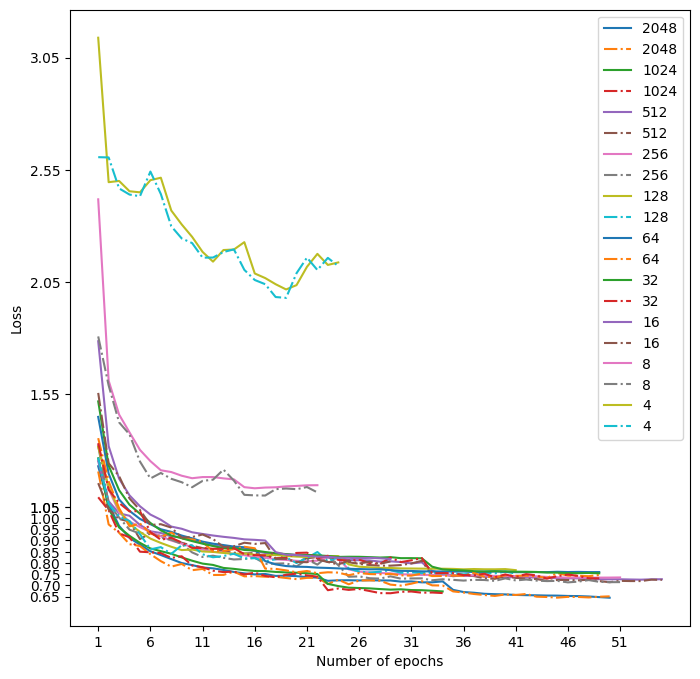
\includegraphics[width=400pt,height=350pt]{pictures/loss.png}
  \caption{Overview of the validation loss of the models trained with different dimensions. The y-axis represents the loss. The x-axis represents the number of epochs. The solid lines represent the mean training loss after each epoch. The dash dot line represents the mean validation loss after each epoch. The numbers in the legend represent the dimension of the latent space representations of the models. }
  \label{fig:loss}
\end{figure} 
 
\subsubsection{Evaluation of the Number of Semantic Subgroups}
\label{sec:conclu_pointnet_semantic}
Once the number of dimensions of the latent space representations is set to 512, next the optimum number of semantic subgroups is evaluated. Since the dataset consists of a large variety of objects, it is not possible to determine a fixed number of categories the objects are to be partitioned into. Thus, the evaluation of the number of subcategories is essential so that the ultimate goal of achieving a set of representative members of the dataset which generalizes the entire dataset quite well is achieved. 

\begin{table}[H]
  \setlength\extrarowheight{10pt}
  \caption{Results of the ConClu approach with PointNet autoencoder on 1000 datapoints when the dimension of the latent space representations is 512 and the number of semantic subgroups is 32. }
  \centering
  \begin{tabular}{|p{30pt}|p{50pt}|p{60pt}|p{50pt}|p{50pt}|p{50pt}|p{40pt}|}
    \toprule
    \ac{t-SNE} dim	& \ac{t-SNE} time & Clustering Algorithm & No. of Clusters & Clustering Time (seconds) & \ac{DBCV} score & \ac{DBCV} Time (seconds)\\
    \midrule
    \multirow{4}{30pt}{2}	& 3.555 & \ac{HDBSCAN}	& 279	& 0.620 & 0.185	& 689.203 \\ \cline{2-7} 
    & 3.731 & k-medoids	& 175	& 0.176 & -0.029	& 101.171 \\ \cline{2-7} 
    & 3.349 & Spectral	& 175	& 7.221 & 0.042 	& 100.748 \\ \cline{2-7}
    & 3.663 & Agglomerative	& 175	& 0.031 & -0.007	& 102.203 \\ 
    \bottomrule
  \end{tabular}
  \label{tab:conclu_k_32}
\end{table}

\begin{table}[H]
  \setlength\extrarowheight{10pt}
  \caption{Results of the ConClu approach on 1000 datapoints for multi-level \ac{HDBSCAN} clustering algorithm when the dimension of the latent space representations is 512 and the number of semantic subgroups is 32. }
  \centering
  \begin{tabular}{|l|l|l|l|l|l|}
    \toprule
    Level & Algorithm	& No. of Clusters	& No. of Outliers	& DBCV score	& \ac{DBCV} time (seconds)	\\  
    \midrule
    Level 1 & \ac{HDBSCAN} & 279	& 96	& 0.185	& 689.203 \\ \cline{1-6}
    Level 2 & \ac{HDBSCAN}	& 122	& 51	& 0.043	& 203.029 \\ 
    \bottomrule
  \end{tabular}
  \label{tab:conclu_k_32_levels}
\end{table}

\begin{table}[H]
  \setlength\extrarowheight{10pt}
  \caption{Results of the ConClu approach with PointNet autoencoder on 1000 datapoints when the dimension of the latent space representations is 512 and the number of semantic subgroups is 16. }
  \centering
  \begin{tabular}{|p{30pt}|p{50pt}|p{60pt}|p{50pt}|p{50pt}|p{50pt}|p{40pt}|}
    \toprule
    \ac{t-SNE} dim	& \ac{t-SNE} time & Clustering Algorithm & No. of Clusters & Clustering Time (seconds) & \ac{DBCV} score & \ac{DBCV} Time (seconds)\\
    \midrule
    \multirow{4}{30pt}{2}	& 3.797 & \ac{HDBSCAN}	& 291	& 0.140 & 0.182	& 244.248 \\ \cline{2-7} 
    & 3.557 & k-medoids	& 175	& 0.257 & -0.50	& 100.699 \\ \cline{2-7} 
    & 3.480 & Spectral	& 175	& 6.331 & 0.030	& 103.005 \\ \cline{2-7}
    & 3.731 & Agglomerative	& 175	& 0.033 & -0.007	& 104.203 \\ 
    \bottomrule
  \end{tabular}
  \label{tab:conclu_k_16}
\end{table}
Tab. \ref{tab:conclu_512} on Pg. 58 already shows the performance of the model when the dimensions of the latent space representation is 512 and the number of semantic subgroups is 64. Tab. \ref{tab:conclu_k_32} records the performance of the model when the number of semantic subgroups is set to 32. Tab. \ref{tab:conclu_k_32_levels} shows the performance of the multi-level \ac{HDBSCAN} algorithm on this model. The rest of the parameters for the experiments remains constant throughout this subsection. It is seen that the performance of the model with $k=32$ is comparable to the model with $k=64$. The \ac{DBCV} score for the model with $k=32$ is 0.185 while that of the model with $k=64$ is 0.186. In other words, even with fewer semantic subgroups the model could achieve comparable results. Moreover, the model for $k=32$ requires a training time of 28 hours for 39 epochs. Whereas, the model for $k=64$ requires a training time of 64 hours for 54 epochs. Thus, reducing the value of k by a factor of 2 also led t the decrease in the training time by a factor of 2.29. This also re-ensures the ultimate goal of the task. Fewer subcategories in the objects means the model will learn more "general" features of the objects and not the extremely intricate and instance-specific object features. This would help in objects of the dataset which actually capture the overall variance in the dataset. Tab. \ref{tab:conclu_k_16} and Tab. \ref{tab:conclu_k_8} shows the performance of the model when the dimension of the latent space representation is 512 and the number of semantic subgroups is 16 and 8 respectively.  Tab. \ref{tab:conclu_k_16_levels} records the performance of multi-level \ac{HDBSCAN} algorithm when the number of semantic subgroups is set to 16. The dimension of the latent space representations of all these models are 512. a batch size of 128 is used to train the models as mentioned earlier. The model for $k=16$ requires a training time of 37 hours for 63 epochs until convergence. Whereas, the model for $k=8$ requires a training time of 31 hours for 40 epochs. It is seen that the model with $k=16$ gives almost comparable results to that of the model with $k=32$. But it is observed that the model with $k=16$ takes longer training time for convergence as compared to the model with $k=32$. It is further noted that the performance of the model with $k=8$ degrades by a factor of 4.3\% as compared to that of the model with $k=8$.

\begin{table}[H]
  \setlength\extrarowheight{10pt}
  \caption{Results of the ConClu approach on 1000 datapoints for multi-level \ac{HDBSCAN} clustering algorithm when the dimension of the latent space representations is 512 and the number of semantic subgroups is 16. }
  \centering
  \begin{tabular}{|l|l|l|l|l|l|}
    \toprule
    Level & Algorithm	& No. of Clusters	& No. of Outliers	& DBCV score	& \ac{DBCV} time (seconds)	\\  
    \midrule
    Level 1 & \ac{HDBSCAN} & 291	& 110	& 0.182	& 244.248 \\ \cline{1-6}
    Level 2 & \ac{HDBSCAN}	& 117	& 38	& 0.033	& 57.618
    \\ 
    \bottomrule
  \end{tabular}
  \label{tab:conclu_k_16_levels}
\end{table}

\begin{table}[H]
  \setlength\extrarowheight{10pt}
  \caption{Results of the ConClu approach with PointNet autoencoder on 1000 datapoints when the dimension of the latent space representations is 512 and the number of semantic subgroups is 8. }
  \centering
  \begin{tabular}{|p{30pt}|p{50pt}|p{60pt}|p{50pt}|p{50pt}|p{50pt}|p{40pt}|}
    \toprule
    \ac{t-SNE} dim	& \ac{t-SNE} time & Clustering Algorithm & No. of Clusters & Clustering Time (seconds) & \ac{DBCV} score & \ac{DBCV} Time (seconds)\\
    \midrule
    \multirow{4}{30pt}{2}	& 3.018 & \ac{HDBSCAN}	& 291	& 0.140 & 0.139 	& 235.023 \\ \cline{2-7} 
    & 3.091 & k-medoids	& 175	& 0.191 & -0.092	& 98.415 \\ \cline{2-7} 
    & 3.101 & Spectral	& 175	& 6.810 & -0.027	& 96.898 \\ \cline{2-7}
    & 3.177 & Agglomerative	& 175	& 0.038 & -0.030	& 97.490 \\ 
    \bottomrule
  \end{tabular}
  \label{tab:conclu_k_8}
\end{table}

\begin{table}[H]
  \setlength\extrarowheight{10pt}
  \caption{Results of the ConClu approach with PointNet autoencoder on 1000 datapoints when the dimension of the latent space representations is 512 and the number of semantic subgroups is 128. }
  \centering
  \begin{tabular}{|p{30pt}|p{50pt}|p{60pt}|p{50pt}|p{50pt}|p{50pt}|p{40pt}|}
    \toprule
    \ac{t-SNE} dim	& \ac{t-SNE} time & Clustering Algorithm & No. of Clusters & Clustering Time (seconds) & \ac{DBCV} score & \ac{DBCV} Time (seconds)\\
    \midrule
    \multirow{4}{30pt}{2}	& 3.259 & \ac{HDBSCAN}	& 301	& 0.115 & 0.186 	& 332.309 \\ \cline{2-7} 
    & 4.356 & k-medoids	& 175	& 0.172 & -0.049	& 205.339 \\ \cline{2-7} 
    & 3.344 & Spectral	& 175	& 11.716 & 0.024	& 166.501 \\ \cline{2-7}
    & 5.815 & Agglomerative	& 175	& 0.049 & -0.041	& 170.280 \\ 
    \bottomrule
  \end{tabular}
  \label{tab:conclu_k_128}
\end{table} 

\begin{table}[H]
  \setlength\extrarowheight{10pt}
  \caption{Results of the ConClu approach with PointNet autoencoder on 1000 datapoints when the dimension of the latent space representations is 512 and the number of semantic subgroups is 4. }
  \centering
  \begin{tabular}{|p{30pt}|p{50pt}|p{60pt}|p{50pt}|p{50pt}|p{50pt}|p{40pt}|}
    \toprule
    \ac{t-SNE} dim	& \ac{t-SNE} time & Clustering Algorithm & No. of Clusters & Clustering Time (seconds) & \ac{DBCV} score & \ac{DBCV} Time (seconds)\\
    \midrule
    \multirow{4}{30pt}{2}	& 3.295 & \ac{HDBSCAN}	& 296	& 0.122 & 0.103	& 269.228 \\ \cline{2-7} 
    & 3.577 & k-medoids	& 175	& 0.308 & -0.045	& 139.550 \\ \cline{2-7} 
    & 3.751 & Spectral	& 175	& 11.623 & -0.004	& 167.611 \\ \cline{2-7}
    & 5.013 & Agglomerative	& 175	& 0.032 & -0.005	& 169.509 \\ 
    \bottomrule
  \end{tabular}
  \label{tab:conclu_k_4}
\end{table} 

\begin{table}[H]
  \setlength\extrarowheight{10pt}
  \caption{Results of the ConClu approach with PointNet autoencoder on 1000 datapoints when the dimension of the latent space representations is 512 and the number of semantic subgroups is 2. }
  \centering
  \begin{tabular}{|p{30pt}|p{50pt}|p{60pt}|p{50pt}|p{50pt}|p{50pt}|p{40pt}|}
    \toprule
    \ac{t-SNE} dim	& \ac{t-SNE} time & Clustering Algorithm & No. of Clusters & Clustering Time (seconds) & \ac{DBCV} score & \ac{DBCV} Time (seconds)\\
    \midrule
    \multirow{4}{30pt}{2}	& 4.469 & \ac{HDBSCAN}	& 289	& 0.126 & 0.085	& 320.217 \\ \cline{2-7} 
    & 3.364 & k-medoids	& 175	& 5.662 & -0.118 	& 155.136 \\ \cline{2-7} 
    & 3.349 & Spectral	& 175	& 5.662 & -0.089	& 115.978 \\ \cline{2-7}
    & 3.029 & Agglomerative	& 175	& 0.038 & -0.100	& 98.683 \\ 
    \bottomrule
  \end{tabular}
  \label{tab:conclu_k_2}
\end{table}

Tab. \ref{tab:conclu_k_128} shows the performance of the model when the dimension of the latent space representation is 512 and the number of semantic subgroups is 128. The model requires a training time of 58 hours for 36 epochs until convergence is reached.

\begin{figure}[H]
  \centering
  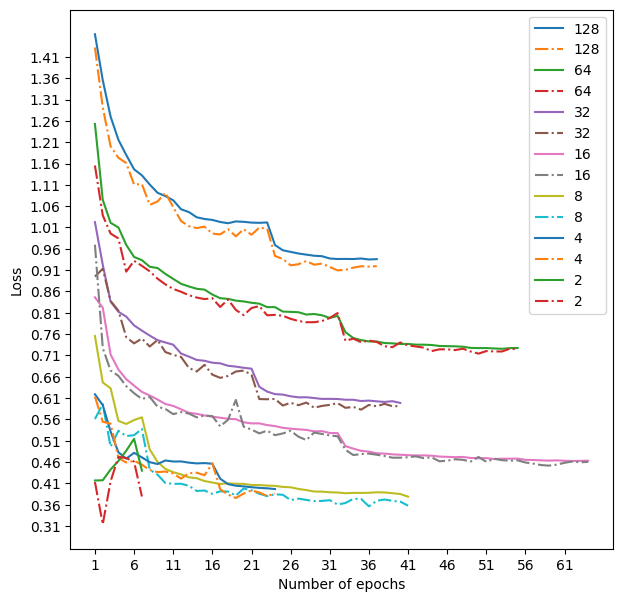
\includegraphics[width=400pt,height=300pt]{pictures/loss_k.png}
  \caption{Overview of the validation loss of the models trained with different values of semantic subgroups when dimension of the latent space representation is fixed to 512. The y-axis represents the loss. The x-axis represents the number of epochs. The solid lines represent the mean training loss after each epoch. The dash dot line represents the mean validation loss after each epoch. The numbers in the legend represent number of semantic subgroups in the objects.}
  \label{fig:loss_k}
\end{figure} 

It can be seen that the performance for the model with $k=128$ is comparable to the model with $k=32$. Also, the training time for the model with $k=32$ is much less compared to that of the model with $k=128$. Tab. \ref{tab:conclu_k_4} and Tab. \ref{tab:conclu_k_2} shows the performance of the model when the dimension of the latent space representation is 512 and the number of semantic subgroups is 4 and 2 respectively. The training time for the model with $k=4$ is 17 hours for 23 epochs. Similarly, the training time for the model with $k=2$ is 5 hours for 6 epochs. It can be observed that the performance of the models decline significantly when the number of semantic subgroups is too low. Thus, it can be concluded that the performance of the models increases with the increase in the number of semantic subgroups and then attains a saturation in the performance. In other words, the number of semantic subgroups doesn't effect the performance of the models as long as they are enough parts the objects are partitioned into. Tab. \ref{tab:conclu_k_128} shows the performance of the model when the dimension of the latent space representation is 512 and the number of semantic subgroups is 128. The model requires a training time of 58 hours for 36 epochs until convergence is reached. It can be seen that the performance for the model with $k=128$ is comparable to the model with $k=32$. Also, the training time for the model with $k=32$ is much less compared to that of the model with $k=128$. 


\subsubsection{Evaluation of the Batch Size for Training}
One of the most crucial hyperparameters to adjust in deep learning methods is batch size. Attempting to optimize convex functions involves an intrinsic trade-off between the advantages of larger and smaller batch sizes. One way to ensure convergence to the global optima of the objective function is to use a batch size equal to the entire dataset. But doing so comes at the expense of a slower empirical convergence to that optimal state. Also, it practically infeasible to load the entire dataset like the ABC dataset \cite{Koch_2019_CVPR} in this use-case all at once. However, it has been demonstrated empirically that employing lower batch sizes leads to a faster convergence to "good" solutions. Smaller batch sizes enable the model to "start learning before having to see all the data," which provides an easy explanation for this. A smaller batch size has the drawback of not guaranteeing that the model will eventually come to the global optima. It will oscillate between the global optima, remaining outside a certain $\epsilon$-ball of the optima, where $\epsilon$ is determined by the batch size to dataset ratio. Therefore, as mentioned in Ch. \ref{sec:hardware}, the largest batch size that could be fit in the GPU with the higher capacity is observed to be 256. Thus, to facilitate the training of multiple models for experimentation in the limited time frame parallelly, the performance of the models with batch sizes 64, 128 and 256 are evaluated. The dimension of the latent space representations of the all the models in this subsection is set to 512 and $k=32$ as discussed above. The learning rate is 0.001 and the decay factor for the learning rate is 0.1 as mentioned earlier. Tab. \ref{tab:conclu_k_32} on Pg. 63 already shows the performance of the model when batch size is 128. Tab. \ref{tab:conclu_batch_256} shows the performance of the model when the batch size is 256. The training time for this model is 40 hours for 43 epochs. Tab. \ref{tab:conclu_batch_256_levels} records the performance of the multi-level \ac{HDBSCAN} algorithm.
\begin{table}[H]
  \setlength\extrarowheight{10pt}
  \caption{Results of the ConClu approach with PointNet autoencoder on 1000 datapoints when the dimension of the latent space representations is 512, the number of semantic subgroups is 32 and the batch size for training the model is 256. }
  \centering
  \begin{tabular}{|p{30pt}|p{50pt}|p{60pt}|p{50pt}|p{50pt}|p{50pt}|p{40pt}|}
    \toprule
    \ac{t-SNE} dim	& \ac{t-SNE} time & Clustering Algorithm & No. of Clusters & Clustering Time (seconds) & \ac{DBCV} score & \ac{DBCV} Time (seconds)\\
    \midrule
    \multirow{4}{30pt}{2}	& 5.855 & \ac{HDBSCAN}	& 291	& 0.178 & 0.154 & 382.814 \\ \cline{2-7} 
    & 6.034 & k-medoids	& 175	& 0.384 & -0.040	& 146.189 \\ \cline{2-7} 
    & 5.365 & Spectral	& 175	& 13.660 & 0.026	& 145.207 \\ \cline{2-7}
    & 5.513 & Agglomerative	& 175	& 0.040 & -0.011	& 167.093 \\ 
    \bottomrule
  \end{tabular}
  \label{tab:conclu_batch_256}
\end{table}

\begin{table}[H]
  \setlength\extrarowheight{10pt}
  \caption{Results of the ConClu approach on 1000 datapoints for multi-level \ac{HDBSCAN} clustering algorithm when the dimension of the latent space representations is 512, the number of semantic subgroups is 32 and the batch size for training the model is 256. }
  \centering
  \begin{tabular}{|l|l|l|l|l|l|}
    \toprule
    Level & Algorithm	& No. of Clusters	& No. of Outliers	& DBCV score	& \ac{DBCV} time (seconds)	\\  
    \midrule
    Level 1 & \ac{HDBSCAN} & 291	& 92	& 0.154	& 382.814 \\ \cline{1-6}
    Level 2 & \ac{HDBSCAN} & 126	& 53	& 0.038	& 101.948 \\ 
    \bottomrule
  \end{tabular}
  \label{tab:conclu_batch_256_levels}
\end{table}

It is seen that this algorithm gives the second-best clustering results after \ac{HDBSCAN} algorithm. And the result is slightly better than that of spectral clustering. Quite naturally, the model takes longer to converge for a larger batch size. But performance of the model does not seem to improve as expected as compared to the model with batch size 128. The \ac{DBCV} of the \ac{HDBSCAN} algorithm is 0.185 for the earlier model, whereas for the model with batch size it appears to suffer a downfall in performance by 3.1\%.

\begin{table}[H]
  \setlength\extrarowheight{10pt}
  \caption{Results of the ConClu approach with PointNet autoencoder on 1000 datapoints when the dimension of the latent space representations is 512, the number of semantic subgroups is 32 and the batch size for training the model is 64. }
  \centering
  \begin{tabular}{|p{30pt}|p{50pt}|p{60pt}|p{50pt}|p{50pt}|p{50pt}|p{40pt}|}
    \toprule
    \ac{t-SNE} dim	& \ac{t-SNE} time & Clustering Algorithm & No. of Clusters & Clustering Time (seconds) & \ac{DBCV} score & \ac{DBCV} Time (seconds)\\
    \midrule
    \multirow{4}{30pt}{2}	& 5.454 & \ac{HDBSCAN}	& 300	& 1.080 & 0.177	& 730.026 \\ \cline{2-7} 
    & 6.732 & k-medoids	& 175	& 7.606 & -0.056	& 602.923 \\ \cline{2-7} 
    & 6.326 & Spectral	& 175	& 51.657 & 0.008	& 492.017 \\ \cline{2-7}
    & 6.129 & Agglomerative	& 175	& 0.489 & -0.007 &	481.838 \\ 
    \bottomrule
  \end{tabular}
  \label{tab:conclu_batch_64}
\end{table}

\begin{table}[H]
  \setlength\extrarowheight{10pt}
  \caption{Results of the ConClu approach on 1000 datapoints for multi-level \ac{HDBSCAN} clustering algorithm when the batch size for training the model is 64. }
  \centering
  \begin{tabular}{|l|l|l|l|l|l|}
    \toprule
    Level & Algorithm	& No. of Clusters	& No. of Outliers	& DBCV score	& \ac{DBCV} time (seconds)	\\  
    \midrule
    Level 1 & \ac{HDBSCAN} & 300	& 85	& 0.177	& 730.026 \\ \cline{1-6}
    Level 2 & \ac{HDBSCAN} & 128	& 41	& 0.035	& 210.596 \\ 
    \bottomrule
  \end{tabular}
  \label{tab:conclu_batch_64_levels}
\end{table}

\begin{figure}[H]
  \centering
  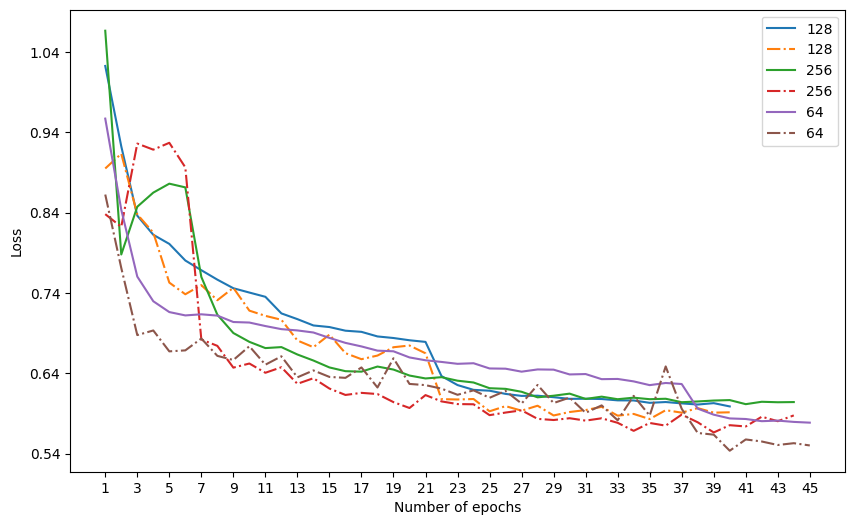
\includegraphics[width=400pt,height=200pt]{pictures/loss_batch.png}
  \caption{Overview of the validation loss of the models trained with different batch sizes when dimension of the latent space representation is fixed to 512 and the number of semantic subgroups to 32. The y-axis represents the loss. The x-axis represents the number of epochs. The solid lines represent the mean training loss after each epoch. The dash dot line represents the mean validation loss after each epoch. The numbers in the legend represent the batch size used for training the models. }
  \label{fig:loss_batch}
\end{figure} 

On the other hand, Tab. \ref{tab:conclu_batch_64} shows the performance of the model when the batch size is 64. Tab. \ref{tab:conclu_batch_64_levels} documents the performance of the multi-level \ac{HDBSCAN} algorithm on this model. The training time for this model is 36 hours for 44 epochs. The performance of the models is seen to improve from batch size 64 to 128 as expected. Fig. \ref{fig:loss_batch} gives an overview of the training and validation loss of the models with changing batch size. It can be observed that the validation loss of the models are quite comparable on convergence which can justify the reason behind no significant improvement of the models with different batch sizes. 

\subsubsection{Evaluation of the Effect of Early Stopping}
Determining an appropriate finite number of training epochs is a major challenge while developing machine learning models. If a model has too less epochs, then it would result to an underfit model whereas if the number of epochs is too large, then the model tends to memorize the training dataset and doesn't generalize well for unseen data \cite{Goodfellow-et-al-2016}. Therefore, the method of termination of the training when the model no longer improves its performance on the validation dataset is known as the early stopping mechanism. The patience parameter plays a very vital role in this mechanism. The model does not immediately terminate the training as soon as there is an increase in the validation loss. Rather it waits for a number of consecutive epochs defined by the patience parameter. And if the validation loss no longer decreases as compared to the least recorded validation loss, the training is then terminated.

\begin{table}[H]
  \setlength\extrarowheight{10pt}
  \caption{Results of the ConClu approach with PointNet autoencoder on 1000 datapoints when the patience for early stopping is 3, dimension of the latent space representations is 512, the number of semantic subgroups is 32 and the batch size for training the model is 128. }
  \centering
  \begin{tabular}{|p{30pt}|p{50pt}|p{60pt}|p{50pt}|p{50pt}|p{50pt}|p{40pt}|}
    \toprule
    \ac{t-SNE} dim	& \ac{t-SNE} time & Clustering Algorithm & No. of Clusters & Clustering Time (seconds) & \ac{DBCV} score & \ac{DBCV} Time (seconds)\\
    \midrule
    \multirow{4}{30pt}{2}	& 3.643 & \ac{HDBSCAN}	& 289	& 0.112 & 0.132	& 260.046 \\ \cline{2-7} 
    & 3.614 & k-medoids	& 175	& 0.101	& -0.054	& 115.333 \\ \cline{2-7} 
    & 3.535 & Spectral	& 175	& 5.567	& -0.008	& 114.561 \\ \cline{2-7}
    & 3.765 & Agglomerative	& 175	& 0.299	& -0.033	& 106.243 \\ 
    \bottomrule
  \end{tabular}
  \label{tab:conclu_patience_3}
\end{table}

\begin{table}[H]
  \setlength\extrarowheight{10pt}
  \caption{Results of the ConClu approach on 1000 datapoints for multi-level \ac{HDBSCAN} clustering algorithm when the patience for early stopping is 3. }
  \centering
  \begin{tabular}{|l|l|l|l|l|l|}
    \toprule
    Level & Algorithm	& No. of Clusters	& No. of Outliers	& DBCV score	& \ac{DBCV} time (seconds)	\\  
    \midrule
    Level 1 & \ac{HDBSCAN} & 289	& 98	& 0.132	& 260.046 \\ \cline{1-6}
    Level 2 & \ac{HDBSCAN} & 119	& 41	& -0.003	& 63.805 \\ 
    \bottomrule
  \end{tabular}
  \label{tab:conclu_patience_3_levels}
\end{table}
A patience of 3, 5, 7 and 10 have been evaluated in this subsection. The learning rate of 0.001 and a decay factor of 0.1 as mentioned earlier is used throughout the experiments recorded below. Tab. \ref{tab:conclu_patience_3} shows the performance of the model with patience 3. Tab. \ref{tab:conclu_patience_3_levels} records the performance of multi-level \ac{HDBSCAN} algorithm on this model. The model takes a training time of 10 hours for 10 epochs until convergence. Tab. \ref{tab:conclu_k_32} on Pg. 63 already shows the performance of the model when the patience parameter is set to 5. It requires a training time of 28 hours for 39 epochs. As expected the model with less patience has lower training time compared to that with a high patience. But it is that the performance of the model with less patience is worse as compared to that with higher patience. There is a 5\% decline in the quality of the performance. 

\begin{table}[H]
  \setlength\extrarowheight{10pt}
  \caption{Results of the ConClu approach with PointNet autoencoder on 1000 datapoints when the patience for early stopping is 7, dimension of the latent space representations is 512, the number of semantic subgroups is 32 and the batch size for training the model is 128. }
  \centering
  \begin{tabular}{|p{30pt}|p{50pt}|p{60pt}|p{50pt}|p{50pt}|p{50pt}|p{40pt}|}
    \toprule
    \ac{t-SNE} dim	& \ac{t-SNE} time & Clustering Algorithm & No. of Clusters & Clustering Time (seconds) & \ac{DBCV} score & \ac{DBCV} Time (seconds)\\
    \midrule
    \multirow{4}{30pt}{2}	& 3.731	& \ac{HDBSCAN}	& 298	& 0.126	& 0.199	& 293.794
    \\ \cline{2-7} 
    & 3.257	& k-medoids	& 175	& 0.134	& -0.037	& 116 \\ \cline{2-7} 
    & 3.340	& Spectral	& 175	& 9.391	& 0.011	& 94.393 \\ \cline{2-7}
    & 2.788	& Agglomerative	& 175	& 0.032	& -0.018	& 93.149 \\ 
    \bottomrule
  \end{tabular}
  \label{tab:conclu_patience_7}
\end{table}

\begin{table}[H]
  \setlength\extrarowheight{10pt}
  \caption{Results of the ConClu approach on 1000 datapoints for multi-level \ac{HDBSCAN} clustering algorithm when the patience for early stopping is 7. }
  \centering
  \begin{tabular}{|l|l|l|l|l|l|}
    \toprule
    Level & Algorithm	& No. of Clusters	& No. of Outliers	& DBCV score	& \ac{DBCV} time (seconds)	\\  
    \midrule
    Level 1 & \ac{HDBSCAN} & 298	& 99	& 0.199	& 293.794 \\ \cline{1-6}
    Level 2 & \ac{HDBSCAN} & 117	& 40	& 0.013	& 64.412
    \\ 
    \bottomrule
  \end{tabular}
  \label{tab:conclu_patience_7_levels}
\end{table}

\begin{table}[H]
  \setlength\extrarowheight{10pt}
  \caption{Results of the ConClu approach with PointNet autoencoder on 1000 datapoints when the patience for early stopping is 10, dimension of the latent space representations is 512, the number of semantic subgroups is 32 and the batch size for training the model is 128. }
  \centering
  \begin{tabular}{|p{30pt}|p{50pt}|p{60pt}|p{50pt}|p{50pt}|p{50pt}|p{40pt}|}
    \toprule
    \ac{t-SNE} dim	& \ac{t-SNE} time & Clustering Algorithm & No. of Clusters & Clustering Time (seconds) & \ac{DBCV} score & \ac{DBCV} Time (seconds)\\
    \midrule
    \multirow{4}{30pt}{2}	& 3.338	& \ac{HDBSCAN}	& 308	& 0.126	& 0.190	& 330.257 \\ \cline{2-7} 
    & 3.191	& k-medoids	& 175	& 0.288	& -0.051	& 166.315 \\ \cline{2-7} 
    & 3.072	& Spectral	& 175	& 7.785	& 0.013	& 156.930 \\ \cline{2-7}
    & 3.441	& Agglomerative	& 175	& 0.032	& -0.041	& 159.887 \\ 
    \bottomrule
  \end{tabular}
  \label{tab:conclu_patience_10}
\end{table}

Tab. \ref{tab:conclu_patience_7} and Tab. \ref{tab:conclu_patience_10} shows the performance of the models with patience 7 and 10 respectively. The former model takes a training time of 46 hours for 49 epochs. As expected, the model takes more number of epochs until convergence as compared to the model with patience 5. Also, the results for this model outperform the performance shown by the model with patience 3 and 5 as expected. Tab. \ref{tab:conclu_patience_7_levels} shows the performance of multi-level \ac{HDBSCAN} algorithm on this model. The \ac{DBCV} score attained by the \ac{HDBSCAN} algorithm is 0.199 by this model as coma
pared to the next best model with patience 5 which has the \ac{DBCV} score of 0.185. The model with patience 10 requires a training time of 30 hours for 42 epochs. But the performance of the model is seen to drop a bit as compared to the model with patience 7. Fig. \ref{fig:loss_early_stopping_patience} gives an overview of the training and validation loss of the models for different values of the patience parameter. As expected, the model with patience 10 has the least validation loss on convergence. Thus, weighing the training time of the models and their performance for the clustering task, the model with patience 7 is observed to have the best results. 

\begin{figure}[H]
  \centering
  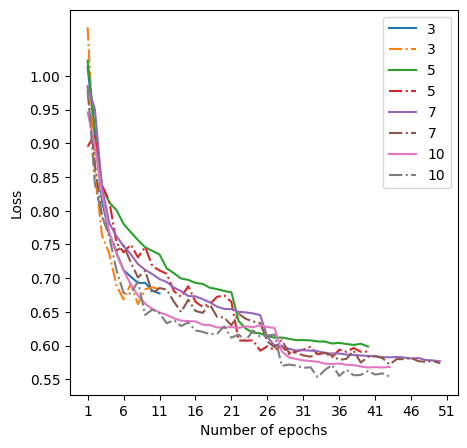
\includegraphics[width=350pt,height=250pt]{pictures/loss_early_stopping_patience.png}
  \caption{Overview of the validation loss of the models trained with different values of the patience parameter in early stopping when dimension of the latent space representation is fixed to 512, the number of semantic subgroups is 32 and batch size is 128. The y-axis represents the loss. The x-axis represents the number of epochs. The solid lines represent the mean training loss after each epoch. The dash dot line represents the mean validation loss after each epoch. The numbers in the legend represent the value of the patience parameter. }
  \label{fig:loss_early_stopping_patience}
\end{figure} 

\subsubsection{Evaluation of the Effect of Learning Rate}
The learning rate is one of the crucial hyperparameters when building a machine learning model. When the model weights are updated, it regulates how much the model is to be altered after calculating the estimated error. Carefully selecting the learning rate is extremely necessary because if the learning rate is too small, then the training process will be extremely low and it can get stuck at a local minima. Whereas, if the learning rate s too high, then the model can oscillate around the global optima without reaching a convergence. Tab. \ref{tab:conclu_32} on Pg. 60 already shows the performance of the model when the learning rate is set to 0.001. Tab. \ref{tab:conclu_lr_01} documents the performance of the model when the learning rate is set to 0.01. The model requires a training time of 28 hours for 40 epochs. It takes almost the same number of epochs to converge as does the model with learning rate 0.001. Furthermore, it can be observed that the performance of the model deteriorates when the learning rate is changed to 0.01 from 0.001. There is a 6\% degradation in performance when the learning rate is increased by a factor of 10. Tab. \ref{tab:conclu_lr_01_levels} shows the performance of the multi-level \ac{HDBSCAN} algorithm on this model.
\begin{table}[H]
  \setlength\extrarowheight{10pt}
  \caption{Results of the ConClu approach with PointNet autoencoder on 1000 datapoints when the learning rate is 0.01. }
  \centering
  \begin{tabular}{|p{30pt}|p{50pt}|p{60pt}|p{50pt}|p{50pt}|p{50pt}|p{40pt}|}
    \toprule
    \ac{t-SNE} dim	& \ac{t-SNE} time & Clustering Algorithm & No. of Clusters & Clustering Time (seconds) & \ac{DBCV} score & \ac{DBCV} Time (seconds)\\
    \midrule
    \multirow{4}{30pt}{2}	& 3.417	& \ac{HDBSCAN}	& 285	& 0.109	& 0.128	& 315.829 \\ \cline{2-7} 
    & 3.455	& k-medoids	& 175	& 0.246	& -0.038	& 147.585 \\ \cline{2-7} 
    & 3.270	& Spectral	& 175	& 6.347	& -0.057	& 156.651 \\ \cline{2-7}
    & 3.844	& Agglomerative	& 175	& 0.037	& -0.083	& 162.778 \\ 
    \bottomrule
  \end{tabular}
  \label{tab:conclu_lr_01}
\end{table} 

\begin{table}[H]
  \setlength\extrarowheight{10pt}
  \caption{Results of the ConClu approach on 1000 datapoints for multi-level \ac{HDBSCAN} clustering algorithm when the learning rate is 0.01. }
  \centering
  \begin{tabular}{|l|l|l|l|l|l|}
    \toprule
    Level & Algorithm	& No. of Clusters	& No. of Outliers	& DBCV score	& \ac{DBCV} time (seconds)	\\  
    \midrule
    Level 1 & \ac{HDBSCAN} & 285	& 107	& 0.128	& 315.829 \\ \cline{1-6}
    Level 2 & \ac{HDBSCAN} & 121	& 42	& -0.049	& 62.360 \\ 
    \bottomrule
  \end{tabular}
  \label{tab:conclu_lr_01_levels}
\end{table}

\subsubsection{Evaluation of the Effect of Decay Factor of the Learning Rate}

Keeping the learning rate and the rest of the parameters constant, experiments are performed to evaluate the effect of the decay factor of the learning rate on the performance of the model. The decay factor determines the value of the new learning rate as shown in Eq. \ref{eq:lr_decay} when the metrices for the performance of the model stops improving.

\begin{equation}
  \label{eq:lr_decay}
  new \; learning \; rate = decay \; factor \times current \; learning \; rate
\end{equation}

Tab. \ref{tab:conclu_32} on Pg. 60 already shows the performance of the model when the learning rate is set to 0.001 and the decay factor is 0.1. Tab. \ref{tab:conclu_lr_decay_5} shows the performance of the model when the learning rate remains constant at 0.001 but the decay factor is change to 0.5. Tab. \ref{tab:conclu_lr_decay_5_levels} shows the performance of multi-level \Ac{HDBSCAN} algorithm on this model. The performance of this model is seen to improve as compared to model with decay factor 0.1. There is almost a 3\% increase in the performance of the model. The decay factor is further increased and Tab. \ref{tab:conclu_lr_decay_9} records the performance of the model when the decay factor is 0.9. All the remaining parameters of the model remains constant. The model takes a training time of 20 hours for 26 epochs until convergence. A decrease in performance of the model is observed as compared to the model with decay rate 0.5.

\begin{table}[H]
  \setlength\extrarowheight{10pt}
  \caption{Results of the ConClu approach with PointNet autoencoder on 1000 datapoints when the learning rate is 0.001 and the decay factor is 0.5. }
  \centering
  \begin{tabular}{|p{30pt}|p{50pt}|p{60pt}|p{50pt}|p{50pt}|p{50pt}|p{40pt}|}
    \toprule
    \ac{t-SNE} dim	& \ac{t-SNE} time & Clustering Algorithm & No. of Clusters & Clustering Time (seconds) & \ac{DBCV} score & \ac{DBCV} Time (seconds)\\
    \midrule
    \multirow{4}{30pt}{2}	& 3.351	& \ac{HDBSCAN}	& 303	& 0.113	& 0.212	& 334.613 \\ \cline{2-7} 
    & 3.734	& k-medoids	& 175	& 0.273	& -0.033	& 164.001 \\ \cline{2-7} 
    & 3.192	& Spectral	& 175	& 6.865	& 0.003	& 109.385 \\ \cline{2-7}
    & 3.722	& Agglomerative	& 175	& 0.043	& -0.001	& 92.632 \\ 
    \bottomrule
  \end{tabular}
  \label{tab:conclu_lr_decay_5}
\end{table}

\begin{table}[H]
  \setlength\extrarowheight{10pt}
  \caption{Results of the ConClu approach on 1000 datapoints for multi-level \ac{HDBSCAN} clustering algorithm when the learning rate is 0.001 and the decay factor is 0.5. }
  \centering
  \begin{tabular}{|l|l|l|l|l|l|}
    \toprule
    Level & Algorithm	& No. of Clusters	& No. of Outliers	& DBCV score	& \ac{DBCV} time (seconds)	\\  
    \midrule
    Level 1 & \ac{HDBSCAN} & 303	& 71	& 0.212	& 334.613 \\ \cline{1-6}
    Level 2 & \ac{HDBSCAN} & 118	& 34	& 0.009	& 62.142 \\ 
    \bottomrule
  \end{tabular}
  \label{tab:conclu_lr_decay_5_levels}
\end{table}

\begin{table}[H]
  \setlength\extrarowheight{10pt}
  \caption{Results of the ConClu approach with PointNet autoencoder on 1000 datapoints when the learning rat is 0.001 and the decay factor is 0.9. }
  \centering
  \begin{tabular}{|p{30pt}|p{50pt}|p{60pt}|p{50pt}|p{50pt}|p{50pt}|p{40pt}|}
    \toprule
    \ac{t-SNE} dim	& \ac{t-SNE} time & Clustering Algorithm & No. of Clusters & Clustering Time (seconds) & \ac{DBCV} score & \ac{DBCV} Time (seconds)\\
    \midrule
    \multirow{4}{30pt}{2}	& 3.265	& \ac{HDBSCAN}	& 287	& 0.114	& 0.184	& 225.236 \\ \cline{2-7} 
    & 3.298	& k-medoids	& 175	& 0.144	& 0.010	& 95.764 \\ \cline{2-7} 
    & 4.107	& Spectral	& 175	& 14.298	& 0.036	& 116.901 \\ \cline{2-7}
    & 3.297	& Agglomerative	& 175	& 0.033	& 0.017	& 96.614 \\ 
    \bottomrule
  \end{tabular}
  \label{tab:conclu_lr_decay_9}
\end{table}

Fig. \ref{fig:loss_lr} gives an overview of the training and validation loss of the models for learning rate and decay factor of the learning rate used during training the models. Even with a lower higher learning rate, the model takes almost the same number of epoch until convergence. But it can be noticed that the model reaches a comparable validation loss quite early on as compared to the model with a lower learning rate. The model with learning rate  0.001 as decay factor 0.9 takes the least training time. 

\begin{table}[H]
  \setlength\extrarowheight{10pt}
  \caption{Results of the ConClu approach on 1000 datapoints for multi-level \ac{HDBSCAN} clustering algorithm when the learning rate is 0.001 and the decay factor is 0.9. }
  \centering
  \begin{tabular}{|l|l|l|l|l|l|}
    \toprule
    Level & Algorithm	& No. of Clusters	& No. of Outliers	& DBCV score	& \ac{DBCV} time (seconds)	\\  
    \midrule
    Level 1 & \ac{HDBSCAN} & 287	& 80	& 0.184	& 225.236 \\ \cline{1-6}
    Level 2 & \ac{HDBSCAN} & 120	& 46	& 0.044	& 56.283 \\ 
    \bottomrule
  \end{tabular}
  \label{tab:conclu_lr_decay_9_levels}
\end{table}

\begin{figure}[H]
  \centering
  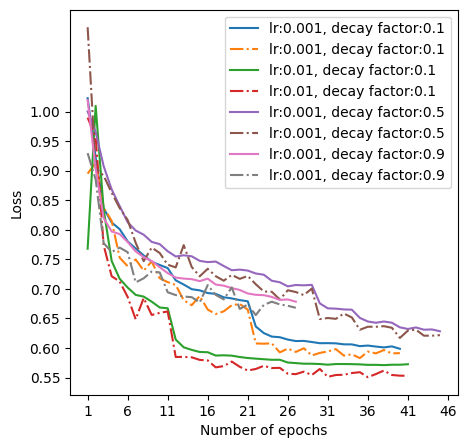
\includegraphics[width=300pt,height=280pt]{pictures/loss_lr.png}
  \caption{Overview of the validation loss of the models trained with different values of learning rate and decay factor of the learning rate when dimension of the latent space representation is fixed to 512, the number of semantic subgroups is 32 and batch size is 128. The y-axis represents the loss. The x-axis represents the number of epochs. The solid lines represent the mean training loss after each epoch. The dash dot line represents the mean validation loss after each epoch. The numbers in the legend represent the learning rate and decay factor of the learning rate.}
  \label{fig:loss_lr}
\end{figure} 

\subsection{ConClu Approach with Dynamic Graph Convolutional Neural Network as Backbone}
\label{sec:conclu_dgcnn}

As mentioned in Ch. \ref{sec:method}, two feature representation learning backbones are used for the experiments. Experiments with the \ac{DGCNN} as the backbone is recorded here. The performance of all the clustering algorithms are evaluated.

\subsubsection{Evaluation of dimension of feature space representations}
As discussed earlier, the dimension of the latent space representation is an extremely crucial parameter while training the network. Since the original dataset has the point clouds with 2048 points in each of them, for the sake of completeness of the experimentation, the evaluation are performed for all dimensions on a logarithmic scale of 2 from 1024 to down until 4. Tab. \ref{tab:dgcnn_1024} shows the experiments when the dimension of the latent space representations is set to be 1024. Tab. \ref{tab:dgcnn_1024_levels} shows the performance of multi-level \ac{HDBSCAN} model on this model. For all the models in this subsection, the number of nearest neighbors requires for a \ac{DGCNN} graph is set to 20 based on \cite{mei2022unsupervised}.

\begin{table}[H]
  \setlength\extrarowheight{10pt}
  \caption{Results of the ConClu approach with \ac{DGCNN} backbone on 1000 datapoints when the dimension of the latent space representation is 1024. }
  \centering
  \begin{tabular}{|p{30pt}|p{50pt}|p{60pt}|p{50pt}|p{50pt}|p{50pt}|p{40pt}|}
    \toprule
    \ac{t-SNE} dim	& \ac{t-SNE} time & Clustering Algorithm & No. of Clusters & Clustering Time (seconds) & \ac{DBCV} score & \ac{DBCV} Time (seconds)\\
    \midrule
    \multirow{4}{30pt}{2}	& 3.022	& \ac{HDBSCAN}	& 295	& 0.121 & 0.112	& 228.925 \\ \cline{2-7} 
    & 3.519 & k-medoids	& 175	& 0.151 & -0.067	& 92.043 \\ \cline{2-7} 
    & 3.212 & Spectral	& 175	& 6.712 & -0.038 	& 92.080 \\ \cline{2-7}
    & 3.683 & Agglomerative	& 175	& 0.037 & -0.089	& 124.850 \\ 
    \bottomrule
  \end{tabular}
  \label{tab:dgcnn_1024}
\end{table}

\begin{table}[H]
  \setlength\extrarowheight{10pt}
  \caption{Results of the ConClu approach on 1000 datapoints for multi-level \ac{HDBSCAN} clustering algorithm when the dimension of the latent space representation is 1024. }
  \centering
  \begin{tabular}{|l|l|l|l|l|l|}
    \toprule
    Level & Algorithm	& No. of Clusters	& No. of Outliers	& DBCV score	& \ac{DBCV} time (seconds)	\\  
    \midrule
    Level 1 & \ac{HDBSCAN} & 295	& 89	& 0.112	& 228.925  \\ \cline{1-6}
    Level 2 & \ac{HDBSCAN} & 132	& 40	& -0.035	& 86.639 \\ 
    \bottomrule
  \end{tabular}
  \label{tab:dgcnn_1024_levels}
\end{table}

\begin{table}[H]
  \setlength\extrarowheight{10pt}
  \caption{Results of the ConClu approach with \ac{DGCNN} backbone on 1000 datapoints when the dimension of the latent space representation is 512. }
  \centering
  \begin{tabular}{|p{30pt}|p{50pt}|p{60pt}|p{50pt}|p{50pt}|p{50pt}|p{40pt}|}
    \toprule
    \ac{t-SNE} dim	& \ac{t-SNE} time & Clustering Algorithm & No. of Clusters & Clustering Time (seconds) & \ac{DBCV} score & \ac{DBCV} Time (seconds)\\
    \midrule
    \multirow{4}{30pt}{2}	& 3.214 & \ac{HDBSCAN}	& 299	& 0.125 & 0.129	& 327.926 \\ \cline{2-7} 
    & 3.739 & k-medoids	& 175	& 0.248 & -0.060	& 162.210 \\ \cline{2-7} 
    & 3.212 & Spectral	& 175	& 6.712 & -0.038 & 92.080 \\ \cline{2-7}
    & 3.683 & Agglomerative	& 175	& 0.037 & -0.089	& 124.850 \\ 
    \bottomrule
  \end{tabular}
  \label{tab:dgcnn_512}
\end{table}

It is observed that training the models with the \ac{DGCNN} backbone takes extremely large training time. The model with the dimension of latent space representation of 1024 takes 168 hours for 37 epochs until convergence. This is more than twice the time requires for the model with PointNet autoencoder as backbone, which requires 73 hours for 65 epochs. This is because of the dynamic graph creation step involved for this method in each epoch before every convolutional layer. Also the performance of this model is a little worse as compared to the model with PointNet autoencoder as the backbone with same dimension for the latent space representation, the performance of which is recorded in Tab. \ref{tab:conclu_1000} on Pg. 53. Tab. \ref{tab:dgcnn_512} records the performance of the model when the dimension of the latent space representation is 512. 

\begin{table}[H]
  \setlength\extrarowheight{10pt}
  \caption{Results of the ConClu approach on 1000 datapoints for multi-level \ac{HDBSCAN} clustering algorithm when the dimension of the latent space representation is 512. }
  \centering
  \begin{tabular}{|l|l|l|l|l|l|}
    \toprule
    Level & Algorithm	& No. of Clusters	& No. of Outliers	& DBCV score	& \ac{DBCV} time (seconds)	\\  
    \midrule
    Level 1 & \ac{HDBSCAN} & 299	& 119	& 0.129	& 327.926  \\ \cline{1-6}
    Level 2 & \ac{HDBSCAN} & 126	& 45	& -0.071	& 64.300 \\ 
    \bottomrule
  \end{tabular}
  \label{tab:dgcnn_512_levels}
\end{table}  

\begin{table}[H]
  \setlength\extrarowheight{10pt}
  \caption{Results of the ConClu approach with \ac{DGCNN} backbone on 1000 datapoints when the dimension of the latent space representation is 256. }
  \centering
  \begin{tabular}{|p{30pt}|p{50pt}|p{60pt}|p{50pt}|p{50pt}|p{50pt}|p{40pt}|}
    \toprule
    \ac{t-SNE} dim	& \ac{t-SNE} time & Clustering Algorithm & No. of Clusters & Clustering Time (seconds) & \ac{DBCV} score & \ac{DBCV} Time (seconds)\\
    \midrule
    \multirow{4}{30pt}{2}	& 3.374	& \ac{HDBSCAN}	& 278	& 0.112	& 0.098	& 240.169 \\ \cline{2-7} 
    & 3.673	& k-medoids	& 175	& 0.171	& -0.151	& 103.629 \\ \cline{2-7} 
    & 3.579	& Spectral	& 175	& 6.933	& -0.078	& 105.700 \\ \cline{2-7}
    & 3.722	& Agglomerative	& 175	& 0.044	& -0.001	& 92.631 \\ 
    \bottomrule
  \end{tabular}
  \label{tab:dgcnn_256}
\end{table}

\begin{table}[H]
  \setlength\extrarowheight{10pt}
  \caption{Results of the ConClu approach with \ac{DGCNN} backbone on 1000 datapoints when the dimension of the latent space representation is 128. }
  \centering
  \begin{tabular}{|p{30pt}|p{50pt}|p{60pt}|p{50pt}|p{50pt}|p{50pt}|p{40pt}|}
    \toprule
    \ac{t-SNE} dim	& \ac{t-SNE} time & Clustering Algorithm & No. of Clusters & Clustering Time (seconds) & \ac{DBCV} score & \ac{DBCV} Time (seconds)\\
    \midrule
    \multirow{4}{30pt}{2}	& 3.498	& \ac{HDBSCAN}	& 289	& 0.118	& 0.103	& 250.010 \\ \cline{2-7} 
    & 3.839	& k-medoids	& 175	& 0.131	& -0.116	& 106.311 \\ \cline{2-7} 
    & 3.559	& Spectral	& 175	& 6.662	& -0.108	& 103.972 \\ \cline{2-7}
    & 3.590	& Agglomerative	& 175	& 0.045	& -0.099	& 104.450 \\ 
    \bottomrule
  \end{tabular}
  \label{tab:dgcnn_128}
\end{table}
Tab. \ref{tab:dgcnn_512_levels} documents the performance of multi-level \ac{HDBSCAN} algorithm on this model. All other parameters of the model remains constant. This model takes a training time of 231 hours for 60 epochs. This is four times the time requires by the model when PointNet autoencoder as the backbone. Even with such high training time, the performance of the model is seen to deteriorate by atleast $3\%$ in case of \ac{HDBSCAN} algorithm and atmost $5\%$ in case of agglomerative clustering algorithm. Table. \ref{tab:dgcnn_256} records the performance of the model when the dimension is further reduced to 256. On reducing the dimension by a factor of 2, the model training time requires by the model also decreased by a factor of 2. Now the model requires a training time of 120 hours for 31 epochs. But unlike the model with the PointNet autoencoder as backbone, this model had a degradation in the performance when the dimension is reduced to 256. There is a 3\% decrease in performance for the \ac{HDBSCAN} algorithm and roughly $5\%$ degradation for the k-medoids algorithm and spectral clustering algorithm. However, the performance of the agglomerative clustering algorithm remains almost similar. For the purpose of completeness of the evaluation, the dimension of the model is further reduced to 64, 32, 16, 8 and 4. Tab. \ref{tab:dgcnn_64} and Tab. \ref{tab:dgcnn_32} are the models with dimension 64 and 32 respectively. 

\begin{table}[H]
  \setlength\extrarowheight{10pt}
  \caption{Results of the ConClu approach with \ac{DGCNN} backbone on 1000 datapoints when the dimension of the latent space representation is 64. }
  \centering
  \begin{tabular}{|p{30pt}|p{50pt}|p{60pt}|p{50pt}|p{50pt}|p{50pt}|p{40pt}|}
    \toprule
    \ac{t-SNE} dim	& \ac{t-SNE} time & Clustering Algorithm & No. of Clusters & Clustering Time (seconds) & \ac{DBCV} score & \ac{DBCV} Time (seconds)\\
    \midrule
    \multirow{4}{30pt}{2}	& 3.430	& \ac{HDBSCAN}	& 289	& 0.113	& 0.083	& 253.259 \\ \cline{2-7} 
    & 3.572	& k-medoids	& 175	& 0.137	& -0.074	& 107.411 \\ \cline{2-7} 
    & 3.384	& Spectral	& 175	& 6.879	& -0.090	& 105.169 \\ \cline{2-7}
    & 3.298	& Agglomerative	& 175	& 0.030	& -0.104	& 104.248 \\ 
    \bottomrule
  \end{tabular}
  \label{tab:dgcnn_64}
\end{table}

\begin{table}[H]
  \setlength\extrarowheight{10pt}
  \caption{Results of the ConClu approach with \ac{DGCNN} backbone on 1000 datapoints when the dimension of the latent space representation is 32. }
  \centering
  \begin{tabular}{|p{30pt}|p{50pt}|p{60pt}|p{50pt}|p{50pt}|p{50pt}|p{40pt}|}
    \toprule
    \ac{t-SNE} dim	& \ac{t-SNE} time & Clustering Algorithm & No. of Clusters & Clustering Time (seconds) & \ac{DBCV} score & \ac{DBCV} Time (seconds)\\
    \midrule
    \multirow{4}{30pt}{2}	& 3.390	& \ac{HDBSCAN}	& 284	& 0.179	& 0.088	& 308.699 \\ \cline{2-7} 
    & 4.151	& k-medoids	& 175	& 0.304	& -0.098	& 178.198 \\ \cline{2-7} 
    & 4.199	& Spectral	& 175	& 34.680	& -0.065	& 185.643 \\ \cline{2-7}
    & 3.067	& Agglomerative	& 175	& 0.032	& -0.110	& 99.183 \\ 
    \bottomrule
  \end{tabular}
  \label{tab:dgcnn_32}
\end{table} 

As mentioned earlier, early stopping criteria is used during the training of the models to prevent overfitting. A patience of 5 is used for all the models in this subsection. Similar to the setup of the ConClu approach with PointNet autoencoder as backbone. A very high number of epochs is set for the training so that the training always terminates only when the early stopping criteria is triggered. Thus, the number of epochs is set to 200. The model with dimension 64 takes a training time of 90 hours for 33 epochs. The performance of the model is seen to deteriorate as compared to that of the models of higher dimension. Tab. \ref{tab:dgcnn_32} records the performance of the model when the dimension of the laten space representation is set to 32. 

\begin{table}[H]
  \setlength\extrarowheight{10pt}
  \caption{Results of the ConClu approach with \ac{DGCNN} backbone on 1000 datapoints when the dimension of the latent space representation is 4. }
  \centering
  \begin{tabular}{|p{30pt}|p{50pt}|p{60pt}|p{50pt}|p{50pt}|p{50pt}|p{40pt}|}
    \toprule
    \ac{t-SNE} dim	& \ac{t-SNE} time & Clustering Algorithm & No. of Clusters & Clustering Time (seconds) & \ac{DBCV} score & \ac{DBCV} Time (seconds)\\
    \midrule
    \multirow{4}{30pt}{2}	& 3.204	& \ac{HDBSCAN}	& 286	& 0.117	& -0.078	& 235.378 \\ \cline{2-7} 
    & 3.317 & k-medoids	& 175	& 0.144	& -0.135	& 100.929 \\ \cline{2-7} 
    & 3.133	& Spectral	& 175	& 3.587	& -0.059	& 102.188 \\ \cline{2-7}
    & 3.225	& Agglomerative	& 175	& 0.033	& -0.100	& 99.532 \\ 
    \bottomrule
  \end{tabular}
  \label{tab:dgcnn_4}
\end{table}

\begin{figure}[H]
  \centering
  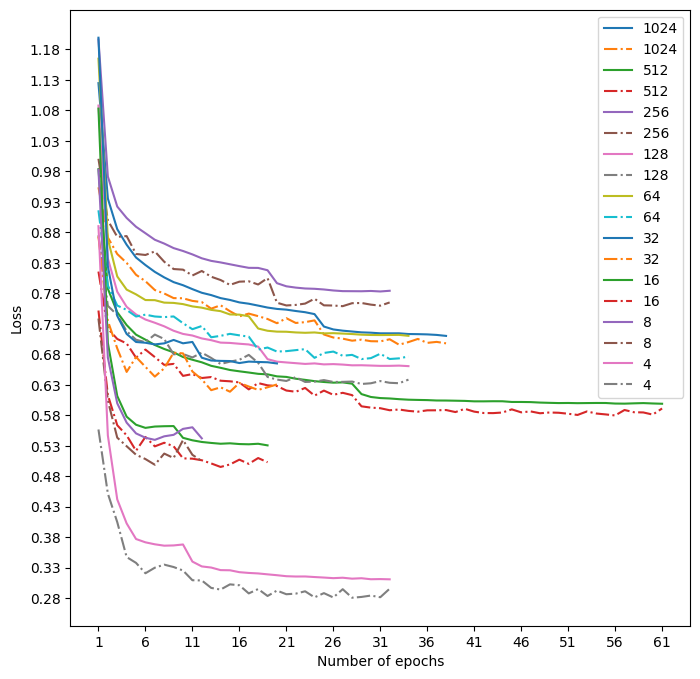
\includegraphics[width=300pt,height=300pt]{pictures/loss_dgcnn.png}
  \caption{Overview of the training and validation loss of the models trained with different values of dimension of the latent space representation when the number of nearest neighbors is fixed to 20. The y-axis represents the loss. The x-axis represents the number of epochs. The solid lines represent the mean training loss after each epoch. The dash dot line represents the mean validation loss after each epoch. The numbers in the legend represent the dimension of the latent space representations.}
  \label{fig:loss_dgcnn}
\end{figure} 

The model requires a training time of 70 hours for 19 epochs until convergence. The performance of the model is quite comparable to the model with dimension 64. Further reducing the dimension of the latent space representations degrades the performance of the models even more. Fig. \ref{fig:loss_dgcnn} gives an overview of all the models trained with \ac{DGCNN} as the backbone of the model for different sizes of the latent space representation. It can be observed that the validation loss is least when the model has dimensionality 4. But looking into the performance of the model while clustering the dataset, it can be seen that the performance is significantly worse. This could be a result of overfitting of the model. In the absence of enough dimensions of the latent space representations, the model is not properly calibrated. It learns the noise in the training dataset which makes it more confident in the predictions in the validation set which reduces the loss. But these "confident" predictions are actually incorrect predictions. Thus, there is a significant decrease in performance while clustering the dataset. Tab. \ref{tab:dgcnn_4} records the performance of the model when the dimensionality of the latent space representations is set to 4. 

\subsubsection{Evaluation of the effect of increasing datapoints} 
It is important to check that the results obtained on a small subset of the entire dataset can be relied upon for deriving conclusions on the entire dataset. Tab. \ref{tab:dgcnn_512} on Pg. 75 already shows the results of the model for 1000 datapoints.
\begin{table}[H]
  \setlength\extrarowheight{10pt}
  \caption{Results of the ConClu approach with \ac{DGCNN} backbone on 2000 datapoints when the dimension of the latent space representation is 512.}
  \centering
  \begin{tabular}{|p{30pt}|p{50pt}|p{60pt}|p{50pt}|p{50pt}|p{50pt}|p{40pt}|}
    \toprule
    \ac{t-SNE} dim	& \ac{t-SNE} time & Clustering Algorithm & No. of Clusters & Clustering Time (seconds) & \ac{DBCV} score & \ac{DBCV} Time (seconds)\\
    \midrule
    \multirow{4}{30pt}{2}	& 7.034	& \ac{HDBSCAN}	& 591	& 0.225	& 0.182	& 3.596.855 \\ \cline{2-7} 
    & 6.511	& k-medoids	& 175	& 0.213	& -0.202	& 409.159 \\ \cline{2-7} 
    & 6.730	& Spectral	& 175	& 26.729	& -0.129	& 410.735 \\ \cline{2-7}
    & 6.666	& Agglomerative	& 175	& 0.102	& -0.17	& 399.792 \\ 
    \bottomrule
  \end{tabular}
  \label{tab:dgcnn_2000}
\end{table}

Tab. \ref{tab:dgcnn_2000} records the performance of the model when the number of datapoints are increased to 2000. It can be seen that the time for dimensionality reduction with \ac{t-SNE} increases linearly on increasing the number of datapoints. But as mentioned earlier, the time for calculating the \ac{DBCV} score increases exponentially and not linearly. Similar to the observations with the PointNet autoencoder as backbone, the performance increases for the \ac{HDBSCAN} algorithm but not quite for the rest of the algorithms. This is because of the fact that more datapoints invariably mean more dense clusters when the number of clusters remain constant. Also, the \ac{DBCV} score  being a density based clustering validation index shows a better score for density based clustering algorithms. 

\begin{table}[H]
  \setlength\extrarowheight{10pt}
  \caption{Results of the ConClu approach on 2000 datapoints for multi-level \ac{HDBSCAN} clustering algorithm when the dimension of the latent space representation is 512. }
  \centering
  \begin{tabular}{|l|l|l|l|l|l|}
    \toprule
    Level & Algorithm	& No. of Clusters	& No. of Outliers	& DBCV score	& \ac{DBCV} time (seconds)	\\  
    \midrule
    Level 1 & \ac{HDBSCAN} & 591	& 193	& 0.129	& 327.926 \\ \cline{1-6}
    Level 2 & \ac{HDBSCAN} & 223	& 73	& -0.054	& 604.703
    \\ 
    \bottomrule
  \end{tabular}
  \label{tab:dgcnn_2000_levels}
\end{table} 

\begin{table}[H]
  \setlength\extrarowheight{10pt}
  \caption{Results of the ConClu approach with \ac{DGCNN} backbone on 5000 datapoints when the dimension of the latent space representation is 512. }
  \centering
  \begin{tabular}{|p{30pt}|p{50pt}|p{60pt}|p{50pt}|p{50pt}|p{40pt}|p{50pt}|}
    \toprule
    \ac{t-SNE} dim	& \ac{t-SNE} time & Clustering Algorithm & No. of Clusters & Clustering Time (seconds) & \ac{DBCV} score & \ac{DBCV} Time (seconds)\\
    \midrule
    \multirow{4}{30pt}{2}	& 17.516	& \ac{HDBSCAN}	& 1.486	& 0.647	& 0.185	& 120280.203 \\ \cline{2-7} 
    & 18.025	& k-medoids	& 175	& 0.550	& -0.409	& 2.696.609 \\ \cline{2-7} 
    & 6.730	& Spectral	& 175	& 26.729	& -0.129	& 410.735 \\ \cline{2-7}
    & 6.666	& Agglomerative	& 175	& 0.102	& -0.17	& 399.792 \\ 
    \bottomrule
  \end{tabular}
  \label{tab:dgcnn_5000}
\end{table}

\begin{table}[H]
  \setlength\extrarowheight{10pt}
  \caption{Results of the ConClu approach on 5000 datapoints for multi-level \ac{HDBSCAN} clustering algorithm when the dimension of the latent space representation is 512. }
  \centering
  \begin{tabular}{|l|l|l|l|l|l|}
    \toprule
    Level & Algorithm	& No. of Clusters	& No. of Outliers	& DBCV score	& \ac{DBCV} Time (seconds)	\\  
    \midrule
    Level 1 & \ac{HDBSCAN} & 1486	& 510	& 0.185	& 120280.203 \\ \cline{1-6}
    Level 2 & \ac{HDBSCAN} & 609	& 176	& -0.026	& 20.460.755 \\ \cline{1-6}
    Level 3 & \ac{HDBSCAN} & 265	& 106	& -0.205	& 4595.876 \\
    \bottomrule
  \end{tabular}
  \label{tab:dgcnn_5000_levels}
\end{table} 

Tab. \ref{tab:dgcnn_2000_levels} shows the performance of multi-level \ac{HDBSCAN} algorithm on this model. Tab. \ref{tab:dgcnn_5000} records the performance of the model when the number of datapoints are further increased to 5000. Tab. \ref{tab:dgcnn_5000_levels} shows the performance of multi-level \ac{HDBSCAN} algorithm on this model. As the number of datapoints increase, the number of iterations of the multi-level \ac{HDBSCAN} algorithm requires to reach a total number of clusters less than or equal to 175 also increases. Hence, it requires 3 levels for 5000 objects. It is to be noted that the performance of the multi-level \ac{HDBSCAN} algorithm improves with increase in the number of datapoints. 

\subsection{Comparison Between the PointNet Autoencoder Backbone and the Dynamic Graph Convolutional Neural Network backbone}

As observed earlier, the training time for the model with \ac{DGCNN} as the backbone is quite higher as compared to the models with PointNet autoencoder as backbone. And even with higher training time, the performance of the models are significantly worse. Amongst the models with \ac{DGCNN} as the backbone, the one with dimensionality 512 has the best results. But it requires a training time of 231 hours (i.e. almost 10 days) as compared to the model with PointNet autoencoder as backbone which requires 28 hours. Thus, fine-tuning the model for the rest of the hyperparameters with the \ac{DGCNN} backbone when the dimensionality is 512 is infeasible within the duration of this thesis as is possible for the model with PointNet autoencoder backbone, the results of which are recorded in Ch. \ref{sec:conclu_with_pointnet}. An overview of the training of the two models with different backbone but same dimensionality of the latent space representations is shown in Fig. \ref{fig:loss_camparison}. It can be observed that the ultimate validation loss for both the models are extremely comparable where the model with PointNet autoencoder backbone converges faster than the one with \ac{DGCNN} backbone. Thus, it seemed to be a rather practical choice to fine-tune the former model for the ultimate goal of this thesis. 

\begin{figure}[H]
  \centering
  \includegraphics[width=300pt,height=300pt]{pictures/loss_comparison.png}
  \caption{Overview of the training and validation loss of the models trained with different backbones - PointNet autoencoder and \ac{DGCNN} when the dimension of the latent space representation is set to 512. The y-axis represents the loss. The x-axis represents the number of epochs. The solid lines represent the mean training loss after each epoch. The dash dot line represents the mean validation loss after each epoch. The legend represent the backbone of the model. }
  \label{fig:loss_camparison}
\end{figure}

\subsubsection*{Calculating the Similarity of the Test Dataset with the Representative Objects}

Once the representative objects are obtained, it is necessary to compare how similar they are compared to the objects in the test dataset. Hausdorff distance is commonly used to calculate the similarity between two point clouds.

\begin{table}[H]
  \setlength\extrarowheight{10pt}
  \caption{Similarity metric for the ConClu approach with PointNet Autoencoder backbone.}
  \centering
  \begin{tabular}{|p{50pt}|p{50pt}|p{50pt}|p{60pt}|p{50pt}|}
    \toprule
    Dataset Size(Whole)	& No. of  representative objects	& Dataset Size(Test)	& Clustering Algorithm	& Average Hausdorff Distance\\
    \midrule
    949647	& 94	& 49981	& multi-level \ac{HDBSCAN} &  0.170 \\ \cline{1-5} 
    949647	& 175	& 49981	& k-medoids	& 0.134 \\ \cline{1-5}
    949647	& 175	& 49981	& Spectral	&	0.155  \\ \cline{1-5}
    949647	& 175	& 49981	& Agglomerative	& 0.138 \\   
    \bottomrule
  \end{tabular}
  \label{tab:pointnet_sim}
\end{table}

 Table- \ref{tab:pointnet_sim} shows the similarity metric of the ConClu approach with the PointNet Autoencoder as backbone. It can be seen that the k-medoids has the minimum Hausdorff distance which is quite comparable to agglomerative clustering followed by spectral clustering and eventually multi-level \ac{HDBSCAN} algorithm. This can be due to the fact that the traditional spectral clustering algorithm and agglomerative clustering doesn't give medoids of the cluster but cluster centres. But to ensure that the cluster centres are actual members of the dataset, Hausdorff distance is used to calculate the medoid of the clusters from the respective cluster members.  Because of this usage of Hausdorff distance in calculating the medoid, it is possible that when Hausdorff distance is used to calculate the ultimate similarity of the test dataset and the representative members, it slightly favoured the clustering algorithm which already used it for calculating the cluster medoid. Also to make it consistent with spectral clustering and agglomerative clustering, Hausdorff distance is also used as the pairwise distance metric during the k-medoids. Overall, it is to be noted further that even if the average distance for multi-level \ac{HDBSCAN} is a little more  than the rest of the algorithm, the variation isn't quite drastic. Tab. \ref{tab:dgcnn_sim} shows the similarity metric of the ConClu approach with the \ac{DGCNN} as backbone. It is observed that the results for both the backbones are very similar. Hence, it is not conclusive enough to use just this similarity metric to choose a suitable network for the purpose. 

\begin{table}[H]
  \setlength\extrarowheight{10pt}
  \caption{Similarity metric for the ConClu approach with \ac{DGCNN} backbone.}
  \centering
  \begin{tabular}{|p{50pt}|p{50pt}|p{50pt}|p{60pt}|p{40pt}|}
    \toprule
    Dataset Size(Whole)	& No. of  representative objects	& Dataset Size(Test)	& Clustering Algo	& Average Hausdorff Distance\\
    \midrule
    949647	& 94	& 49981	& multi-level \ac{HDBSCAN} &  0.170 \\ \cline{1-5} 
    949647	& 175	& 49981	& k-medoids	& 0.133 \\ \cline{1-5}
    949647	& 175	& 49981	& Spectral	&	0.152  \\ \cline{1-5}
    949647	& 175	& 49981	& Agglomerative	& 0.137 \\   
    \bottomrule
  \end{tabular}
  \label{tab:dgcnn_sim}
\end{table}

\subsection{Results}

Observing the results of the experimentations it is evident that the \ac{HDBSCAN} algorithm has significantly better performance as compared to any other clustering algorithm. But it had a major drawback of not having any control on the ultimate number of clusters obtained in the end. To circumnavigate this issue, the idea of multi-level \ac{HDBSCAN} is proposed. This naturally degrades the \ac{DBCV} score to some extent because the least-dense region within a cluster is no longer more dense as compared to the region in-between clusters but it has 2 important benefits. It had a control on the ultimate number of representative objects of the dataset which is very crucial in the present use-case. Also often times, it is observed that even though the result of this algorithm is not up to the mark as of \ac{HDBSCAN} algorithm, it is still better or at  least comparable to the next best algorithm, i.e. the spectral clustering algorithm. Furthermore, another significant benefit of multi-level \ac{HDBSCAN} algorithm as compared to spectral clustering is that the latter takes significantly higher time to cluster such a large dataset as compared to the former. Even in evaluations recorded in Ch. \ref{sec:experiments} it can be seen that the time taken by the spectral clustering algorithm is quite high as compared to any other algorithm. The multi-level \ac{HDBSCAN} algorithm takes 0.8 seconds to cluster 1000 datapoints, whereas spectral clustering takes 7.2 seconds for the same task. This phenomenon is even intensified when the number of samples increase from 1000 datapoints to 1 million datapoints. Spectral clustering takes roughly 20 days to form 175 clusters from the entire dataset, whereas the multi-level \ac{HDBSCAN} takes as less as 3 hours. This is because spectral clustering has a time complexity of $O(N^3)$ for a dataset with $N$ objects. Also, it is observed that the multi-level \ac{HDBSCAN} algorithm had better performance in most cases as compared to spectral clustering. Thus, it is inefficient to use such large clustering time for worse performance. The ultimate goal of this thesis is to identify "good" source data that represents the variance of the entire dataset.

\begin{figure}[t]
  \centering
  \includegraphics[width=400pt,height=300pt]{pictures/all_objs.PNG}
  \caption{Some of the representative members of the ABC dataset\cite{Koch_2019_CVPR} obtained on applying multi-level \ac{HDBSCAN} algorithm on the feature representations obtained from the ConClu approach with PointNet Autoencoder backbone.}
  \label{fig:all_hdbscan_objs}
\end{figure}

It is observed that the objects obtained after the applying the clustering algorithms are quite diverse in nature. Although there is no known objective way to determine what qualifies as a "good" source object in case of unsupervised learning, the diversity in the objects obtained in the end quite ensures the fulfillment of the task in hand. Fig. \ref{fig:all_hdbscan_objs} shows some of the cluster representatives obtained after applying the multi-level \ac{HDBSCAN} algorithm. Only some objects were chosen from the entire set of representative objects for the sake of visualization. It can be seen that the representative objects of the dataset are quite diverse in nature. Ranging from an ellipse shaped ring, an aircraft to a dumbbell, the objects are quite different from one another. Thus, weighing the pros and cons of the two different backbones and the 5 different clustering algorithm, it can be concluded that the ConClu approach with the PointNet Autoencoder gives the best model for the generation of the latent space representations of te objects in the dataset. Furthermore, weighing the performance of the clustering algorithm under different setup and the overall time required by the clustering algorithms, the multi-level \ac{HDBSCAN} algorithm seems to be a practical choice for this scenario. The \ac{HDBSCAN} algorithm has better performance compared to the multi-level \ac{HDBSCAN} algorithm because more number of clusters would naturally mean more smaller but denser clusters. But since it has no control on the number of clusters it returns and mostly returns a large number of clusters in the presence of a large dataset. Having such a high number of cluster representatives isn't feasible for further tasks in the current setup at \ac{IPA}. This is why the maximum number of cluster representatives is set to 175. Under this particular constraint, the multi-level \ac{HDBSCAN} algorithm is the best choice for clustering algorithm in this use-case. 
\cleardoublepage

\section{Summary}
\subsection{Conclusion}
The primary goal of this thesis was to create a source library to be used for transfer learning approaches in bin picking applications at \ac{IPA}. This is achieved at the end of the thesis work. A chosen number of objects collectively represent the entire ABC dataset \cite{Koch_2019_CVPR} consisting of one million 3D point clouds. It can be qualitatively justified that the representative members of the dataset are quite diverse in nature.

\vspace{5mm}

A deep learning algorithm is implemented and evaluated which is capable of processing any dataset containing points clouds of the objects. The algorithm is capable of generating latent space representations of the objects with any number of dimensions as deemed fit according to the user. The two backbones used in this network are the PointNet Autoencoder and the \ac{DGCNN}. This thesis also evaluates the performance of different clustering algorithms for the purpose of generating representative members of the dataset in hand which constitute as a diverse collection of source data. The clustering algorithms evaluated in this procedure are k-medoids, \ac{HDBSCAN}, spectral clustering and agglomerative clustering. A new concept called multi-level \ac{HDBSCAN} algorithm is also proposed in this thesis keeping the limitations in this use-case in mind which is illustrated in the next section.  Thus, this thesis is able to develop a framework of the network and the data which can be used further by the transfer learning approaches. 

\vspace{5mm}

The best performance is attained by the model with PointNet Autoencoder as backbone. Several hyperparameter tuning is performed to improve the performance of the model. Using this model has a plethora of benefits. The performance of the clustering algorithms on the output of this model is better as compared to both the existent network at \ac{IPA} and also the model with the \ac{DGCNN} backbone. The training time for this model is significantly lower which facilitated further hyperparameter-tuning resulting in improved results. 

\subsection{Limitations}
\label{sec:limitations}
There were several challenges encountered during the course of the thesis work. Each sample had 2048 points in the point cloud of the objects. This is essential for learning the features of the objects to eventually come up with accurate feature representation. But this also makes it a dataset with high dimensionality. To tackle such large dataset with individual sample having high dimensions, the concept of dimensionality reduction had to be incorporated. This resulted in additional time in the pipeline and also loss of information about the data to some extent. But this step is extremely necessary to achieve the final goal of the thesis. There is loss of information about the objects due to dimensionality reduction. But there is no way to quantize how much of the information is actually lost. The hardware available served as a challenge when dealing with large datasets like the ABC dataset \cite{Koch_2019_CVPR}. There are systems available at \ac{IPA} with \ac{GPU}s of higher capacity. But since there are multiple ongoing projects, they were not available for use during this thesis.

\vspace{5mm}

Another very obvious problem already existing in these type of tasks is evaluating the performance of the clustering algorithms in unsupervised learning paradigm. Though the availability of the \ac{DBCV} index helped this situation to some extent, it incorporated challenges of its own. Calculating the \ac{DBCV} score depended heavily on the number of features of the datapoints. In the presence of a large number of features, it is impossible to work with such high dimensional data in the available hardware setup mentioned in Ch. \ref{sec:hardware}. This is a primary reason why the concept of dimensionality reduction had to be used. Because of how the \ac{DBCV} algorithm works, evaluating the performance of the clustering algorithms while considering all the datapoints together is unfeasible. So the performance of the clustering algorithm had to be evaluated for a smaller subset of the dataset. This made it crucial to verify if the performance followed a similar trend even for higher number of datapoints and the results obtained while working with a smaller subset of the dataset is enough to derive logical conclusions.

\vspace{5mm}

Furthermore, a unifying evaluation metric that gives the same preference to globular and non-globular clusters is not available. The prevalent metrics tend to have a bias towards either of the two. In the presence of high dimensional dataset such as the ABC dataset \cite{Koch_2019_CVPR}, it is not possible to visualize the entire dataset in high dimensional space to decide whether the clusters are convex or non-convex in nature. Thus, the decision of which metric to use cannot be relied on the visualization of the representations of the actual objects. Therefore, it is completely based on the theoretical aspect and the expected outcomes of the same. 

\vspace{5mm}
As documented in Ch. \ref{sec:conclu_dgcnn}, it is seen that the training time of the ConClu approach with the \ac{DGCNN} backbone is significantly high in the current hardware setup as mentioned in \ref{sec:hardware}. In the absence of better hardware resources it is infeasible to conduct further studies in this limited time frame with this backbone in the search of better results. 

\subsection{Future Scope}

The source library and the framework suggested in this thesis can be used for further transfer learning tasks down the pipeline. The performance of those approaches with the existing library at \ac{IPA} can be compared to that of this newly created source library. Finding a better clustering evaluation metric while keeping the current limitations is an open point for further research. 

\vspace{5mm}

Furthermore, it is seen that the performance of spectral clustering algorithm is often comparable to that of multi-level \ac{HDBSCAN} algorithm. But it required an impractical amount of time for the spectral clustering algorithm to converge. The hyperparameters in spectral clustering could be fine-tuned to evaluate if it ameliorates the convergence time. Moreover, in the presence of better hardware resources like \ac{GPU} clusters it could be possible to perform spectral clustering algorithm on such large dataset in a practical duration of time. 

\vspace{5mm}

Also, it is noticed that the network with \ac{DGCNN} backbone is quite 
computationally expensive. Better hardware setup might facilitate fine-tuning of its hyperparameters to further improve the results. Having better hardware setup would also mean more number of samples could be evaluated at once during calculating the \ac{DBCV} score. This could further help in improving the quality of the results. The values of certain parameters are set according to \cite{mei2022unsupervised}, specially in the  Sinkhorn-Knopp algorithm module. Better domain knowledge could possibly improve the performance, if the hyperparameters are fine-tuned further. Therefore, if some of the limitations can be circumnavigated, the performance can be improved even further.


\section*{List of Acronyms}
\pagenumbering{roman}
\addcontentsline{toc}{section}{List of Acronyms}

\begin{acronym}
    \acro{AI}{Artificial Intelligence}
    \acro{CAD}{Computer-Aided Design}
    \acro{CNN}{Convolutional Neural Network}
    \acro{CPU}{Central Processing Unit}
    \acro{DBCV}{Density Based Clustering Validation}
    \acro{DBSCAN}{Density-Based Spatial Clustering of Applications with Noise}
    \acro{DGCNN}{Dynamic Graph Convolutional Neural Network}
    \acro{DSC}{Density Sparseness of a Cluster}
    \acro{DSPC}{Density Separation of a Pair of Clusters}
    \acro{EM}{Expectation Maximization}
    \acro{FCN}{Fully Connected Network}
    \acro{GAN}{Generative Adversarial Network}
    \acro{GB}{Giga Bytes}
    \acro{GPU}{Graphics Processing Unit}
    \acro{HDBSCAN}{Hierarchical Density-Based Spatial Clustering of Applications with Noise}
    \acro{IPA}{Fraunhofer Institute for Manufacturing Engineering and Automation} 
    \acro{KD}{K-Dimensional}
    \acro{KL}{Kullback–Leibler divergence}
    \acro{k-NN}{k-Nearest Neighbor}
    \acro{LDA}{Linear Discriminant Analysis}
    \acro{LiDAR}{Light Detection and Ranging}
    \acro{LIN}{linear}
    \acro{ML}{Machine Learning}
    \acro{MLP}{Multi Layer Perceptron}
    \acro{MRD}{Mutual Reachability Distance}
    \acro{MST}{Minimum Spanning Trees}
    \acro{NDA}{Normal Discriminant Analysis}
    \acro{DFA}{Discriminant Function Analysis}
    \acro{PTP}{point-to-point}
    \acro{PCA}{Principal Component Analysis}
    \acro{ReLU}{Rectified Linear Unit}
    \acro{RAM}{Random Access Memory}
    \acro{RGB}{Red Green Blue}
    \acro{RL}{Reinforcement Learning}
    \acro{RNN}{Recurrent Neural Network}
    \acro{stop-grad}{stop-gradient}
    \acro{SVM}{Support Vector Machines}
    \acro{TCP}{Tool Center Point} 
    \acro{t-SNE}{t-distributed Stochastic Neighbor Embedding}
    \acro{VAE}{Variational Autoencoders}
       
    
\end{acronym}
\addcontentsline{toc}{section}{List of Figures}
\listoffigures
\addcontentsline{toc}{section}{List of Tables}
\listoftables
\cleardoublepage
\addcontentsline{toc}{section}{List of Symbols}
\section*{List of Symbols}
\begin{table}[H]
    \setlength\extrarowheight{5pt}
    \centering
    \begin{tabular}{|p{70pt}|p{30pt}|p{270pt}|}
      \toprule
      Symbol	& Unit	& Description\\
      \midrule
      $\mathit{a_{pts}coredist}$ & - & The inverse of the density of each object with respect to all other objects inside its cluster  \\
      $\mathit{B_k}$ & - & In-between cluster dispersion matrix \\
      $\mathit{Cov}$ & - & Covariance \\
      $\mathit{C_S}$ & - & Set of critical points \\
      $\mathit{d_H(X,Y)}$ & - & Hausdorff distance between two points $X$ and $Y$ \\
      $\mathit{d_{mreach}}$ & - & Mutual reachability distance \\
      $\mathit{D_w}$ & - & Euclidean distance between two datapoints \\
      $\mathit{\mathcal{D_S}}$ & - & Source domain \\
      $\mathit{\mathcal{D_T}}$ & - & Target domain \\
      $\mathit{e'_{ijm}}$ & - & EdgeConv operator \\
      $F$ & - & Point Wise feature matrix of point cloud P \\
      $\mathit{f}$ & - & Symmetric function \\
      $f_{p_i}$ & - & Point wise feature vector \\
      $f_{\varphi}$ & - & Encoder backbone with parameters $\varphi$ \\
      $\mathit{g}$ & - & Gaussian distribution kernel \\
      $G_{PO}$	& -	& Pose of an object with respect to the gripper \\
      $H$ &- & Average cross entropy loss \\
      $\mathit{G(V,E)}$ & - & Graph G with vertices V and edges E \\
      $\mathit{hausdorff(P_1, P_2)}$ & - & Hausdorff distance between two point clouds $P_1$ and $P_2$ \\
      $h_{\theta}$ & - & Non-linear function \\
      $KNN$ & - & Distance to the $k$-th nearest neighbor \\
      $\lambda$ & - & Regularization parameter \\
      $\mathcal{L}_{con}$	& -	& Contrastive loss \\
      $\mathit{L_{global}}$ & - & GLobal symmetric loss \\
      $\mathit{L_{orth}}$ & - & Orthogonal Loss \\
      $\mathit{L_{reg}}$ & - & Loss for regularization \\      
      $\mathcal{L}_{tri}$	& -	& Triplet loss \\
      $\mathit{M_{ij}}$ & - & $M_{ij}$ is the distance between the centroids of the clusters $i$ and $j$ \\
      $\mathit{N}$ & - & Number of datapoints \\
      $P$ & - & Point cloud \\
        
      \bottomrule
    \end{tabular}
\end{table}
\begin{flushright}
  Continued to next page
\end{flushright}

\begin{table}[H]
  \setlength\extrarowheight{5pt}
  \centering
  \begin{tabular}{|p{70pt}|p{30pt}|p{270pt}|}
    \toprule
    Symbol	& Unit	& Description\\
    \midrule    
    $P^a, \; P^b$ & -& Two augmented views of point cloud P \\
    $p_i$ & - & Each point in a point cloud \\
    $\mathit{p_{ij}}$ & - & Joint conditional probability \\
    $p_{j|i}$ & - & Probability that the point $x_i$ has $x_j$ as its neighbor \\
    $\mathit{P(\mathcal{X})}$ & - & Marginal probability distribution of $\mathcal{X}$ \\
    $\mathit{q}$ & - & Projection head \\
    $\mathit{q_{ij}}$ & - & Joint probability distribution \\
    $\mathit{R}$ & - & Measure for cluster similarity in David-Bouldin Index \\
    $\mathbb{R}^\mathit{K}$ & - & K-dimensional real number \\
    $\square$ & - & Symmetric aggregation function \\
    $\mathbf{S}$ & - & Class probability matrix \\
    $\mathit{S_c}$ & - & Silhouette Coefficient \\
    $\mathit{S_{CH}}$ & - & Calinski-Harabasz Index \\
    $\mathit{S_i}$ & - & Dispersion measure of cluster $i$ \\
    $\mathit{\mathcal{T_S}}$ & - & Source task \\
    $\mathit{\mathcal{T_T}}$ & - & Target task \\
    $\mathit{var}$ & - & Variance \\
    $\mathit{V_C}$ & - & Validity index of cluster C \\
    $\mathit{W_k}$ & - & Within-between cluster dispersion matrix \\
    $W_{PG}$	& -	& Goal pose of the end-effector with respect to the world coordinate system \\
    $W_{PO}$	& -	& Pose of an object with respect to some world coordinate
    system \\
    $\mathcal{X}$ & - & Feature space \\
    $\mathit{\mathcal{Y}}$& - & Label space \\     
    \bottomrule
  \end{tabular}
\end{table}

% \printunsrtglossary[type=symbols,style=long,title={List of Symbols}]


% =========================================================================
\printbibliography[heading=bibintoc,title={Bibliography}]
\end{document}
